\documentclass[subfig,blackref,approvalform]{drexel-thesis} % library copy
%\documentclass[subfig,blackref,draftspace]{drexel-thesis} % for committee
%\documentclass[draft,subfig,blackref,draftwatermark]{drexel-thesis} % draft copy

\usepackage{verbatim}
\usepackage{amsmath}
\usepackage{amsthm}
\usepackage{array}
\usepackage{setspace}
\usepackage{dsfont} % Fancy R^n symbol
\usepackage{placeins}   % To allow pictures to flush after a section

% fncychap clobbers \appendix with a silly implementation that breaks
% hyperlinks to appendix chapters.  Work around this by ignoring their
% implementation completely.
\let\temporaryAppendix\appendix
%\usepackage[Conny]{fncychap}  % Nicer style used for distribution
\usepackage[]{fncychap}
\let\appendix\temporaryAppendix

\usepackage{tikz}
\usepackage{tkz-berge}
\usetikzlibrary{shapes}

% Spacings between the chapter top and to the text
\newcommand{\chaptertopspacing}{10}
\newcommand{\chaptertotextspacing}{-10}
\newcommand{\chaptertopspacingSTAR}{10}
\newcommand{\chaptertotextspacingSTAR}{-10}

\iffinal{}{  % Library format requires numbered footnotes
\renewcommand{\thefootnote}{$\dagger$}	% Daggers for footnote markers style
}

% Convenience functions
\newcommand{\B}[1]{ {\bf #1} }      		% Bold text for matrices
\newcommand{\Z}{\mathcal{Z}}				% Partition function
\newcommand{\HAM}{\mathcal{H}}		% Hamiltonian
\newcommand{\qp}[0]{(\B{q},\B{p})}  % Cannonical variables (q,p) 
\newcommand{\pfrac}[2]{\frac{\partial #1}{\partial #2}} 	% partial 1 /partial 2 
\newcommand{\ket}[1]  {\left | \, #1 \right \rangle}			% bra-ket notation
\newcommand{\abs}[1]{\left\vert #1 \right\vert}		% vert bars for averages
\newcommand{\norm}[1]{\left\Vert #1 \right\Vert}	% taller vert bars for the norm
\newcommand{\evalat}[1]{\left. #1 \right \vert}	% ex. evaluating the int. at its limits
\newcommand{\set}[1]{\left\{ #1 \right\}}					% squigle brackets for sets
\newcommand{\avg}[1]{\left< #1 \right>}					% angle brackets for averages
\newcommand{\paren}[1]{\left( #1 \right)}					% grows parentheses to the correct size
\newcommand{\brackets}[1]{\left[ #1 \right]}			% grows square brackets
\newcommand{\braces}[1]{\left \{ #1 \right \}}
\newcommand{\piecewisebrace}[1]{\left \{ #1 \right .} % Useful for piecewise functions

\newcommand{\ie}{i.e.\ }
\newcommand{\eg}{e.g.\ }
\newcommand{\cf}{c.f.\ }
\newcommand{\chem}[1]{\ensuremath{\mathrm{#1}}} % Chemical formula

\DeclareMathOperator*{\minor}{minor\,}
\DeclareMathOperator*{\sgn}{\mathbf{sgn}\,}
\DeclareMathOperator*{\rootof}{RootOf\,}


\newcommand{\figurewidthSINGLE}{0.8\textwidth}
\newcommand{\figurewidthDOUBLE}{0.45\textwidth}
\newcommand{\figurewidthTRIPLE}{0.35\textwidth}

\newcommand{\CHI}[2]{\chi_{#1 #2}} % Cluster Counting function


% Partition block notation
\newcommand*\pblock[3]{
	\tikz[baseline=(char.base)]{
		\node[ellipse,draw,inner sep=2pt] (char) {$#1$};
	} ^{#2}_{#3}
}

\newcommand{\Go}{\text{G}\bar{\text{o}}}
\newcommand{\GO}{\textbf{G}}
\newcommand{\CHIX}{\mathbf{X}}
\newcommand{\KP}{k_+}
\newcommand{\KM}{k_-}
\newcommand{\KPMAX}{k_+^*}

% -----------------------------------------------------------------------------
% Add the CC logo to the copyright page and spruce it up a bit
\renewcommand\copyrighttextCCBYSA{
\\[2 em]
\begin{quote}
\begin{center}
\includegraphics[width=.3\textwidth]{pictures/cc_logo.pdf} \\[2 em]
\end{center} 
This work is licensed under the terms of the Creative Commons Attribution NonCommercial ShareAlike Version $3.0$. The license is available at \url{http://creativecommons.org/licenses/by-nc-sa/3.0/}.
\end{quote}
}

% -----------------------------------------------------------------------------
% Enviorment for temporarily removing the page footer
\newcommand{\suppressfooter}
{%
\fancyfoot[RE,LO,LE,RO]{}
\renewcommand{\footrulewidth}{0.0pt}
}%

\newcommand{\restorefooter}
{%
\fancyfoot[RE,LO]{\scshape\leftmark}
\fancyfoot[LE,RO]{\scshape\rightmark}
\renewcommand{\footrulewidth}{.4pt}
}%

% -----------------------------------------------------------------------------
% Simple command for inline figures (does not count towards a normal figure)

\newcommand{\inlinespacing}{1em}
\newcommand{\inlineframebox}[2]{
\vspace{1em}
\newline
\fbox{
\begin{minipage}[]{.95 \linewidth}
\begin{center}
#1 \\
#2
\end{center}
\end{minipage}
}
\vspace{1em}
\newline
}

\newcommand{\inlinembox}[2]{
\vspace{1em}
\newline
\begin{minipage}[]{.95 \linewidth}
\begin{center}
#1 \\
#2
\end{center}
\end{minipage}
\vspace{1em}
\newline
}


% -----------------------------------------------------------------------------
% Custom styling for quote boxes, use \epigraph

\definecolor{quotationcolour}{HTML}{F0F0F0}
\definecolor{quotationmarkcolour}{HTML}{1F3F81}

\newcommand{\epiline}{\hrule \vskip -.2em \hrule}
% Massively humongous opening quotation mark.
\newcommand{\hugequote}[1]{%
  \fontsize{42}{48}\selectfont \color{quotationmarkcolour} \textbf{#1}
  \vskip -.5em
}

\newcommand{\epigraph}[2]{%
  \smallskip
 \begin{center}
%  \hspace{1em}
  \colorbox{quotationcolour}{%
    \parbox{.8\textwidth}{%
    \epiline \vskip 1em 
    #1
    \begin{flushright}\textsc{#2}\end{flushright}
    \epiline
    }
  }
  \end{center}
  \medskip
}

\newcommand{\epigraphshort}[1]{%
  \smallskip
 \begin{center}
%  \hspace{1em}
  \colorbox{quotationcolour}{%
    \parbox{.8\textwidth}{%
    \epiline \vskip 1em 
     \begin{center}
    #1
    \end{center}

    \epiline
    }
  }
  \end{center}
  \medskip
}

% -----------------------------------------------------------------------------
% custom DRAFT MARK

\usepackage[]{datetime} 
\usepackage[allpages]{draftmark}

\iffinal{}{
\draftmarksetup{
  angle=0,scale=.34,
  color=red!45!blue!25,xcoord=117,ycoord=-129,
  mark={  \raggedright \mmddyyyydate (DRAFT)\\ \today} }
}

% -----------------------------------------------------------------------------
% Customize fncychap settings
\iffinal{}{
	\ChRuleWidth{1.5pt}
	\ChTitleLowerCase
	\ChTitleVar{\Huge \sc}
	}

% -----------------------------------------------------------------------------
% tighten the fncychap spacings, TeX code taken from
% http://tex.stackexchange.com/questions/13357/fncychap-package-reduce-vertical-gap-space-between-header-and-chapter-heading

\makeatletter
\renewcommand*{\@makechapterhead}[1]{%
  \iffinal{\setstretch{\@ssp}}{}
  
  \vspace*{\chaptertopspacing\p@}%
  {\parindent \z@ \raggedright \normalfont
    \ifnum \c@secnumdepth >\m@ne
      \if@mainmatter%%%%% Fix for frontmatter, mainmatter, and backmatter 040920
        \DOCH
      \fi
    \fi
    \interlinepenalty\@M
    \if@mainmatter%%%%% Fix for frontmatter, mainmatter, and backmatter 060424
      \DOTI{#1}%
    \else%
      \DOTIS{#1}%
    \fi
    \vspace*{\chaptertotextspacing\p@}
  }
  \iffinal{\setstretch{\@dsp}}{}  
}


 \renewcommand*{\@makeschapterhead}[1]{%
  \vspace*{\chaptertopspacingSTAR\p@}%
  {\parindent \z@ \raggedright
    \normalfont
    \interlinepenalty\@M
    \DOTIS{#1}
    \vskip \chaptertotextspacingSTAR\p@
  }}
 
\makeatother


% -----------------------------------------------------------------------------
% redefine abstract from drexel-thesis since the spacing is now wrong
\makeatletter
\renewenvironment{abstract}{%
  \listed@schapter{\abstractname}%
  \blanklines{-0}%
    \begin{center}
      \setstretch{\@ssp}%
      \@DUT@title\\
      \@DUT@author\\
      \ifdaring{%
        \ifnum\c@@DUT@advisors=\@ne%
        Advisor:
        \else%
        Advisors:
        \fi}{}
      \@DUT@advisor\\
    \end{center}
  \blanklines{4}%
  \setstretch{\@dsp}%
  \@nobreaktrue
  \@afterindentfalse
  \@afterheading
}{%
  \par\setstretch{\@ssp}%
}
\makeatother


\includeonly{
     tex/preamble,              %Dedications, acknowledgments, TOC, and abstract
     tex/preface,               %Biophysics topical comments
     tex/introduction,          %CHAPTER: Introduction
     tex/methods,               %CHAPTER: Computational Methods   
     Neutrino_ Oscillation/Neutrino_Oscillation, %CHAPTER: Entropic paper
     DC_Results/Double_Chooz,     %CHAPTER: WL paper
     AA/Articulated_Arm,           %CHAPTER: Conformational States Under Crowding
     Paraphotons/Paraphotons,       %CHAPTER: Clustering and Kinetics
     }

%\setkeys{Gin}{draft} % Draft mode on the pictures

\usepackage[square,numbers,sort&compress,comma]{natbib} % fancy citation extensions
\bibliographystyle{unsrtnat}

\author{Edward Angus Damon}
\title{Measurement of Paraphotons in the Double Chooz Experiment Using Articulated Arm Calibration Methods}
\DUTmonth{May}
\DUTyear{2014}
\degree{Doctor of Philosophy}
\advisor{Dr. Jelena Maricic}
\copyrighttext{\copyrighttextCCBYSA}

\tikzstyle{vertex}=[circle,fill=black!25,minimum size=10pt,inner sep=2pt]
\tikzstyle{Nvertex}=[circle,fill=white!25,minimum size=10pt,inner sep=2pt]
\tikzstyle{LabelStyle}=[fill=white,sloped]

\tikzstyle{big_vertex}=[circle,fill=red!15,minimum size=50pt,inner sep=2pt,draw=black!50]
\tikzstyle{med_vertex}=[circle,fill=red!10,minimum size=35pt,inner sep=2pt,draw=black!50]

\tikzstyle{macrostate_vertex}=[inner sep=3pt,draw=black!70]


\newcommand{\vertexshiftamount}{2.5}
\newcommand{\tikzpicscale}{1.5}

\newcommand{\TIKZenergylevel}{

  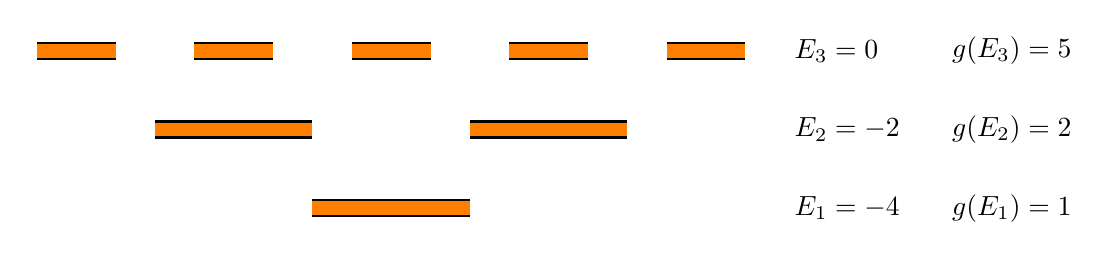
\begin{tikzpicture}
    \tikzset{level/.style   = {thick,
        double          = orange,
        double distance = 5pt}}
    
    \def\Espace{9};
    \def\Gspace{11};
    
    % Draw the energy levels.
    \draw[level] (3,0)  -- (5,0) node[right]{};
    \draw[] (\Espace,0) node[right] {$E_1=-4$};
    \draw[] (\Gspace,0) node[right] {$g(E_1)=1$};
    
    \draw[level] (1,1) -- (3,1) node[right] {};
    \draw[level] (5,1) -- (7,1) node[right] {};
    \draw[] (\Espace,1) node[right] {$E_2=-2$};
    \draw[] (\Gspace,1) node[right] {$g(E_2)=2$};
    
    \def\v{.5}; 
    \draw[level] (-1+\v,2) -- (0+\v,2) node[right] {};
    \draw[level] (1+\v,2) -- (2+\v,2) node[right] {};
    \draw[level] (3+\v,2) -- (4+\v,2) node[right] {};
    \draw[level] (5+\v,2) -- (6+\v,2) node[right] {};
    \draw[level] (7+\v,2) -- (8+\v,2) node[right] {};
    \draw[] (\Espace,2) node[right] {$E_3=0$};
    \draw[] (\Gspace,2) node[right] {$g(E_3)=5$};
  \end{tikzpicture}
}

\newcommand{\TIKZenergylevelSHORT}{

  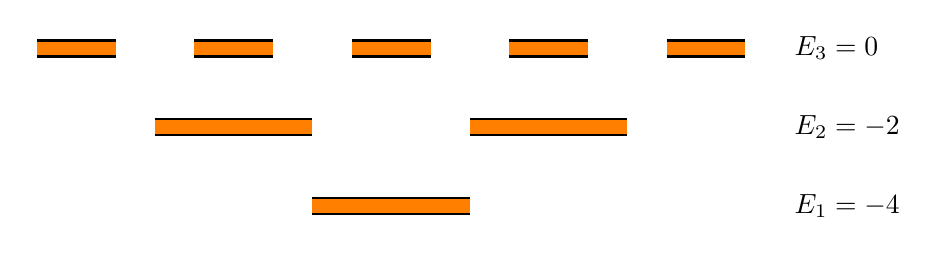
\begin{tikzpicture}
    \tikzset{level/.style   = {thick,
        double          = orange,
        double distance = 5pt,
        scale = 1.
        }}
    
    \def\Espace{9};
    \def\Gspace{11};
    
    % Draw the energy levels.
    \draw[level] (3,0)  -- (5,0) node[right]{};
    \draw[] (\Espace,0) node[right] {$E_1=-4$};
   
    \draw[level] (1,1) -- (3,1) node[right] {};
    \draw[level] (5,1) -- (7,1) node[right] {};
    \draw[] (\Espace,1) node[right] {$E_2=-2$};
    
    \def\v{.5}; 
    \draw[level] (-1+\v,2) -- (0+\v,2) node[right] {};
    \draw[level] (1+\v,2) -- (2+\v,2) node[right] {};
    \draw[level] (3+\v,2) -- (4+\v,2) node[right] {};
    \draw[level] (5+\v,2) -- (6+\v,2) node[right] {};
    \draw[level] (7+\v,2) -- (8+\v,2) node[right] {};
    \draw[] (\Espace,2) node[right] {$E_3=0$};
  \end{tikzpicture}
}


\newcommand{\TIKZgraphABC}{
  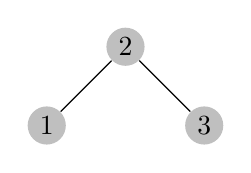
\begin{tikzpicture}[shorten >=1pt,->]
    \tikzstyle{vertex}=[circle,fill=black!25,minimum size=12pt,inner sep=2pt]
    \node[vertex] (G_1) at (-1,-1) {1};
    \node[vertex] (G_2) at (0,0)   {2};
    \node[vertex] (G_3) at (1,-1)  {3};
    \draw (G_1) -- (G_2) -- (G_3) -- cycle;
  \end{tikzpicture}
}

\newcommand{\TIKZgraphAB}{
  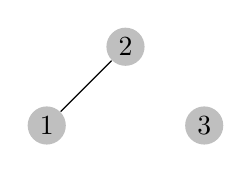
\begin{tikzpicture}[shorten >=1pt,->]
    \tikzstyle{vertex}=[circle,fill=black!25,minimum size=12pt,inner sep=2pt]
    \node[vertex] (G_1) at (-1,-1) {1};
    \node[vertex] (G_2) at (0,0)   {2};
    \node[vertex] (G_3) at (1,-1)  {3};
    \draw (G_1) -- (G_2) -- cycle;
  \end{tikzpicture}
}

\newcommand{\TIKZgraphBC}{
  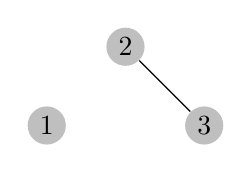
\begin{tikzpicture}[shorten >=1pt,->]
    \tikzstyle{vertex}=[circle,fill=black!25,minimum size=12pt,inner sep=2pt]
    \node[vertex] (G_1) at (-1,-1) {1};
    \node[vertex] (G_2) at (0,0)   {2};
    \node[vertex] (G_3) at (1,-1)  {3};
    \draw (G_2) -- (G_3) -- cycle;
  \end{tikzpicture}
}

\newcommand{\TIKZgraphC}{
  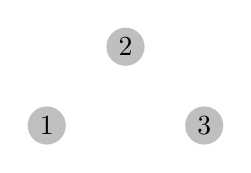
\begin{tikzpicture}[shorten >=1pt,->]
    \tikzstyle{vertex}=[circle,fill=black!25,minimum size=12pt,inner sep=2pt]
    \node[vertex] (G_1) at (-1,-1) {1};
    \node[vertex] (G_2) at (0,0)   {2};
    \node[vertex] (G_3) at (1,-1)  {3};
  \end{tikzpicture}
}


\newcommand{\TIKZgraphoneline}{
  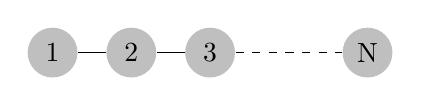
\begin{tikzpicture}[shorten >=1pt,->]
    \tikzstyle{vertex}=[circle,fill=black!25,minimum size=18pt,inner sep=2pt]
    \node[vertex] (G1) at (0,0)   {1};
    \node[vertex] (G2) at (1,0)   {2};
    \node[vertex] (G3) at (2,0)   {3};
    \node[vertex] (GN) at (4,0)   {N};
    \draw (G1) -- (G2) -- (G3) -- cycle;
    \draw[dashed] (G3) -- (GN) -- cycle;
  \end{tikzpicture}
}


\newcommand{\TIKZgraphtwoline}{
  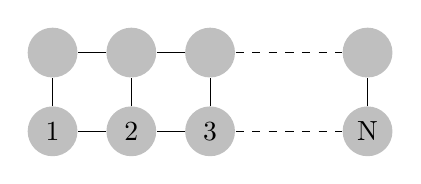
\begin{tikzpicture}[shorten >=1pt,->]
    \tikzstyle{vertex}=[circle,fill=black!25,minimum size=18pt,inner sep=2pt]
    \node[vertex] (G1) at (0,0)   {1};
    \node[vertex] (G2) at (1,0)   {2};
    \node[vertex] (G3) at (2,0)   {3};
    \node[vertex] (GN) at (4,0)   {N};
    \draw (G1) -- (G2) -- (G3) -- cycle;
    \draw[dashed] (G3) -- (GN) -- cycle;

    \node[vertex] (GN1) at (0,1)   {};
    \node[vertex] (GN2) at (1,1)   {};
    \node[vertex] (GN3) at (2,1)   {};
    \node[vertex] (G2N) at (4,1)   {};
    
    \draw (GN1) -- (GN2) -- (GN3) -- cycle;
    \draw (GN) -- (G2N) -- cycle;
    \draw (G1) -- (GN1) -- cycle;
    \draw (G2) -- (GN2) -- cycle;
    \draw (G3) -- (GN3) -- cycle;
    \draw (GN) -- (G2N) -- cycle;

    \draw[dashed] (GN3) -- (G2N) -- cycle;


  \end{tikzpicture}
}



\newcommand{\TIKZtwoladdera}{
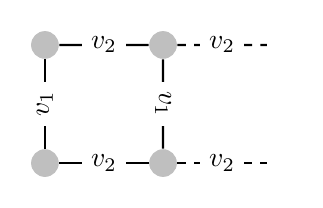
\begin{tikzpicture}[scale=\tikzpicscale]
    \node[vertex] (G1) at (0,0)   {};
    \node[vertex] (G2) at (1,0)   {};
    \node[vertex] (GA) at (0,1)   {};
    \node[vertex] (GB) at (1,1)   {};
	 \Edge[label=$v_2$](G1)(G2)
	 \Edge[label=$v_2$](GA)(GB)
	 \Edge[label=$v_1$](G1)(GA)
	 \Edge[label=$v_1$](G2)(GB)
    \node[Nvertex] (G3) at (2,0)   {};
    \node[Nvertex] (GC) at (2,1)   {};
	 \tikzstyle{EdgeStyle}=[dashed]
	 \Edge[label=$v_2$](G2)(G3)
	 \Edge[label=$v_2$](GB)(GC)
\end{tikzpicture}
}

\newcommand{\TIKZtwoladderb}{
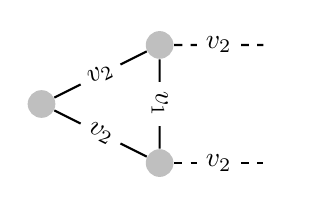
\begin{tikzpicture}[scale=\tikzpicscale]
    \node[vertex] (G2) at (1,0)   {};
    \node[vertex] (GB) at (1,1)   {};
    \node[vertex] (G1A) at (0,.5)   {};
	 \Edge[label=$v_2$](G1A)(G2)
	 \Edge[label=$v_2$](G1A)(GB)
	 \Edge[label=$v_1$](G2)(GB)
    \node[Nvertex] (G3) at (2,0)   {};
    \node[Nvertex] (GC) at (2,1)   {};
	 \tikzstyle{EdgeStyle}=[dashed]
	 \Edge[label=$v_2$](G2)(G3)
	 \Edge[label=$v_2$](GB)(GC)
\end{tikzpicture}
}

\newcommand{\TIKZtwoladderc}{
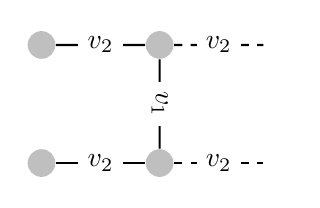
\begin{tikzpicture}[scale=\tikzpicscale]
    \node[vertex] (G1) at (0,0)   {};
    \node[vertex] (G2) at (1,0)   {};
    \node[vertex] (GA) at (0,1)   {};
    \node[vertex] (GB) at (1,1)   {};
	 \Edge[label=$v_2$](G1)(G2)
	 \Edge[label=$v_2$](GA)(GB)
	 %\Edge[label=$v_1$](G1)(GA)
	 \Edge[label=$v_1$](G2)(GB)
    \node[Nvertex] (G3) at (2,0)   {};
    \node[Nvertex] (GC) at (2,1)   {};
	 \tikzstyle{EdgeStyle}=[dashed]
	 \Edge[label=$v_2$](G2)(G3)
	 \Edge[label=$v_2$](GB)(GC)
\end{tikzpicture}
}

\newcommand{\TIKZtwoladderd}{
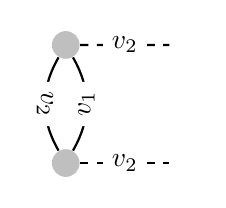
\begin{tikzpicture}[scale=\tikzpicscale]
    \node[vertex] (G2) at (1,0)   {};
    \node[vertex] (GB) at (1,1)   {};
	 %\Edge[label=$v_1$](G1)(GA)
	\tikzstyle{EdgeStyle}=[bend left]
	\Edge[label=$v_2$](G2)(GB)
  	\tikzstyle{EdgeStyle}=[bend right]
	\Edge[label=$v_1$](G2)(GB)
    \node[Nvertex] (G3) at (2,0)   {};
    \node[Nvertex] (GC) at (2,1)   {};
	 \tikzstyle{EdgeStyle}=[dashed]
	 \Edge[label=$v_2$](G2)(G3)
	 \Edge[label=$v_2$](GB)(GC)
\end{tikzpicture}
}

\newcommand{\TIKZtwoladdere}{
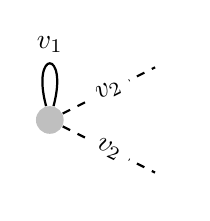
\begin{tikzpicture}[scale=\tikzpicscale]
    \node[vertex] (G2B) at (1,.5)   {};
	 %\Edge[label=$v_1$](G1)(GA)
	\tikzstyle{EdgeStyle}=[loop above]
	\Edge[label=$v_1$](G2B)(G2B)
   \node[Nvertex] (G3) at (2,0)   {};
   \node[Nvertex] (GC) at (2,1)   {};
	\tikzstyle{EdgeStyle}=[dashed]
	\Edge[label=$v_2$](G2B)(G3)
	\Edge[label=$v_2$](G2B)(GC)
\end{tikzpicture}
}

\newcommand{\TIKZtwoladderf}{
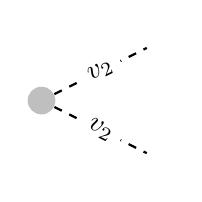
\begin{tikzpicture}[scale=\tikzpicscale]
    \node[vertex] (G2B) at (1,.5)   {};
   \node[Nvertex] (G3) at (2,0)   {};
   \node[Nvertex] (GC) at (2,1)   {};
	\tikzstyle{EdgeStyle}=[dashed]
	\Edge[label=$v_2$](G2B)(G3)
	\Edge[label=$v_2$](G2B)(GC)
\end{tikzpicture}
}

\newcommand{\TIKZthreeladderA}{
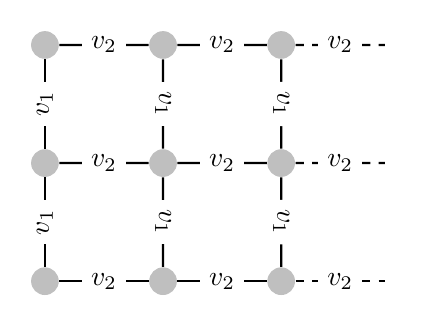
\begin{tikzpicture}[scale=\tikzpicscale]
    \node[vertex] (00) at (0,0)   {};
    \node[vertex] (10) at (1,0)   {};
	 \node[vertex] (20) at (2,0)   {};
    \node[vertex] (01) at (0,1)   {};
    \node[vertex] (11) at (1,1)   {};
    \node[vertex] (21) at (2,1)   {};
    \node[vertex] (02) at (0,2)   {};
    \node[vertex] (12) at (1,2)   {};
    \node[vertex] (22) at (2,2)   {};
	 \Edge[label=$v_2$](00)(10)
	 \Edge[label=$v_2$](10)(20)
	 \Edge[label=$v_2$](01)(11)
	 \Edge[label=$v_2$](11)(21)
	 \Edge[label=$v_2$](02)(12)
	 \Edge[label=$v_2$](12)(22)	
	 \Edge[label=$v_1$](00)(01)
	 \Edge[label=$v_1$](10)(11)
	 \Edge[label=$v_1$](20)(21)
 	 \Edge[label=$v_1$](21)(22)
 	 \Edge[label=$v_1$](11)(12)
 	 \Edge[label=$v_1$](01)(02)
    \node[Nvertex] (n30) at (3,0)   {};
    \node[Nvertex] (n31) at (3,1)   {};
    \node[Nvertex] (n32) at (3,2)   {};
	 \tikzstyle{EdgeStyle}=[dashed]
	 \Edge[label=$v_2$](20)(n30)
	 \Edge[label=$v_2$](21)(n31)
 	 \Edge[label=$v_2$](22)(n32)
\end{tikzpicture}
}

\newcommand{\TIKZthreeladderB}{
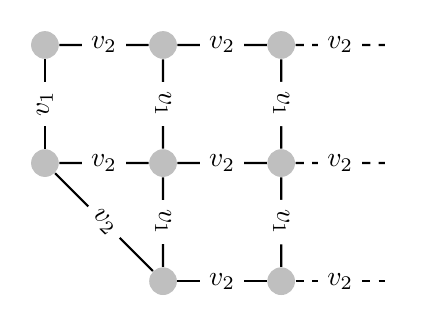
\begin{tikzpicture}[scale=\tikzpicscale]
%    \node[vertex] (00) at (0,0)   {};
    \node[vertex] (10) at (1,0)   {};
	 \node[vertex] (20) at (2,0)   {};
    \node[vertex] (01) at (0,1)   {};
    \node[vertex] (11) at (1,1)   {};
    \node[vertex] (21) at (2,1)   {};
    \node[vertex] (02) at (0,2)   {};
    \node[vertex] (12) at (1,2)   {};
    \node[vertex] (22) at (2,2)   {};
	 \Edge[label=$v_2$](01)(10)
	 \Edge[label=$v_2$](10)(20)
	 \Edge[label=$v_2$](01)(11)
	 \Edge[label=$v_2$](11)(21)
	 \Edge[label=$v_2$](02)(12)
	 \Edge[label=$v_2$](12)(22)	
%)	 \Edge[label=$v_1$](00)(01)
	 \Edge[label=$v_1$](10)(11)
	 \Edge[label=$v_1$](20)(21)
 	 \Edge[label=$v_1$](21)(22)
 	 \Edge[label=$v_1$](11)(12)
 	 \Edge[label=$v_1$](01)(02)
    \node[Nvertex] (n30) at (3,0)   {};
    \node[Nvertex] (n31) at (3,1)   {};
    \node[Nvertex] (n32) at (3,2)   {};
	 \tikzstyle{EdgeStyle}=[dashed]
	 \Edge[label=$v_2$](20)(n30)
	 \Edge[label=$v_2$](21)(n31)
 	 \Edge[label=$v_2$](22)(n32)
\end{tikzpicture}
}

\newcommand{\TIKZthreeladderC}{
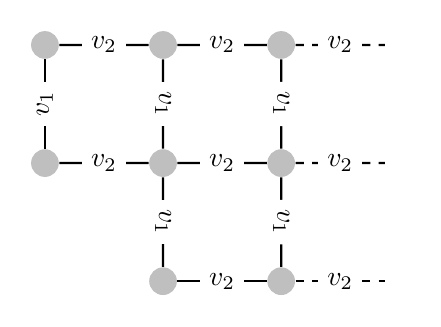
\begin{tikzpicture}[scale=\tikzpicscale]
%    \node[vertex] (00) at (0,0)   {};
    \node[vertex] (10) at (1,0)   {};
	 \node[vertex] (20) at (2,0)   {};
    \node[vertex] (01) at (0,1)   {};
    \node[vertex] (11) at (1,1)   {};
    \node[vertex] (21) at (2,1)   {};
    \node[vertex] (02) at (0,2)   {};
    \node[vertex] (12) at (1,2)   {};
    \node[vertex] (22) at (2,2)   {};
%	 \Edge[label=$v_2$](01)(10)
	 \Edge[label=$v_2$](10)(20)
	 \Edge[label=$v_2$](01)(11)
	 \Edge[label=$v_2$](11)(21)
	 \Edge[label=$v_2$](02)(12)
	 \Edge[label=$v_2$](12)(22)	
%)	 \Edge[label=$v_1$](00)(01)
	 \Edge[label=$v_1$](10)(11)
	 \Edge[label=$v_1$](20)(21)
 	 \Edge[label=$v_1$](21)(22)
 	 \Edge[label=$v_1$](11)(12)
 	 \Edge[label=$v_1$](01)(02)
    \node[Nvertex] (n30) at (3,0)   {};
    \node[Nvertex] (n31) at (3,1)   {};
    \node[Nvertex] (n32) at (3,2)   {};
	 \tikzstyle{EdgeStyle}=[dashed]
	 \Edge[label=$v_2$](20)(n30)
	 \Edge[label=$v_2$](21)(n31)
 	 \Edge[label=$v_2$](22)(n32)
\end{tikzpicture}
}

\newcommand{\TIKZthreeladderD}{
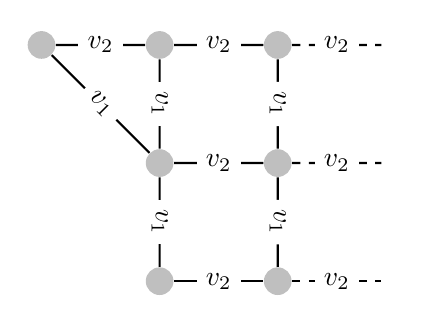
\begin{tikzpicture}[scale=\tikzpicscale]
%    \node[vertex] (00) at (0,0)   {};
    \node[vertex] (10) at (1,0)   {};
	 \node[vertex] (20) at (2,0)   {};
%    \node[vertex] (01) at (0,1)   {};
    \node[vertex] (11) at (1,1)   {};
    \node[vertex] (21) at (2,1)   {};
    \node[vertex] (02) at (0,2)   {};
    \node[vertex] (12) at (1,2)   {};
    \node[vertex] (22) at (2,2)   {};
%	 \Edge[label=$v_2$](01)(10)
	 \Edge[label=$v_2$](10)(20)
%	 \Edge[label=$v_2$](01)(11)
	 \Edge[label=$v_2$](11)(21)
	 \Edge[label=$v_2$](02)(12)
	 \Edge[label=$v_2$](12)(22)	
%)	 \Edge[label=$v_1$](00)(01)
	 \Edge[label=$v_1$](10)(11)
	 \Edge[label=$v_1$](20)(21)
 	 \Edge[label=$v_1$](21)(22)
 	 \Edge[label=$v_1$](11)(12)
 	 \Edge[label=$v_1$](11)(02)
    \node[Nvertex] (n30) at (3,0)   {};
    \node[Nvertex] (n31) at (3,1)   {};
    \node[Nvertex] (n32) at (3,2)   {};
	 \tikzstyle{EdgeStyle}=[dashed]
	 \Edge[label=$v_2$](20)(n30)
	 \Edge[label=$v_2$](21)(n31)
 	 \Edge[label=$v_2$](22)(n32)
\end{tikzpicture}
}

\newcommand{\TIKZthreeladderE}{
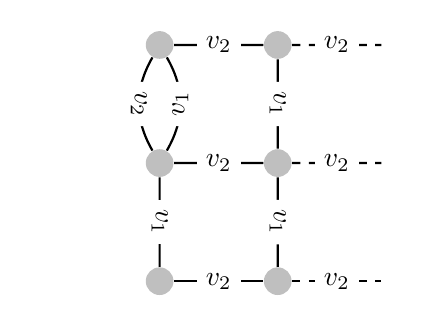
\begin{tikzpicture}[scale=\tikzpicscale]
    \node[Nvertex] (00) at (0,0)   {};
    \node[vertex] (10) at (1,0)   {};
	 \node[vertex] (20) at (2,0)   {};
%    \node[vertex] (01) at (0,1)   {};
    \node[vertex] (11) at (1,1)   {};
    \node[vertex] (21) at (2,1)   {};
%    \node[vertex] (02) at (0,2)   {};
    \node[vertex] (12) at (1,2)   {};
    \node[vertex] (22) at (2,2)   {};
%	 \Edge[label=$v_2$](01)(10)
	 \Edge[label=$v_2$](10)(20)
%	 \Edge[label=$v_2$](01)(11)
	 \Edge[label=$v_2$](11)(21)
%	 \Edge[label=$v_2$](02)(12)
	 \Edge[label=$v_2$](12)(22)	
%)	 \Edge[label=$v_1$](00)(01)
	 \Edge[label=$v_1$](10)(11)
	 \Edge[label=$v_1$](20)(21)
 	 \Edge[label=$v_1$](21)(22)
% 	 \Edge[label=$v_1$](11)(02)
    \node[Nvertex] (n30) at (3,0)   {};
    \node[Nvertex] (n31) at (3,1)   {};
    \node[Nvertex] (n32) at (3,2)   {};
	 \tikzstyle{EdgeStyle}=[dashed]
	 \Edge[label=$v_2$](20)(n30)
	 \Edge[label=$v_2$](21)(n31)
 	 \Edge[label=$v_2$](22)(n32)
 	 \tikzstyle{EdgeStyle}=[bend left]
  	 \Edge[label=$v_2$](11)(12)
  	 \tikzstyle{EdgeStyle}=[bend right]
  	 \Edge[label=$v_1$](11)(12)
\end{tikzpicture}
}

\newcommand{\TIKZthreeladderF}{
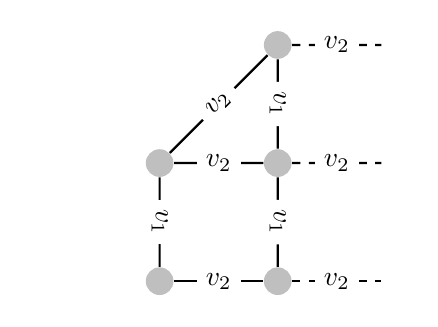
\begin{tikzpicture}[scale=\tikzpicscale]
    \node[Nvertex] (00) at (0,0)   {};
    \node[vertex] (10) at (1,0)   {};
	 \node[vertex] (20) at (2,0)   {};
%    \node[vertex] (01) at (0,1)   {};
    \node[vertex] (11) at (1,1)   {};
    \node[vertex] (21) at (2,1)   {};
%    \node[vertex] (02) at (0,2)   {};
%    \node[vertex] (12) at (1,2)   {};
    \node[vertex] (22) at (2,2)   {};
%	 \Edge[label=$v_2$](01)(10)
	 \Edge[label=$v_2$](10)(20)
%	 \Edge[label=$v_2$](01)(11)
	 \Edge[label=$v_2$](11)(21)
%	 \Edge[label=$v_2$](02)(12)
	 \Edge[label=$v_2$](11)(22)	
%)	 \Edge[label=$v_1$](00)(01)
	 \Edge[label=$v_1$](10)(11)
	 \Edge[label=$v_1$](20)(21)
 	 \Edge[label=$v_1$](21)(22)
% 	 \Edge[label=$v_1$](11)(02)
    \node[Nvertex] (n30) at (3,0)   {};
    \node[Nvertex] (n31) at (3,1)   {};
    \node[Nvertex] (n32) at (3,2)   {};
	 \tikzstyle{EdgeStyle}=[dashed]
	 \Edge[label=$v_2$](20)(n30)
	 \Edge[label=$v_2$](21)(n31)
 	 \Edge[label=$v_2$](22)(n32)
  	 %\tikzstyle{EdgeStyle}=[loop above]
  	 %\Edge[label=$v_1$](11)(11)
\end{tikzpicture}
}

\newcommand{\TIKZthreeladderG}{
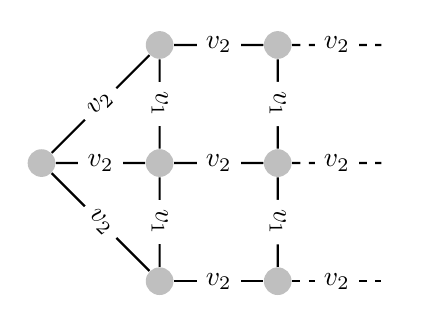
\begin{tikzpicture}[scale=\tikzpicscale]
%    \node[vertex] (00) at (0,0)   {};
    \node[vertex] (10) at (1,0)   {};
	 \node[vertex] (20) at (2,0)   {};
    \node[vertex] (01) at (0,1)   {};
    \node[vertex] (11) at (1,1)   {};
    \node[vertex] (21) at (2,1)   {};
%    \node[vertex] (02) at (0,2)   {};
    \node[vertex] (12) at (1,2)   {};
    \node[vertex] (22) at (2,2)   {};
	 \Edge[label=$v_2$](01)(10)
	 \Edge[label=$v_2$](10)(20)
	 \Edge[label=$v_2$](01)(11)
	 \Edge[label=$v_2$](11)(21)
	 \Edge[label=$v_2$](01)(12)
	 \Edge[label=$v_2$](12)(22)	
%)	 \Edge[label=$v_1$](00)(01)
	 \Edge[label=$v_1$](10)(11)
	 \Edge[label=$v_1$](20)(21)
 	 \Edge[label=$v_1$](21)(22)
 	 \Edge[label=$v_1$](11)(12)
% 	 \Edge[label=$v_1$](01)(02)
    \node[Nvertex] (n30) at (3,0)   {};
    \node[Nvertex] (n31) at (3,1)   {};
    \node[Nvertex] (n32) at (3,2)   {};
	 \tikzstyle{EdgeStyle}=[dashed]
	 \Edge[label=$v_2$](20)(n30)
	 \Edge[label=$v_2$](21)(n31)
 	 \Edge[label=$v_2$](22)(n32)
\end{tikzpicture}
}

\newcommand{\TIKZthreeladderH}{
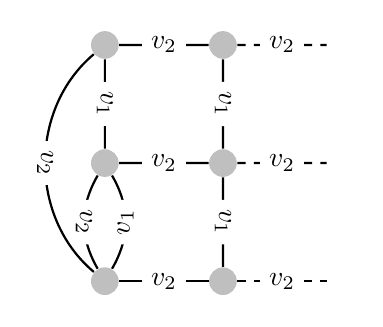
\begin{tikzpicture}[scale=\tikzpicscale]
%    \node[vertex] (00) at (0,0)   {};
    \node[vertex] (10) at (1,0)   {};
	 \node[vertex] (20) at (2,0)   {};
%    \node[vertex] (01) at (0,1)   {};
    \node[vertex] (11) at (1,1)   {};
    \node[vertex] (21) at (2,1)   {};
%    \node[vertex] (02) at (0,2)   {};
    \node[vertex] (12) at (1,2)   {};
    \node[vertex] (22) at (2,2)   {};
	 \Edge[label=$v_2$](10)(20)
%	 \Edge[label=$v_2$](01)(11)
	 \Edge[label=$v_2$](11)(21)
%	 \Edge[label=$v_2$](01)(12)
	 \Edge[label=$v_2$](12)(22)	
%)	 \Edge[label=$v_1$](00)(01)
	 \Edge[label=$v_1$](20)(21)
 	 \Edge[label=$v_1$](21)(22)
 	 \Edge[label=$v_1$](11)(12)
% 	 \Edge[label=$v_1$](01)(02)
    \node[Nvertex] (n30) at (3,0)   {};
    \node[Nvertex] (n31) at (3,1)   {};
    \node[Nvertex] (n32) at (3,2)   {};
	 \tikzstyle{EdgeStyle}=[dashed]
	 \Edge[label=$v_2$](20)(n30)
	 \Edge[label=$v_2$](21)(n31)
 	 \Edge[label=$v_2$](22)(n32)
 	 
 	 \tikzstyle{EdgeStyle}=[bend left]
 	 \Edge[label=$v_2$](10)(11)
  	 \tikzstyle{EdgeStyle}=[bend left=50]
 	 \Edge[label=$v_2$](10)(12)
  	 %\Edge[label=$v_2$](11)(12)
 	 \tikzstyle{EdgeStyle}=[bend right]
	 \Edge[label=$v_1$](10)(11)
\end{tikzpicture}
}

\newcommand{\TIKZthreeladderI}{
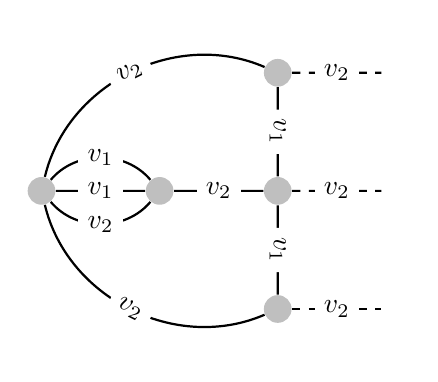
\begin{tikzpicture}[scale=\tikzpicscale]
%    \node[vertex] (00) at (0,0)   {};
%    \node[vertex] (10) at (1,0)   {};
	 \node[vertex] (20) at (2,0)   {};
    \node[vertex] (01) at (0,1)   {};
    \node[vertex] (11) at (1,1)   {};
    \node[vertex] (21) at (2,1)   {};
%    \node[vertex] (02) at (0,2)   {};
%    \node[vertex] (12) at (1,2)   {};
    \node[vertex] (22) at (2,2)   {};
%	 \Edge[label=$v_2$](01)(10)
%	 \Edge[label=$v_2$](10)(20)
%	 \Edge[label=$v_2$](01)(21)
	 \Edge[label=$v_2$](11)(21)
%	 \Edge[label=$v_2$](12)(22)	
%)	 \Edge[label=$v_1$](00)(01)
%	 \Edge[label=$v_1$](10)(11)
	 \Edge[label=$v_1$](20)(21)
 	 \Edge[label=$v_1$](21)(22)
% 	 \Edge[label=$v_1$](11)(12)
% 	 \Edge[label=$v_1$](01)(02)
    \node[Nvertex] (n30) at (3,0)   {};
    \node[Nvertex] (n31) at (3,1)   {};
    \node[Nvertex] (n32) at (3,2)   {};
	 \tikzstyle{EdgeStyle}=[dashed]
	 \Edge[label=$v_2$](20)(n30)
	 \Edge[label=$v_2$](21)(n31)
 	 \Edge[label=$v_2$](22)(n32)

	 \tikzstyle{EdgeStyle}=[]
	 \Edge[label=$v_1$](01)(11)
  	 \tikzstyle{EdgeStyle}=[bend left=50]
	 \Edge[label=$v_2$](01)(22)
 	 \Edge[label=$v_1$](01)(11)
  	 \tikzstyle{EdgeStyle}=[bend right=50]
 	 \Edge[label=$v_2$](01)(20)
 	 \Edge[label=$v_2$](01)(11)
\end{tikzpicture}
}


\newcommand{\TIKZthreeladderJ}{
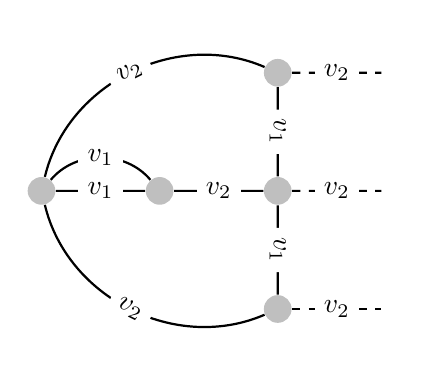
\begin{tikzpicture}[scale=\tikzpicscale]
%    \node[vertex] (00) at (0,0)   {};
%    \node[vertex] (10) at (1,0)   {};
	 \node[vertex] (20) at (2,0)   {};
    \node[vertex] (01) at (0,1)   {};
    \node[vertex] (11) at (1,1)   {};
    \node[vertex] (21) at (2,1)   {};
%    \node[vertex] (02) at (0,2)   {};
%    \node[vertex] (12) at (1,2)   {};
    \node[vertex] (22) at (2,2)   {};
%	 \Edge[label=$v_2$](01)(10)
%	 \Edge[label=$v_2$](10)(20)
%	 \Edge[label=$v_2$](01)(21)
	 \Edge[label=$v_2$](11)(21)
%	 \Edge[label=$v_2$](12)(22)	
%)	 \Edge[label=$v_1$](00)(01)
%	 \Edge[label=$v_1$](10)(11)
	 \Edge[label=$v_1$](20)(21)
 	 \Edge[label=$v_1$](21)(22)
% 	 \Edge[label=$v_1$](11)(12)
% 	 \Edge[label=$v_1$](01)(02)
    \node[Nvertex] (n30) at (3,0)   {};
    \node[Nvertex] (n31) at (3,1)   {};
    \node[Nvertex] (n32) at (3,2)   {};
	 \tikzstyle{EdgeStyle}=[dashed]
	 \Edge[label=$v_2$](20)(n30)
	 \Edge[label=$v_2$](21)(n31)
 	 \Edge[label=$v_2$](22)(n32)

	 \tikzstyle{EdgeStyle}=[]
	 \Edge[label=$v_1$](01)(11)
  	 \tikzstyle{EdgeStyle}=[bend left=50]
	 \Edge[label=$v_2$](01)(22)
 	 \Edge[label=$v_1$](01)(11)
  	 \tikzstyle{EdgeStyle}=[bend right=50]
 	 \Edge[label=$v_2$](01)(20)
% 	 \Edge[label=$v_2$](01)(11)
\end{tikzpicture}
}

\newcommand{\TIKZoneladderA}{
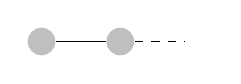
\begin{tikzpicture}[shorten >=1pt,->]
    \tikzstyle{vertex}=[circle,fill=black!25,minimum size=10pt,inner sep=2pt]
    \tikzstyle{nullvertex}=[circle,fill=white!25,minimum size=10pt,inner sep=2pt]
    \node[vertex] (G1) at (0,0)   {};
    \node[vertex] (G2) at (1,0)   {};
    \node[nullvertex] (GX) at (2,0)   {};
    \draw (G1) -- (G2) -- cycle;
    \draw[dashed] (G2) -- (GX) -- cycle;
\end{tikzpicture}
}

\newcommand{\TIKZoneladderB}{
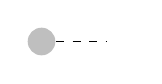
\begin{tikzpicture}[shorten >=1pt,->]
    \tikzstyle{vertex}=[circle,fill=black!25,minimum size=10pt,inner sep=2pt]
    \tikzstyle{nullvertex}=[circle,fill=white!25,minimum size=10pt,inner sep=2pt]
    \node[vertex] (G2) at (1,0)   {};
    \node[nullvertex] (GX) at (2,0)   {};
    \draw[dashed] (G2) -- (GX) -- cycle;
\end{tikzpicture}
}

\newcommand{\TIKZoneladderC}{

\begin{tikzpicture}[shorten >=1pt,->]
    \tikzstyle{vertex}=[circle,fill=black!25,minimum size=10pt,inner sep=2pt]
    \tikzstyle{nullvertex}=[circle,fill=white!25,minimum size=10pt,inner sep=2pt]
    \node[vertex] (G1) at (0,0)   {};
    \node[vertex] (G2) at (1,0)   {};
    \node[nullvertex] (GX) at (2,0)   {};
    %\draw (G1) -- (G2) -- cycle;
    \draw[dashed] (G2) -- (GX) -- cycle;
\end{tikzpicture}
}

\newcommand{\TIKZpetersengraph} {
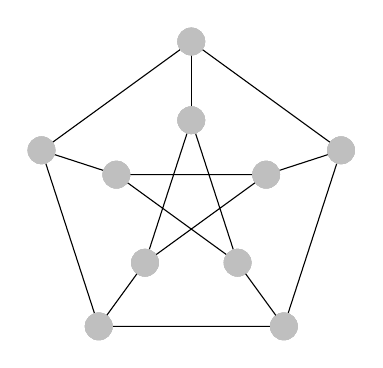
\begin{tikzpicture}[]
    \tikzstyle{vertex}=[circle,fill=black!25,minimum size=10pt,inner sep=2pt]
            
\draw (18:2cm) -- (90:2cm) -- (162:2cm) -- (234:2cm) -- (306:2cm) -- cycle;
\draw (18:1cm) -- (162:1cm) -- (306:1cm) -- (90:1cm) -- (234:1cm) -- cycle;
\foreach \x in {18,90,162,234,306}{
\draw (\x:1cm) -- (\x:2cm);

    \node[vertex] at (18:2cm) {};
    \node[vertex] at (90:2cm) {};
    \node[vertex] at (162:2cm) {};
    \node[vertex] at (234:2cm) {};
    \node[vertex] at (306:2cm) {};
    \node[vertex] at (18:1cm) {};
    \node[vertex] at (162:1cm) {};
    \node[vertex] at (306:1cm) {};
    \node[vertex] at (90:1cm) {};
    \node[vertex] at (234:1cm) {};

%\draw (\x:2cm) circle (2pt);
%\draw (\x:1cm) circle (2pt);
}
\end{tikzpicture}
}

\newcommand{\TIKZFLWmacrostates} {

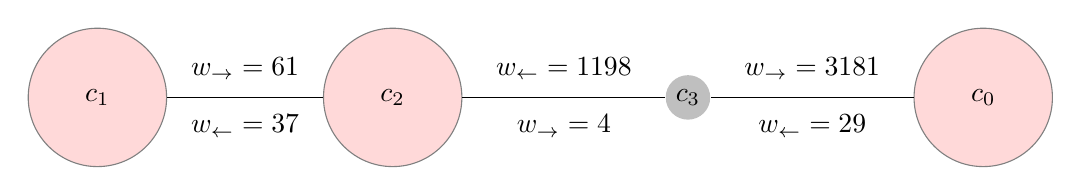
\begin{tikzpicture}[scale=\tikzpicscale]

  \node[big_vertex] (c1) at (0,0)   {$c_1$};
  \node[big_vertex] (c2) at (1*\vertexshiftamount,0)   {$c_2$};
  \node[vertex]    (c3) at (2*\vertexshiftamount,0)   {$c_3$};
  \node[big_vertex] (c0) at (3*\vertexshiftamount,0)   {$c_0$};
  
  \draw [] (c0) -> node[above=.1cm] {$w_{\rightarrow}=3181$} (c3);
  \draw [] (c0) -> node[below=.1cm] {$w_{\leftarrow}=29$} (c3);

  \draw [] (c2) -> node[above=.1cm] {$w_{\leftarrow}=1198$} (c3);  
  \draw [] (c2) -> node[below=.1cm] {$w_{\rightarrow}=4$} (c3);
  
  \draw [] (c2) -- node[below=.1cm] {$w_{\leftarrow}=37$} (c1);
  \draw [] (c2) -- node[above=.1cm] {$w_{\rightarrow}=61$} (c1);
\end{tikzpicture}
}

\newcommand{\TIKZbetahairpinNativestate} {
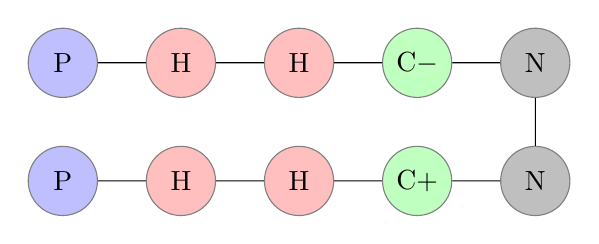
\begin{tikzpicture}[scale=\tikzpicscale]
    \tikzstyle{hvertex}=[circle,fill=red!25,minimum size=25pt,inner sep=2pt,draw=black!50]
    \tikzstyle{pvertex}=[circle,fill=blue!25,minimum size=25pt,inner sep=2pt,draw=black!50]
    \tikzstyle{cpvertex}=[circle,fill=green!25,minimum size=25pt,inner sep=2pt,draw=black!50]
    \tikzstyle{nvertex}=[circle,fill=black!25,minimum size=25pt,inner sep=2pt,draw=black!50]

    \node[pvertex] (r0) at (0,0)   {\chem{P}};
    \node[hvertex] (r1) at (1,0)   {\chem{H}};
    \node[hvertex] (r2) at (2,0)   {\chem{H}};
    \node[cpvertex] (r3) at (3,0)   {\chem{C+}};
    \node[nvertex] (r4) at (4,0)   {\chem{N}};
    \node[nvertex] (r5) at (4,1)   {\chem{N}};
    \node[cpvertex] (r6) at (3,1)   {\chem{C-}};
    \node[hvertex] (r7) at (2,1)   {\chem{H}};
    \node[hvertex] (r8) at (1,1)   {\chem{H}};
    \node[pvertex] (r9) at (0,1)   {\chem{P}};

    \draw [] (r0)--(r1)--(r2)--(r3)--(r4)--(r5)--(r6)--(r7)--(r8)--(r9)--cycle;
   
\end{tikzpicture}
}


\newcommand{\TIKZbetahairpinMacrostates} {
\begin{tikzpicture}[scale=\tikzpicscale]
    \node[macrostate_vertex] (R) at (0,0)   {
    \begin{minipage}{3.1cm}
    \includegraphics[width=1.5 cm]{supplement/beta_cluster_example_2/pictures/21/state_cluster_shapes_150.pdf} 
    \includegraphics[width=1.5 cm]{supplement/beta_cluster_example_2/pictures/21/state_cluster_shapes_17.pdf} \\
    \includegraphics[width=1.5 cm]{supplement/beta_cluster_example_2/pictures/21/state_cluster_shapes_32.pdf} 
    \includegraphics[width=1.5 cm]{supplement/beta_cluster_example_2/pictures/21/state_cluster_shapes_200.pdf} \\
  	 $c_\chem{R}$ random coil
    \end{minipage}
    };
    \node[macrostate_vertex] (I) at (1.5*\vertexshiftamount,0)   {
    \begin{minipage}{3.1cm} \centering
    \includegraphics[width=2 cm]{supplement/beta_cluster_example_2/pictures/saved_macrostates/intermed.png} \\
  	 $c_\chem{I}$ intermediate \\ (turn formation)
    \end{minipage}
	 };
    \node[macrostate_vertex] (F) at (3*\vertexshiftamount,0)   
    {
    \begin{minipage}{3.1cm} \centering
    \includegraphics[width=2.5 cm]{supplement/beta_cluster_example_2/pictures/saved_macrostates/native.png} \\
  	 $c_\chem{F}$ native state
    \end{minipage}
    };

  \tikzstyle{EdgeStyle}=[bend right]
  \Edge[label=$\B{S}_{\chem{R I}}$](R)(I)
  \Edge[label=$\B{S}_{\chem{I R}}$](I)(R)
  
  \tikzstyle{EdgeStyle}=[]
  \Edge[label=$\B{S}_{\chem{I F}}$](I)(F)
  
\end{tikzpicture}
}


%\end{comment}



\begin{document}


\suppressfooter
\begin{preamble}

\iffinal{}{\newpage}
\begin{DUTdedications}
%
\vspace*{\fill}
%
\begin{center}
\setstretch{2}
\begin{minipage}{8 cm}
\begin{center}
\hrulefill\\
This thesis is dedicated to Cara Hoppe.\\ 
I respect her as my peer,\\
and cherish her as my wife.\\
Her love and support made this work possible. \\
%\hrulefill\hspace{0.2cm} \leafNE \hspace{0.2cm} \hrulefill
\hrulefill
\vspace{6em}
\end{center}
\end{minipage}
\end{center} 
%
\vspace*{\fill}
%
\end{DUTdedications} 
\iffinal{}{\newpage}

\begin{acknowledgments}
  \iffinal{}{\setstretch{1.5}}
The completion of this thesis could not have been done without the tireless support of my advisor, Dr. Jian-Min Yuan. I am deeply indebted for the support he has provided over the years. As a mentor, he helped me develop my skills as a scientist and honed my critical thinking. He is an endless source of new ideas and has taught me how to effectively communicate in the scientific world. 

I would also like to thank the physics department at Drexel for helping me prepare for the journey ahead. In particular, both Dr. Michel Vallieres and Dr. Robert Gilmore have been gracious enough to spend many afternoons discussing every interesting theory I've come across. Their insights and enthusiasm for physics and mathematics is inspiring. 

I would like to thank my family, my wife, Cara Hoppe, and my children, Hazel and Jackson Hoppe. They cheerfully remind me of the world outside and always bring a smile to my face. Finally, I would like to thank my uncle, Fred Stein, who introduced me to physics and all its wonders at an early age.
 
  \end{acknowledgments}
  \iffinal{}{\newpage}

  \listoffigures 
  \iffinal{}{\newpage}

  \tableofcontents 
  \iffinal{}{\newpage}

  \begin{abstract}
  \iffinal{}{\setstretch{1.5}}
  \setstretch{1.5}
A protein's ultimate function and activity is determined by the unique three-dimensional structure taken by the folding process. Protein malfunction due to misfolding is the culprit of many clinical disorders, such as abnormal protein aggregations. This leads to neurodegenerative disorders like Huntington's and Alzheimer's disease. We focus on a subset of the folding problem, exploring the role and effects of entropy on the process of protein folding. Four major concepts and models are developed and each pertains to a specific aspect of the folding process: entropic forces, conformational states under crowding, aggregation, and macrostate kinetics from microstate trajectories. 

The exclusive focus on entropy is well-suited for crowding studies, as many interactions are non-specific. We show how a stabilizing entropic force can arise purely from the motion of crowders in solution. In addition we are able to make a a quantitative prediction of the crowding effect with an implicit crowding approximation using an aspherical scaled-particle theory.

In order to investigate the effects of aggregation, we derive a new operator expansion method to solve the Ising/Potts model with external fields over an arbitrary graph. Here the external fields are representative of the entropic forces. We show that this method reduces the problem of calculating the partition function to the solution of recursion relations. 

Many of the methods employed are coarse-grained approximations. As such, it is useful to have a viable method for extracting macrostate information from time series data. We develop a method to cluster the microstates into physically meaningful macrostates by grouping similar relaxation times from a transition matrix.  

Overall, the studied topics allow us to understand deeper the complicated process involving proteins.
  \end{abstract} 

	\iffinal{}{\newpage}

\end{preamble}


\begin{thesis}
  \pdfbookmark[-1]{Main Matter}{Main Matter}
  \setstretch{1.2}
  \chapter*{Preface}

\begin{comment}
  Throughout history, scientific fields have split, merged and been made obsolete. What we find important is dictated by our philosophical ideals, economic status, cultural norms and scientific curiosity. The current frontiers of science aim probe our understandings of the very laws of physics through our studies of the exotic Higgs boson to recreating the wistful alchemical dream of artificial atoms through quantum dots. Corporeally, we have staked out the biological form as new fertile ground for us explore and pioneer. The explosive growth in this interest, fueled by new technologies, has lead to the growth of a new multi-disciplined approach called biophysics.
\end{comment}

Traditionally, the components of biophysics, biology and physics, have a tangential mode of thought.  Biology, the study of living things, is a field governed by qualitative observation and later mathematical models are applied. Prediction comes from the understanding of the various mechanisms that are often intricately coupled. On the other hand, a mature branch of physics is governed by the mathematical form first. Ideas are founded from first principles, from which the physical laws are then derived. If these predictions fail to accurately portray reality the fundamental assumptions are discarded and presumed to be false. The successful theories in physics have a far greater precision than the biological counterparts. How then do the two fields reconcile, the dogma of each being so different?
%
\begin{equation*}
  \chem{bioPHYSICS \longleftrightarrow BIOphysics}
\end{equation*}

In this author’s opinion, the field of biophysics has truly made possible by a third kind of science. After experiment and theory comes modeling, an approach that has been greatly enhanced by the use of modern day computers. Scientific modeling incorporates rigorous mathematical derivations, yet the results are interpreted as though they were experimental evidence. It is rapidly being recognized as an important and vital component to our scientific endeavors.\cite{reed_computational_2005} In some ways modeling takes the best of both forms, allowing each to contribute. This approach has been used in many diverse fields such as meteorology, economics, and our present topic, biophysics.

Biophysics has an implicit scale. Usually the scale spans from collections of cells (on order of microns) to collections of atoms (on order of angstroms). As an example of the types of objects currently studied, Figure \ref{fig:conf_words} shows the usage of the words found in abstracts of presentations and posters at a recent biophysics conference. The three dominant objects that were studied were proteins, cells, and membranes. The larger structures (except in the cases of aggregation) traditionally studied in biology are out of the scope of most biophysical studies. 
%
\begin{figure}
  \begin{centering}
    \fbox{\includegraphics[height=5 cm]
      {pictures/wordcloud_conf/abstract_wordcloud.pdf}}
    \caption{Snapshot of the most commonly used words in the abstracts of the 2010 Biophysical Conference in San Francisco.\cite{BPS_conf_2010} Larger words correspond to a greater usage. Note that the prominent words, protein, cell, and membrane set the length scale that narrows the focus of the discipline.}
    \label{fig:conf_words}
  \end{centering}
\end{figure}

As we move to smaller structures we find ourselves in the realm of quantum chemistry and pure physics. In this regime, theories of ``first-principle'' abound. That is, starting from a set of empirically verified postulates, equations are derived which predict the dynamics and structure of the system. As we move to larger structures we are back in the traditional biological realm, where the role of classification dictates the functionality. 
For the theoretical and modeling based biophysicist the aim is to derive from first-principle equations. The attempt is to classify and organize the higher-order structures found at this scale. The predictions must ultimately be vetted by experiment studies, thus neither group can work in isolation.
%The approach of a biophysicist, due to its multi-disciplined nature, often depends on the formal training of the scientist conducting the experiment. Pure observationalists and theorists exist, often coming from their respective fields, but their appearance is the exception rather than the rule. Sampling from the abstracts of a recent meeting of the Biophysical Societies 2010 Annual Meeting \cite{BPS_conf_2010}, the largest in it's field with a few thousand talks, symposia and poster presentation, one finds that many scientists are engaged in the modeling approach, from the development to the interpretation. 

It is here that we begin our discussion, at the crossroads of two diverse fields whose singular aim is no less than the understanding of the phenomena behind life itself.


  \restorefooter

  %CHAPTER: Introduction
  \chapter{Introduction}
\label{chap:Intro}
\vspace{-1em}
\epigraph{
  \textit{Machines were mice and men were lions, once upon a time. But now that it's the opposite, it's twice upon a time.}
}{Moondog \cite{Moondog}}
%


For most of the post-war era, the neutrino has been an unwanted guest in the house party of particle physics, the sort of person who is prone to spill unexpected experimental results on the carpet of theory not once, but time and again. However, one can hardly fault it; it was first invited to the party only reluctantly, in order to save one of the most cherished laws in physics --- that of momentum conservation. Beginning in the early 1900, experiments investigating the spectrum of $\beta$-decay (also referred to as a neutron decay) had a puzzling result; the two particles that were known, the proton and the electron, had a continuous, rather than discrete, kinetic energy spectrum. 

\section{Initial Discovery}
\subsubsection{Beta Decay and the Neutrino}
For ordinary one $\rightarrow$ two body decays, like what was being observed in the $\beta$-decay-  $n \rightarrow p + e^{-} $, momentum conservation requires that the momentum of the two daughter particles must cancel out, leaving only the initial momentum of the mother. Moreover, one of the daughter particles, the proton, is much more massive than its counterpart, meaning that the majority of the momentum from the interaction will be transferred to the proton. To be explicit-
\begin{eqnarray}
p_{net}= p_{proton} +p_{e^-} =0\\
E_{inital}= 0 \rightarrow \frac{p^2_{e^-}}{2m_{e^-}} +\frac{p^2_{proton}}{2m_{proton}} = E_{decay}\\
\frac{p^{2}_{e^-} \cdot (m_{e^-}+m_{proton})}{2m_{proton} \cdot m_{e^-}} = E_{decay} \\
p_{e^-} = \sqrt{\frac{E_{decay} \cdot 2m_{proton} \cdot m_{e^-}}{(m_{e^-}+m_{proton})}}
\end{eqnarray} 
meaning that the observed kinetic energy of the outgoing electron should show a discrete peak associated with the energy of the decay. However, what was observed was rather different; namely,  a continuous kinetic energy spectrum \cite{Beta_Spectrum} rather than the expected discrete peak. 

Many explanations to this troubling problem were offered, notably: a weakening of the law of conservation of energy, proposed by Bohr, which would require energy to only be conserved in aggregate, or a new, charge-less subatomic particle, proposed by Fermi in a 1930 letter \cite{Fermi}. Initially termed a neutron, (though its name was quickly changed to ``neutrino,'' little neutral one, after the discovery of the more massive neutron) this particle was postulated to be neutral in charge, $1/2 \hbar$ in spin, and in possession of only a very small mass. This would save the law of conservation of energy, but at a terrible price, as detecting this particle would be incredibly difficult; as Pauli joked, ``I have done a terrible thing, I have postulated a particle that cannot be detected.'' \cite{Pauli} A gloomy statement indeed, but not entirely inaccurate. It took until 1956 for the neutrino to be detected by the experiment of Cowan, Reines, \emph{et al} \cite{Cowan}. 

\section{First Detection}
  The experimental detection of the neutrino required an attack from many directions. First, and perhaps most importantly, a massive source of neutrinos was required to overcome the intrinsic low cross section of the weak neutrino interaction. Second, the experiment would require a signature that was unambiguous, to ensure that backgrounds from the reactor did not drown out the neutrino signal in a sea of noise. The solutions that were hit upon were used by many subsequent neutrino experiments. 
 
 To resolve the first issue, Cowan placed the neutrino detector close to a nuclear reactor, as the number of neutrinos generated from even a small nuclear reactor far outnumber those that could be generated from a strong radioactive source. The neutrinos (or, to be more precise, anti-neutrinos) that were generated from beta decay in the nuclear reactor would be detected in the inverse reaction of what initially prompted the postulation of the neutrino, the inverse beta decay $p + \bar{\nu} \rightarrow e^{+} + n$. The positron from this reaction would annihilate with electrons present in the target, generating a pair of $\gamma$s, which in turn would generate a large number of photons as a result of the scintillating material present in the target.  These photons would be detected with photomultiplier tubes: high sensitivity, fast read-out, low deadtime, photon detectors.
 
 Their initial signal was ambiguous, so their second innovation was to dope the target with a neutron-absorbing material, allowing for a double signal of prompt positron annihilation and delayed neutron capture. The material that they used to generate the neutron capture signal was Cadmium, which reacted via $ n+ ^{108}$Cd $\rightarrow ^{109m}$Cd $ \rightarrow ^{109}$Cd $+ \gamma$.  The two innovations --- the double signal and the large neutrino flux are still the basis for many modern neutrino experiments, such as Double Chooz, an experiment that will be discussed in more detail later. 


\section{The Solar Neutrino Problem}
The 1960's brought two major changes to the understanding of the neutrino: one long-expected and the other a rude shock. The former was the detection of the muon neutrino in 1962 by Lederman \emph{et al} \cite{Lederman}. First predicted as a result of observed muon decay $\mu \rightarrow \nu_{\mu} + \bar{\nu_{e}} + e^-$  which had a single easily observable product, but the spectrum of a 3-body decay. The delay in the muon neutrino's detection was caused by difficulty of producing heavy mesons. 

The development of the Alternating Gradient Synchrotron (AGS) allowed for the creation of large numbers of $\pi$ mesons, which decay into a muon and a muon neutrino via $\pi^{-} \rightarrow \mu^{-} + \bar{\nu_{\mu}}$. With a suitable shield  (in the case of AGS, a massive steel shield made from discarded battleship hulls) the muons were stopped before the target region --- a series of sequential neon-filled spark chambers --- while the neutrinos sailed through in their ghostly way. 

By sending a staggeringly large ($10^{14}$) number of neutrinos through the target, some small fraction interact with the neon to produce muons again, triggering the spark chamber and allowing for a photograph of the produced track. The experiment had a total live-time of 6 seconds, during which only 51 of the muon neutrinos were observed. Nevertheless, this Nobel-prize-winning experiment proved the existence of the muon neutrino and helped to cement the parallelism of the leptonic particles. 

At around the same time, much work was being done on the development of solar models. The standard solar model of Bahcall \cite {bahcall_intro_95} was developed to explain most of the observed physics of the sun. These models were, however, very sensitive to the exact nature of the reactions going on in the solar core, a region unobservable to standard astronomical techniques. Photons generated in the core of the sun are not observable, as they must pass through the solar surface --- an enormous amount of hot, dense gas opaque to photons.

Neutrinos offered a powerful tool to pull apart the problem, as they were directly produced by the reactions in the core, and were able to pass through the rest of the sun to reach earth-based detectors without being absorbed and re-emitted, as photons are. To observe these neutrinos the Homestake experiment was proposed and developed by Ray Davis and John Bahcall. Essentially a giant (100, 000 gallon or 380 cubic meters) tank of dry cleaning fluid (rich in chlorine), the experiment was located deep underground at the Homestake gold mine in the town of Lead, South Dakota. 

The experiment was designed to measure solar neutrinos via interactions with chlorine --- $\nu_e + ^{37}$Cl$ \rightarrow ^{37}$Ar$ + e^-$. The argon is then recovered from the detector and counted, giving the total number of neutrino interactions. Since the argon is recovered from the detector periodically, there's no good technique to filter out cosmic ray (or other) backgrounds, necessitating the extreme depth of the experiment. 

Despite the care taken in the experiment, the initial results were somewhat disappointing; approximately one-third of the predicted neutrino flux was observed in the detector \cite{Homestake}. At first, this was assumed to be a result of an undercount in the number of argon atoms in the detector, but, after bubbling argon through the detector and checking the argon generation rate through the deployment of calibration sources, the experiment was found to be making an accurate count of the number of argon atoms, and thus, the neutrino flux through the detector. 

The mystery of why the solar neutrino flux measured by Homestake (and, later, other experiments) was far in deficit of the expected result became known as the ``solar neutrino problem," and was the subject of intense speculation. Either the standard solar model was wrong, or there were some new physics in the neutrino sector. 

Naturally, initial investigations centered around changing the standard solar model. However, data gained from helioseismology suggested that the standard solar model was correct about the basic structure of the core of the sun \cite{Haxton}. Even stranger,  the neutrino flux results from Homestake seemed in direct opposition to the neutrino spectrum results of experiments like Kamiokande. 

Kamiokande, or more properly, Kamiokande II was a water Cherenkov detector. Initially designed to search for proton decay, it was re-designed to measure the solar neutrino flux through neutrino scattering on electrons. Though the cross-section for this reaction is small, the sheer volume of the Kamiokande-II detector meant that some of these reactions would occur. Moreover, Cherenkov radiation signals impose a clear directionality on neutrino interactinos, which allowed the detector to point back towards the source of the signal. Additionally, the detector was, unlike the radiochemical detector used by Homestake, capable of determining the energies of the neutrinos that it detected. 

By examining the solar neutrino spectrum, the experiment was able to get a rough measure of the physics going on inside of the sun. These results were incompatible with the reduced temperature changes proposed to the standard solar model as a result of the Homestake experiment. Moreover, the total neutrino flux measured by Kamiokande was half of that expected by the standard solar model, rather than the third of expected flux measured by the radio-chemical Homestake experiment. 

\section{Resolution of the Solar Neutrino Problem}

Something deep and mysterious was afoot in the neutrino sector. To untangle this mystery, however, further knots needed to be added in the form of an atmospheric neutrino deficit. In addition to looking at solar neutrinos, Kamiokande II was also engaged in measuring atmospheric neutrino ratios. Atmospheric neutrinos are generated by high energy cosmic rays in the upper atmosphere interacting with N and O nuclei,  producing kaons and pions. These particles  proceed to decay via:
\begin{eqnarray}
 \pi^{\pm} (K^{\pm}) \rightarrow \mu^{\pm} + \nu_{\mu}(\bar{\nu_{\mu}})\\
 \mu^{\pm} \rightarrow e^{\pm} + \nu_e(\bar{\nu_e}) + \bar{\nu_{\mu}}(\nu_{\mu})
 \end{eqnarray} 

Therefore, the ratio of $\nu_{e}$ to $\nu_{\mu}$ (including both neutrinos and antineutrinos) should approach 1:2. However, when the ratio was measured by Kamiokande II, it was found to be about 0.6 of the expected value \cite{SuperK}. Something had to be causing an overproduction of some neutrino species and an underproduction of others. One proposal for the solution of this issue was to borrow the concept of flavor mixing from the quark sector and use it for neutrinos, such that neutrinos produced in one flavor would oscillate into other flavors. 

Since the sun was assumed to produced almost exclusively electron-flavor neutrinos, solar neutrino experiments to date had been designed to detect electron neutrinos, rather than being sensitive to all the three different neutrino flavors. Therefore, a detector sensitive to all three neutrino flavors would be able to detect the true solar flux, and confirm the oscillation hypothesis. 

Initial hints of the confirmation of this hypothesis came from the upgraded Super Kamiokande Detector in 1998, when it found evidence of neutrino oscillations in atmospheric neutrinos. This result was rapidly followed by the confirmation of solar neutrino oscillations from the Sudbury Neutrino Observation (SNO), a heavy water neutrino detector in Canada. SNO, like the Kamiokande experiment, was based around use of Cherenkov light to detect neutrinos. However, because the heavy water used by SNO, it was able to view neutral current interactions of the form: $\nu_{x} + ^{2}$H $\rightarrow N + P + \nu_{x}$,  unlike the Kamiokande experiment, making it sensitive to neutrino interactions of all flavors. SNO's measurements of the total neutrino flux confirmed the standard solar model \cite{SNO}, while the proportionality of the three flavors confirmed neutrino oscillation as the explanation for the solar neutrino problem. A graph of this can be seen in Fig. \ref{Neutrino_Problem}.

\begin{figure}
\caption{Standard Model predictions of neutrino flux compared to experimentally observed rates, showing a deficit \cite{Bahcall}.}
\includegraphics[width=\textwidth]{tex/colortheoryvsexp.jpg}
\label{Neutrino_Problem}
\end{figure}


\section{Neutrino Oscillation and the PMNS Matrix}
Neutrino oscillations were originally developed by Pontecorvo in the late 1950's as a way of characterizing the uncertain Majorana nature of the neutrino \cite{Ponte}. This idea was expanded by Maki, Nakagawa, and Sakata in the 1960's, creating a mathematical framework to handle neutrino flavor oscillations, CP phase violations, and the Majorana ``angle'' of the neutrino \cite {PMNS}. 

The PMNS (Pontecorvo, Maki, Nakagawa, Sakata) matrix is a unitary ``rotation" matrix which acts on a vector in the mass basis ($\nu_{1} \nu_{2} \nu_{3}$) to transform it into the flavor basis  ($\nu_{e} \nu_{\mu} \nu_{\tau}$) , i.e.

\begin{equation}
 \left(\begin{matrix}
  \ket{\nu_e} \\ \ket{\nu_{\mu}} \\ \ket{\nu_{\tau}}
 \end{matrix}\right) =  
\left(\begin{matrix}
  U_{e1}& U_{e2} &U_{e3}\\ 
U_{\mu1} &U_{\mu2} &U_{\mu3}\\ 
U_{\tau1}& U_{\tau2}& U_{\tau3}\\ 
 \end{matrix} \right)
\times\left(
 \begin{matrix}
  \ket{\nu_1} \\ \ket{\nu_2} \\ \ket{\nu_{3}}
 \end{matrix}\right)
\end{equation}

The unitary matrix (U above) is the PMNS matrix,  and can be decomposed into a trio of rotations matrices and a Majorana matrix \cite {PMNSBreakdown}. 

\begin{equation}
 U=\left(\begin{matrix}
    1&0&0\\
0&c_{23}&s_{23}\\
0&-s_{23}&c_{23}
   \end{matrix}\right)
\times
\left(\begin{matrix}
    c_{13}&0&s_{13}e^{-i\delta_{CP}}\\
  0&1&0\\
-s_{13}e^{i\delta_{CP}}&0&c_{13}
   \end{matrix}\right)
\times
\left(\begin{matrix}
    c_{12}&s_{12}&0\\
-s_{12}&c_{12}&0\\
0&0&1
   \end{matrix}\right)
\times
\left(\begin{matrix}
    e^{i\phi_1} & 0 & 0 \\
0 & e^{i\phi_2} & 0 \\
0 & 0 & 1
   \end{matrix}\right)
\end{equation}

In the equations above, the \emph{$c_{xy}$} and \emph{$s_{xy}$} terms are sines and cosines of the neutrino mixing angles $\theta_{xy}$, while the $\delta$ is the CP-violating phase and the $\phi$ is an adjustable parameter to account for the Majorana-ness of the neutrino. Specifically, the neutrino is not prohibited by experiments from acting as its own anti-particle. If a neutrino is a Majorana particle (able to act as its own anti-particle) it will have a Majorana phase and the term $\phi$ will be non-zero.  Similarly, if there was no neutrino flavor mixing, the $\theta_{xy}$ terms would be zero. However, the neutrino flavor mixing angles are known to be non-zero, and can be experimentally determined by measuring the appearance and disappearance of neutrino flavors.

To be more precise, neutrinos are produced as a result of weak interactions, forcing the neutrino into a known flavor eigenstate. Since the neutrino is in a flavor eigenstate, the mass eigenstate is a linear combination of all three values. As the neutrino propagates, it can be treated as a plane wave of the form

\begin{equation}
 \mid \Psi_i (t) \rangle  =  e^{ -i(E_{i}  \cdot t - \overrightarrow{p_{i}} \cdot \overrightarrow{x}) } \mid \Psi_i (0) \rangle
 \end{equation}

In the relativistic limit, this equation reduces to 

\begin{equation}
 \mid \Psi_i (L) \rangle  =  e^{\frac{-im_i L}{2E}} \mid  \Psi_i (0) \rangle
 \end{equation}

Therefore, the probability of a neutrino changing flavor between creation and detection can be expressed as 
\begin{equation}
P_{a \rightarrow b} = \mid \langle \Psi_b \mid \Psi_a (t) \rangle \mid^2 \\
= \mid \sum_{i} U^{*}_{ai} U_{bi}e^{\frac{-im_i L}{2E}} \mid ^2
\end{equation}
where U is the unitary mixing matrix discussed previously.  

It is at this point that we leave the realm of historical overview, and enter into the world of modern neutrino experiments, designed to measure the various parameters of the neutrino mixing matrix \emph{U}. One particular experiment, Double Chooz will form the core of thesis. 

\section{Chapter Overview}
This thesis is broken into three primary chapters, in addition to this introduction. The contents of each chapter are addressed in turn, beginning with the chapter discussing the Double Chooz neutrino mixing experiment. This is followed by a chapter focusing on our unique contribution to the Double Chooz experiment, a the articulated arm calibration device. Finally, the thesis turns to a search for paraphotons, a light, neutral, axion-like particle in the Double Chooz 3rd publication data set. 

\subsubsection{The Double Chooz Experiment and the Search for $\theta_{13}$}
In Chapter \ref{chap:Double Chooz}, the thesis discusses of Double Chooz experiment, and the results of its search for the mixing angle $\theta_{13}$. However, the groundwork must first be laid; the chapter begins with a discussion of the physical experiment, as well as the software tools that have been developed to assist in the analysis of Double Chooz data. The experimental performance of the detector is then discussed, as well as a brief mention of the results of other modern $\theta_{13}$ searches. 


\subsubsection{The Articulated Arm and Full-Volume Calibration of the Double Chooz Experiment}
In Chapter \ref{chap:AA} we will discuss the articulated arm, a full volume calibration system developed for the Double Chooz experiment. Despite the success of Double Chooz, there are improvements that can be made to the accuracy of the detector. One of the most striking areas that can be improved is the ability of the experiment to accurately reconstruct neutrino position inside the detector and improve sensitivity of the $\theta_{13}$ final measurement in Double Chooz. To this end, a full-volume calibration device was constructed, tested, and deployed in the far detector of Double Chooz. The development, simulation, and results of the device are detailed in this chapter. 


\subsubsection{Paraphotons}
In Chapter \ref{chap:Paraphotons} we will discuss use of the Double Chooz detector to observe paraphotons. Paraphotons are heavy bosons generated by a U(1) extension of the standard model, an extension motivated by some anomalous results from astronomical observations. The paraphoton also helps to explain the light mass of the observed neutrino flavors. This chapter will briefly cover the theory of the paraphoton, as well as the use of Double Chooz to detect them, and the results of a search for them in the Double Chooz 3rd publication dataset. 
  

  %CHAPTER: Prior Results from Double Chooz
  \chapter{Double Chooz: First Hints of $\theta_{13}$}
\label{chap:Double Chooz}
\section{The State of the PMNS Matrix}
In the time since the confirmation of neutrino oscillations by SNO, a great deal of experimental work has been performed to determine the values of the terms of the PMNS matrix. The values can be referenced by their position within the matrix or by the most common method of detection. For example, the mixing angle $\theta_{12}$ and associated mass difference $\Delta m_{12}^2$ is termed ``solar"  as solar electron neutrinos are source particles for the experiments. A long baseline is required for maximal oscillation between mass state 1 and 3. Similarly, the mixing angle  $\theta_{23}$ is the atmospheric mixing angle, due to the use of atmospheric muon neutrinos as a source particle and the mixing angle $\theta_{13}$ is the reactor neutrino mixing angle (though $\theta_{12}$ is sometimes also termed a reactor neutrino angle as well). 

The Chooz experiment was an early attempt to measure the reactor neutrino ($\theta_{13}$) mixing angle. Based outside of the Chooz nuclear power plant, it was not able to observe oscillation, but was able to set an upper on the value of the $\sin^2(2\theta_{13}) < .17$, assuming a large $\Delta m^2$ \cite{Chooz}. To improve upon the Chooz results, a new collaboration (Double Chooz) was formed, with a plan to quickly, cheaply, and accurately measure the mixing angle $\theta_{13}$, or at least reduce the upper bound significantly. 

Double Chooz would improve upon the Chooz bound in two primary ways. First, by introducing a second detector it is possible to normalize the reactor flux and eliminate uncertainties caused by reactor thermal power output. Second, Double Chooz would utilize improved technology and techniques to increase energy resolution and neutrino detection, allowing for improvement over the Chooz bound during the initial one-detector phase of operation.

\section{The Double Chooz Detectors}
 Double Chooz, like Chooz before it, is built near the Chooz nuclear power plant. The primary scientific apparatus of Double Chooz lies in two detectors: the Near and Far Detector. Figure \ref{DC_Picture} illustrates the near and far detectors, along with their relationship to the reactors. 
 \begin{figure}[h!]
  \caption{The near and far detectors \cite{DCWhitepaper} with their distances to the reactors.}
  \centering
    \includegraphics[width=\textwidth]{DC_Results/Chooz_Plant_Edit.jpg}
    \label{DC_Picture}
\end{figure}
 
The detectors consist of a series of co-centric cylinders, as can be seen in Fig. \ref{X_Section}. Beginning from the innermost, we have the neutrino target (NT). The NT is a sensitive region 115 cm in radius and 245.8 cm in height filled with gadolinium-loaded liquid scintillator, separated from other volumes by an acrylic vessel. Around the NT is the $\gamma$ catcher (GC), which is also filled with scintillator, but is not gadolinium-doped.  This GC is also surrounded by an acrylic vessel. Outside of the GC vessel is the buffer, which is loaded with mineral oil and is surrounded by a stainless steel enclosure. The buffer is designed to act as a non-sensitive region to help filter out background signals and is instrumented with photomultiplier tubes, or PMTs, designed to detect the signals originating in the NT. Finally, the outermost volume is the inner veto (IV), which is a scintillator-filled stainless steel vessel designed for vetoing muons and external radiation.



\begin{figure}
\caption{Side view of the Double Chooz Far Detector \cite{DC_2012}.}
\centering
\includegraphics[width=.5 \textwidth]{DC_Results/Double_Chooz_Xsection.jpg}
\label{X_Section}
\end{figure}

\section{Experimental Setup}
The neutrino target (NT) is similar to the early neutrino experiments of Cowan \cite{Cowan}. It is filled with a mixture of dodecane and PXE (Phenyl-XylylethanE) in a 80:20 volume mixture ratio. The dodecane slightly reduces the light yield (78\% of pure PXE) of the scintillator \cite{DCWhitepaper}, but increases compatibility with the acrylic vessels.  This liquid mixture is doped with gadolinium, in the form of Gd-loaded carboxylic acid in a concentration of 1 g per liter of target scintillator.

The NT is the sensitive volume, in which $\bar{\nu_e}$ from the nearby reactors will interact via inverse beta decay: $\bar{\nu_e} + p \rightarrow n + e^{+}$. The vast majority of the kinetic energy of the incoming neutrino will be transferred to the positron. The positron will then rapidly annihilate with electrons in the target, producing a pair of annihilation $\gamma$'s. The gamma rays and the kinetic energy of the $e^{+}$ produce scintillation light, which is then detected by the 390 PMTs mounted on the inside of the buffer vessel. 

The neutron, meanwhile, will thermalize within 20.5 $\mu$s, then diffuse and be captured on the gadolinium with a capture time of approximately 30 $\mu$s, producing a shower of $\gamma$s with a total energy of 8 MeV. The neutron can capture on other elements in the target, most notably, hydrogen and carbon, but the neutron cross section for the gadolinium is much larger.  The basis for Double Chooz neutrino detection is to look for this double signal: prompt positron annihilation followed by a delayed Gd capture. While inverse beta decay can occur elsewhere in the detector, the other regions lack the gadolinium that produces the delayed event. 

With that said, there are a number of events that are either ``gained" or ``lost" because of neutron transport across the GC/NT boundary. The events that are gained are termed ``spill-in," while events that are lost are termed ``spill-out." To first order, the number of spill-in and spill-out events are identical, but closer examination of this effect is essential to a proper calculation of the sensitive volume of the experiment, and the proper calculation of $\theta_{13}$.  This task is best accomplished through the use of calibration systems, such as the Articulated Arm, detailed in Chp. \ref{chap:AA}.

As previously noted, the detection devices for Double Chooz are photomultiplier tubes (PMTs). Specifically, Hamamatsu R7081 10 inch PMTs with low-radiation glass are used for the buffer. The PMTs are supplied with high voltage to ensure a gain of $10^7$. The testing procedure used to assure this gain will be detailed in Sec. \ref{sec:PMT_Calibration}. The signal from these PMTs is sent to the data acquisition system (DAQ), which consists of three principle parts: the Front End, the FADC (Flash ADC), and the Trigger. A block diagram of the system can be seen in figure \ref{Block Diagram}

\begin{figure}
\caption{Double Chooz detector electronics  block diagram.}
\centering
\includegraphics[width=.5\textwidth]{DC_Results/DC_Block_Diag.jpg}
\label{Block Diagram}
\end{figure}

The Front End is designed to optimize pulses: amplifying, clipping, and performing baseline restoration of input pulses, as well as filtering coherent noise, and delivering summed signals to the trigger. Pulses from the Front End are sent to the FADC for digitization. The total volume of data if all pulses would be retained would be very large, so a Trigger system is in place to act as a ``pre-filter" on signals. The Trigger works by comparing the summed pulses sent by the Front End to the input amplitude after the end of the pulse window. The signal difference required is 350 keV of deposited energy, which causes no trigger inefficiencies. The analysis threshold for neutrino signals is 0.7 MeV of deposited energy and the minimum deposited positron energy in a neutrino event is 1.02 MeV, far above the trigger threshold.  In addition to filtering out small signals, the trigger also acts as a high-pass filter, since very slow signals will not change substantially between the initial signal and the comparison after the pulse window. 

The final element of the DAQ is the FADC, which continuously writes to a buffer. The buffer can hold up to 1024 4-microsecond waveforms. When a trigger occurs, a waveform of 256 ns is recorded. The FADC saturates at signals $>$100 MeV, far in excess of the expected neutrino signal. The FADC baseline is stable to within an ADC count normally, however, after power-cycling, small ($<$ mV level) shifts in the baseline have been observed. The effect of these changes to the baseline could cause distortion in signals of less than 2 PEs, but steps were taken to minimize the effects of the baseline shifts. 

\subsection{Alternate Analysis Tool}
  Raw data from the buffer is in the form of 2 ns binned current from each PMT. This data is then run through the RecoPulse algorithm, which takes the raw data and chops it into a finite set of ``pulses," and correlates them into events, which correspond to a number of pulses with a similar start-time. This necessitates throwing out a large amount of empty data, which is to say, data in which there is either an insufficient amount of charge in a pulse, or the ``depth" (amplitude) of the pulse is below a certain threshold. The data with small or shallow signals is thrown out to try to reduce the amount of PMT noise. However, there is a risk of throwing out channels which have a small amount of charge, introducing energy- and position-based distortions into the reconstructed energy of an event. 
  
The risk primarily is because of the discrete photo-electron response of the PMTs. A PMT relies on the photoelectric effect,  producing an discrete number of electrons. These photo-electrons are then drawn through a series of stages, with the number of total electrons increasing at each stage. The entire process begins with an discrete number of electrons, resulting in a ``smallest" possible signal: the single photoelectron.

Despite the fact that there is a ``smallest" signal, not all ``smallest" signals are identical. For PMTs, there are two types of single photoelectron signals: exponential and Gaussian, depending on the PMT model. Gaussian-type responses produce single photoelectron signals which look roughly Gaussian, as the name suggests, while exponential-type responses are reasonably well-described by a decaying exponential. You can see an example of a Gaussian-type single photoelectron response (SER) in Fig. \ref{Gaussian SER}. 

\begin{figure}
\caption{Sample Gaussian single photoelectron response (SER) also showing the pedestal (brown).}
\includegraphics[width=\textwidth]{DC_Results/Gaussian_SER.jpg}
\label {Gaussian SER}
\end{figure}

In this graph, the highlighted region consists of the pedestal, which is the signal given by the PMTs which see no light, and the low energy part of the SER. Using the standard analysis tools, signals in the highlighted region are thrown away. Most of these signals, specifically the ones in the pedestal and in the ``dip" region are noise. However, you can see that there is a small fraction of SER events which are thrown away by the standard set of cuts. Potentially, one could save those low amplitude signals by making use of a different set of cuts, but at the risk of  contaminating the signals with low-amplitude noise from the pedestal and the ``dip" region.

To test if it's possible to capture these low charge channels without increasing the amount of noise, we developed an alternate analysis tool, with adjustable cuts as well as a "dummy integrator," a tool which has no noise rejection and just naively sums the charge over the entirety of a pulse. These tools are used after the pulse reconstruction step of data analysis, and produce per-channel charge calculations. Figure \ref{DI vs. SAT} compares the per-channel charge response of the ``dummy integrator" to that of the standard Double Chooz analysis tool. The channels with negative charge are expected as a result of a naive baseline subtraction on channels which see no signal. 

\begin{figure}
\caption{Dummy integrator compared to the standard analysis tool on Ge 68 Monte Carlo data.}
\includegraphics[width=\textwidth]{DC_Results/DI_Ge68_Colorized.jpg}
\label{DI vs. SAT}
\end{figure}

It can be seen that there is a region in which the manual tool captures charges that are discarded by the standard (Common Trunk, or CT) analysis tool. This is due to a pair of cuts that the CT tool puts on incoming signals: a total charge requirement and a current minimum requirement. The total charge requirement keeps pulses with total charge $Q_{pulse} > 5 \times RMS_{Ped} \times \sqrt{N_{bins}}$, where $RMS_{Ped}$ is the root mean square of the pedestal of the signal, with the pedestal being determined by the 10 nanoseconds of data before the start of the pulse, while $N_{bins}$ is the number of bins in the pulse time window and $ Q_{pulse}$ is in arbitrary units, referred to internally as DUQ (Digital Units of Charge) which are later calibrated into energy through the use of calibration systems and the known energy of the gadolinium capture peak. The raw pulse data is current as a function of time, in two nanosecond bins, for a total of 256 nanoseconds from the start of the pulse. 

The second requirement is that there be at least one bin in the pulse which has a current over 2 units (as above, these are arbitrary units which are later turned into physical units through calibration). Once the charge- and current-based requirements are applied to ensure that the pulse is not just a background fluctuation, the pulse start time is calculated by scanning over the bins and finding the first bin in which the current  is greater than 30\% of the maximal current. A diagram of this standard way of handling pulses can be seen in Fig. \ref{Standard Reco Pulse}.

\begin{figure}
\caption{Standard pulse reconstruction tool selecting the region between the two black dotted lines.}
\includegraphics[width=\textwidth]{DC_Results/Standard_Reco_Pulse.jpg}
\label{Standard Reco Pulse}
\end{figure}


In the alternate analysis tool, the following changes are made. First, the charge-based cut was eliminated, though the current-based cut was kept. This was implemented to allow for more low-charge pulses to be kept. Second, the charge integration period was changed to begin 10 ns before the ``pulse start time." This includes more of the pulse, as beginning integration at the ``pulse start time" is guaranteed to miss some charge in the early bins. The pedestal subtraction was proportionally increased by the expansion of the integration window, so the danger of adding additional pedestal charge was minimized. 

After these changes were implemented, the CT Reco Pulse and our alternate analysis tool were tested against each other to see which tool induced the largest error in reconstruction. Additionally, a third algorithm, which integrates over the full 256 ns of pulse with no cuts, was used as a sanity check. This test was performed by generating a set of MC data corresponding to four different isotopes in the center of the detector: $^{137}Cs$, $^{68}Ge$, $^{60}Co$, and $^{252}Cf$. The three reconstruction algorithms were then used on the four data sets, producing an ``energy response" function for them. This energy response is scaled such that all of the algorithms reconstruct the 2.2 MeV hydrogen (n,$\gamma$) capture of $^{252}Cf$ neutrons at the proper value. The scaled energy responses of the three algorithms are then checked at four points, and their deviations are compared to the true energy. A plot of the results can be seen in Fig. \ref{Three Tool Comparison}. 

\begin{figure}
\caption{Three tool comparison, showing the superior performance of the alternate tool at lower energies.}
\includegraphics[width=\textwidth]{DC_Results/Ana_Tool_Comp}
\label{Three Tool Comparison}
\end{figure}


As can be seen, the alternate analysis tool performs better than the standard tool close to the 2.2 MeV peak, but at higher energies the standard analysis tool is superior. The delayed part of the neutrino signal is at the 8 MeV capture peak. In this region the standard analysis tool performs a more accurate energy reconstruction. Therefore, the alternate analysis tool was not used as a part of official Double Chooz publications, but remains a useful tool for examining changes to the energy scale in the very low energy region.   

\subsection{PMT Gain Calibration}
\label{sec:PMT_Calibration}
As photomultiplier tubes (PMTs) are the primary detection devices used by Double Chooz, understanding their behavior is vital for the experiment. The signal produced by a PMT in response to an incoming photon must be known for the proper determination of $\theta_{13}$.  In general, the charge produced by a PMT is approximately linear to the energy of the incoming event, with the charge out being related to the charge in by $Q_{Out}= G^{\prime} \cdot Q_{In}$. Since the experiment uses Analog to Digital Converters to map charge to a digital value, we can include them in the signal chain calculation by expressing signal not in terms of  charge, $Q_{Out}$, but in terms of ``ADC" counts, {\it A}. 

This change of variables to those which are directly measured by the experiment gives the following expression: $A = G \cdot Q_{In} + A_{P}$, where $A_{P}$ is the pedestal of the ADC, and $G$ is the gain. The pedestal is the ADC value when there is no signal, and is typically well-described by a Gaussian with a mean and variance of $\mu_{p}$ and $\sigma_{p} $ respectively. With this basic picture established, we now add some additional complexity in the description of the response of the PMTs to incoming photons. 

PMTs produce a discrete number of photoelectrons at the photocathode when struck by a light signal, but one photon can produce at most one photoelectron. The response to a single photoelectron is well described by two possible profiles: Gaussian and exponential. For an exponential-response PMT $P_1(Q)$, the probability that a single photoelectron signal produces an output charge {\it Q} is $P_1(Q) = \frac{1}{q_0}e^{-\frac{Q}{q_0}} \Theta(Q)dQ$ with $\Theta$ being the Heavyside step function. For a Gaussian response, $P_1(Q) = \frac{1}{\sigma \sqrt(2\pi)}e^{-\frac{-(Q-q_0)^2}{2(\sigma^2)}} \Theta(Q)dQ$.

From these distributions, it's possible to extract the mean, $\mu$ and variance, $\sigma^2$. For the Gaussian case, $\mu_g = q_0$ and $\sigma_g^2 = \sigma^2$, while for the exponential case,   $\mu_e = q_0$ and $\sigma^2_e = 2q_0^2$.  For most signals the PMT detects more than one photoelectron. In fact, the number of photons, {\it n}, seen by a PMT in response to a  light signal of some arbitrary fixed strength is well described by a Poisson distribution, $P(n;\mu) = \frac{\mu}{n!}e^{\mu}$,  where $\mu$ is the mean value of the distribution. A particular feature of the Poisson distribution is the relation between the mean, E, and the variance, $V$:  $E[n, P(n; \mu)] = V[n, P(n;\mu)] = \mu$. 

Since we know the response of a PMT to a single photon signal, the response of a PMT to a set of constant-energy light pulses with Poisson mean $\mu$ can be determined. The response of a PMT to a single photon is $P_1(Q)$, and, therefore, the response of the PMT to {\it N} photons is obtained by convolving the single event distribution with itself  {\it N} times. We shall proceed assuming an exponential probability distribution for the single photoelectron response, $P_1(Q)$. These results are easy to replicate for the case of a Gaussian response, and the results of this analysis for a Gaussian PMT will be given at the end of the chain of calculation.  


It can be readily determined that the result of N convolutions of $P_1(Q)$ with itself, $P_N(Q)$,  is $P_N(Q) = \frac{Q^{N-1}}{(N-1)!q_0^N}e^{-Q/q_0}$. The distribution has a mean value of $\mu=nq_0$ and a variance $\sigma^2=n(n+1)q_0^2$. We don't know the exact number of photons that will be arriving, but the number of photoelectrons that will be produced is defined by the Poisson distribution, $P(n;\mu)$. Therefore, the expected signal that will be arriving is described by a probability distribution $P_\mu(Q) = \sum \limits_0^\infty P(N, \mu)P_{N}(Q)$. This sum can be expressed analytically as $P(Q; \mu) = \frac{1}{q_0}\sqrt{\frac{\mu q_0}{Q}}I_1(2\sqrt{\frac{\mu Q}{q_0}})e^{-(\mu+Q/q_0)}$ with $I_1$ being the modified Bessel function of the first order. A comparison of this analytic probability distribution to a simplified MC model can be seen in Fig. \ref{PMT_Cal_MC}:.

\begin{figure}
\caption{Analytic charge probability distribution compared to Monte Carlo for $\mu =0$ and $q_0=1$, showing strong agreement \cite{PMTCalibration}.}
\includegraphics[width=\textwidth]{DC_Results/PMT_Cal_MC_Comp.jpg}
\label{PMT_Cal_MC}
\end{figure}

With the analytic expression validated, one can use it to calculate the expectation value and variance of a PMT that sees a light signal as described above. Specifically, $\mu_{expectation} = q_0 \mu_{Poisson}$ and $\sigma^2 = 2 q_0^2 \mu$. These results are validated against a Monte Carlo model in Fig. \ref{photostats_MC}. 


\begin{figure}
\caption{Comparison of calculated statistical values to Monte Carlo, showing strong agreement \cite{PMTCalibration}.}
\includegraphics[width=\textwidth]{DC_Results/Photostats.jpg}
\label{photostats_MC}
\end{figure}

As noted previously, this same procedure can be performed with a Gaussian single photoelectron response, as well as for an exponential. The point of divergence for this sort of PMT arises with the self-convolution of the Gaussian response function. Making use of the Fourier transform property that maps convolution to multiplication in wavelength space, we can arrive an an analytic expression for the convolution of a Gaussian by itself n times, $P^{Gaussian}_n{Q}$. Specifically, $P^{Gaussian}_n(Q) = a e^{\frac{-(x-b_n)^2}{2c_n^2}}$ where $c_n = \sqrt{nc_1^2}$ and $b_n$ = $nq_0$. This is another Gaussian with a mean which is the sum of the means of the original Gaussian and a variance which is the quadratic sum of the variances.  The rest of the calculation follows as above, but with the substitution of the Gaussian form for the exponential one. 

To add an additional wrinkle into our analysis is the fact that we digitize charge by running it through an ADC. The value that is then returned depends not only on the gain of the ADC, but also on the mean and variance of the pedestal of the ADC, as noted previously. Using the statistical values calculated previously, $A_{exp} = G \mu q_0 + \mu_p$, where $A_{exp}$ is the expected ADC  value and $\mu_p$ is the mean value of the pedestal, and $\sigma^2_{exp}= G^2 2\mu q_0^2 + \sigma_p^2$, with  $\sigma^2_p$ being the variance of the pedestal.  

Our desire is to isolate the gain (in ADC counts per photoelectron) {\it G} from the calculation above. Obviously, if there is no pedestal, taking the ratio of the two quantities gives $2Gq_0$, with $q_0$ being the mean charge detected for a single photoelectron. However, since real ADCs have a pedestal, this simple ratio doesn't work. Instead, if one varies $\mu$ by varying the level of the light signal, the contribution of the pedestal is constant. Therefore, if one varies the light level, the effects of the pedestal will not change, allowing one to isolate the gain by taking data from a PMT at a variety of different light levels, then plotting variance against mean, and taking the slope of the resulting line. 

Another way of determining gain is to measure the ADC values resulting from a pulse generated by a single photoelectron. If the measured pulse is produced by one and only one photoelectron, the gain, will be given by $G= A/q_0$, since one does not have the pedestal contribution if pedestal pulses are able to be excluded. One can exclude the pedestal by implementing a threshold value of charge such that the pedestal falls below the threshold. This single photoelectron peak method of gain calibration is much faster than the use of photostatistics, since the photostatistics method relies on having large amounts of data at multiple energies, but the single photoelectron peak method relies on having a light pulse of sufficiently small intensity such that the PMT being calibrated produces a single photoelectron response, something that requires additional apparatus for most commercial LEDs. 

To confirm that the two methods give equivalent gains for the exact same PMT, we built a test apparatus at Drexel University and tested two different PMTs, a Hammamatsu R1408 PMT  and a Hammamatsu R7081 PMT. These two PMTs were chosen because they are the PMTs that are used in the IV and Buffer of Double Chooz, respectively. To reduce noise and the risk of light leaks, the two PMTs were tested in copper-foil covered dark boxes. At the top of the dark box is mounted an LED, which is covered by a diffusion-filtered, black-painted can during the single photoelectron portion of the test. A diagram of the electronics used as a part of the setup can be seen in Fig. \ref{PMT Test Setup}.

\begin{figure}
\caption{PMT gain testing electronics block diagram.}
\includegraphics[width=\textwidth]{DC_Results/PMT_Electronics.jpg}
\label{PMT Test Setup}
\end{figure}


The gate system is required to ensure that the calibration signals that are being used are not contaminated by dark noise and to avoid problems associated with saturating the ADC. Since a gate system is required, delay must be put on the gate signal to ensure that the signal produced by the LED pulse falls entirely within the gated region of the ADC. For the photostatistics test we varied the amplitude of the pulse produced by the pulse generator causing the LED to produce differing levels of light. Because of the power of the photostatstics method, the exact relationship between pulse amplitude and light produced is not important, as the only requirement for the method to work is that the light pulses produce different numbers of photoelectrons. We applied pulses of 40 ns at various voltage levels, between 1 and 8 volts to the LED, and took 10,000 points per voltage. The means and standard deviations of the ADC readings at a given voltage were plotted against each other. The plot can be seen in Fig. \ref{Photostats 6416}.

\begin{figure}
\caption{Photostats mean and variance for PMT \#6416, showing linear fit up to saturation.}
\includegraphics[width=\textwidth]{DC_Results/Photostats_Gain_6416.jpg}
\label{Photostats 6416}
\end{figure}

There are two regions in the plot in figure \ref{Photostats 6416}. The first region, which is fit by a line, is the useful signal region. Beyond $\mu = 1500$, the system saturates, meaning that increasing the signal does not increase the variance, following the relationship discussed above. Saturation is due to the ADC system used as part of the test, and is not a feature of expected Double Chooz signals.  Therefore, to extract the gain, one must consider only the first region and not the second. 

For the single phototelectron test, the pulse was reduced until the point that approximately half of the signals produced zero photoelectrons. Specifically, we fed pulses to 4.5 V of 20 ns in duration to the LED, and adjusted the high voltage being supplied to the PMT in 50 V steps.  The gain was then determined at each high voltage setting by fitting the histogram of ADC values with three functions, a Gaussian for the pedestal, an exponential for the gap between the pedestal and the single photoelectron peak in the data, and a Gaussian for the SPE peak. The mean of the Gaussian fit for the single photoelectron peak divided by $q_0$, the elementary charge unit, gives the gain. An example of the fitting technique used can be seen in Fig \ref{SPE Fit}.

\begin{figure}
\caption{Sample three-part fit of PMT \# 6416.}
\includegraphics[width=.5 \textwidth]{DC_Results/SPE_Fit.jpg}
\label{SPE Fit}
\end{figure}

We compared the calculated gain using the two different methods with the PMT subject to 1500 V of high voltage. We found a gain value of $1.76 \times10^7 \pm 2.5 \times10^6$ using the photostatistics method and a gain of $1.58\times10^7 \pm1.3 \times10^6$ using the single photoelectron peak method. These two values are within 1 $\sigma$ of each other, implying that the two gain calibration methods are equivalent. This shows that the photostatistical gain calibration method is a useful addition to the set of calibration tools available to the Double Chooz collaboration. This tool is particularly useful for the inner veto PMTs, as they lack a well-defined single photoelectron peak, making the use of the photostatistics the best method for gain calibration. 

\section{Backgrounds}
\label{sec:Backgrounds}
Backgrounds to the Double Chooz experimental signal come in two forms, correlated and uncorrelated. Correlated backgrounds are those that mimic the prompt/delayed structure of the neutrino signal while uncorrelated backgrounds, or ``singles" have no such structure, but can by random chance combine to simulate a signal. The most dangerous of these background signals are the correlated backgrounds, which are most likely to mimic a neutrino signal. Nevertheless, singles can also masquerade as neutrino signals due to random coincidence.

Most correlated events are ultimately caused by cosmic-ray muons passing through or near the detector. Therefore, there are a number of measures in place to reduce the cosmic-ray muon background and to tag what muon events remain. The first layer of defense against cosmic ray muons is the location of the detector system, which has a substantial amount of rock overburden. The next layers of protection are the veto systems, inner and outer. 

The Outer Veto (OV) consists of a series of rectangular strips consisting of scintillating material with a wavelength shifting fiber in the center. These strips are arranged into rectangular modules, with a well-defined orientation, with the fibers terminating in a PMT. By layering the modules in perpendicular orientations, it's possible to isolate the position and direction of a muon traveling through Outer Veto. A diagram of the Outer Veto can be seen in Fig. \ref{OV}

\begin{figure}
\caption{Outer Veto system as it is deployed in the far detector.}
\centering
\includegraphics[width=\textwidth]{DC_Results/Outer_Veto.jpg}
\label{OV}
\end{figure}


The IV is filled with non-Gd-doped liquid scintillator and instrumented with 78 PMTs, in an arrangement optimized for detecting incoming cosmic ray muons: more upward-looking coverage than downward looking-coverage.  The Inner Veto is connected to the front end, and makes use of the same DAQ system. 

The two veto systems are designed to detect incoming muons and veto triggers from the NT for 1 millisecond after detection of a muon signal. Muon triggers are those that hit more than one strip in the OV, deposit more than 5 MeV in the IV, or more than 30 MeV in the Inner Detector. Vetoing in this matter reduces the correlated background enormously. 

For uncorrelated backgrounds there are three primary contributors, natural radioactivity in the detector and surrounding rock, PMT dark noise, and so-called ``light noise." Steps have been taken to mitigate these sources. In the case of natural radioactivity, strong radiopurity requirements were made and enforced for the most radioactive elements of the detector: the glass used in the PMTs.

Since PMTs are sensitive to single photons they have a certain number of signals even in absence of actual photons. These are dark rate events and tend to be single-photoelectron-level signals from a single PMT. However, since the dark rate of the Double Chooz PMTs is approximately 2 kHz, additional steps need to be taken to ensure that the dark rates do not pollute the neutrino data sample. Therefore, the charge reconstruction algorithm throws out signals with a maximal charge of $<$ 2 ADC counts, as well as signals which have a small total charge. 

The final source of uncorrelated background, light noise, was the least expected. The bases of the PMTs give off small electrical signals at random intervals which can be detected by PMTs. These events deposit energy primarily on the PMT from which the spark originates, with small energy depositions on other PMTs. 
	
The light noise is able to be filtered by implementing a cut based on comparing the amount of charge seen in a single PMT against the total charge seen by all PMTs, referred to as an MQTQ (Max Q over Total Q) cut. The fact that the light tends to be concentrated in a small number of PMTs also means that the pulse start times vary widely in a light noise event in comparison to a neutrino signal. Therefore, we make use of a dual cut in the RMS of the pulse start time and the MQTQ value of an event to strongly reject light noise. 

\section{Simulation}
  In addition to the powerful hardware tools developed for Double Chooz, there exists a suite of software tools to process, simulate, and analyze data from the experiment. Simulation of Double Chooz anti-neutrino flux is done through two main tools, DRAGON and MURE \cite{DC_2013}, the reactor simulation programs, and DCGLG4-sim, a GEANT4-derived particle/detector simulation environment. GEANT4 is the standard particle Monte-Carlo simulation program, used for applications ranging from proton therapy to the LHC \cite{G4}. 
  
\subsection{Reactor Simulation}
Simulation of the reactors is vital to the one-detector phase of the experiment, as knowledge of the reactor spectrum and the normalization of the neutrino flux are needed to determine the mixing angle $\theta_{13}$. To this end, two simulations environments for reactor burn-up were developed: MURE, which is a 3-D full reactor simulation making use of Monte Carlo neutron transport calculations and DRAGON, which is a 2-D simulation of the various fuel rod elements. 

The results of both of these codes are checked against a Takahama-3 reactor and were found to be in agreement with other similar simulations. The fuel in the reactor cores is replaced completely over the course of three years, with one third of the load being replaced every year. Fuel rods have enrichment rates ranging from 1.8\% to 4\%. Once the base information about the properties of the reactors is established the simulations proceed during the burn-up and are then cross-checked, giving the experiment its quoted uncertainty in its fission rate fractions.

\subsection{Detector Simulation}
Simulations of detector performance and response are handled at the lowest level by DCGLG4-sim (Double Chooz Generic-Land Geant-4) \cite{DCGLG4sim}. Adapted from simulations used with the KamLAND experiment, DCGLG4-sim has a number of powerful features that allow for very accurate simulations of the Double Chooz Experiment. These features include thermal neutron libraries accurate down to 4 keV, detailed simulation of the scintillator, including detailed light waveforms, spectra, re-emission, and Birks quenching. Positioning of the PMTs and detector geometry has been verified for use in the Monte Carlo through a photographic survey. 

The optical model has been heavily vetted by the collaboration, making use of the Compton scattering to calibrate the relative light yield of the NT and the GC. Further calibration of the simulation was performed through the deployment of calibration sources, which are detailed in the subsequent section. Additional tuning of the optical parameters of the simulations  was performed by measurements of the parameters of the scintillator in a lab environment.

The raw output of DCGLG4 is then run through ROSS (Read-Out-System-Simulation) to simulate PMT and electronic effects, allowing for a direct comparison of Monte Carlo and data. Monte Carlo and data can be mixed to allow for validation of cut efficiency and discrimination ability, if required. The data, mixed or unmixed, can then be run through the analysis Common Trunk, providing pulse and position reconstruction through RecoPulse and the various position reconstruction suites, such as RecoBAMA. 

\subsection{Signal Reconstruction}
\label{sec:RECO}
RecoBAMA is the primary tool used by the collaboration to determine the position of events inside of the detector. It makes use of a dual technique to fit the position of point-like events, incorporating both time and charge-based fitting of events. Time-based fitting relies on knowing the index of refraction of the liquids inside of the detector. Assuming an event occurs at a time $t_0$, the light will have travelled a distance $d= \Sigma(t-t_o) \cdot c_n$, where $c_n$ is the speed of light in each of the three media: Gd-doped target scintillator, undoped gamma-catcher scintillator, and the mineral oil in the buffer. Working backward, the algorithm grows spheres from the signal-seeing PMTs of radius $r =\Sigma (t_i-t_0) \cdot c_n$, where $t_i$ is the time at which the PMT i saw a signal. Where the spheres intersect is the position at which the event occurred. 

Meanwhile, the charge-based reconstruction works on a similar principle. The photons produced by an event inside the detector are absorbed and re-emitted via scintillation, producing a ``sphere" of light. Naturally, the intensity of the light falls off as $\frac{1}{r^2}$ to first order, but there are additional considerations that must be taken into account. Using both charge- and time-based reconstruction allows for much fuller picture of the nature of events than either alone. 

\section{Results}
At present, the Double Chooz experiment is still in the one-detector phase of operation but, despite this, has far exceeded the power of Chooz, providing nearly 3-$\sigma$ determination of the value of $\theta_{13}$.  This analysis is, as noted in prior sections, based upon a search for a two-fold coincidence of a prompt positron annihilation followed by a delayed neutron capture on gadolinium (an ``IBD" event). To identify IBD events, many cuts needed to be applied.  First, we require that the prompt and delayed events fall within 2 and 100 $\mu$s of each other. These cuts are informed by the 30 $\mu$s capture time of neutrons on Gadolinium. 

 To reduce muon-induced backgrounds, we rejected all events that occur within 1 ms after a cosmic-ray muon is detected within the IV or the ID. Next, we applied a ``light noise" cut,  as discussed in Sec. \ref{sec:Backgrounds}. We then applied a set of coincident selection cuts to the remaining events. Prompt (positron-like) events with energy between 0.7 MeV and 12.2 MeV were kept, and all others were discarded.  Delayed (Gd- Capture like) events with energy between 6.0 MeV and 12.0 MeV were kept, while all others were discarded. Finally, we impose a multiplicity cut, requiring that all there are no triggers within the 400 $\mu$s after a prompt event, other than a single delayed trigger. Moreover, we only keep prompt events which have no event within the 100 $\mu$s prior to the event.  This gives a sample of 8440 events that follow a Gadolinium-like selection. 
 
 To determine the efficiency of the cuts, the neutrino candidates are compared to high-statistics Monte Carlo signal and to calibration data. The table in Fig. \ref{Cut_Summary} summarizes the calculated efficiency of the cuts. 
 
 \begin{figure}
 \caption{Cut efficiencies on a per-cut basis for the Double Chooz result.}
 \includegraphics[width =.5 \textwidth]{DC_Results/Cut_Summary.jpg}
 \label{Cut_Summary}
 \end{figure}
 
 
 \begin{figure}
 \caption{Prompt and delayed neutrino candidate energies showing the Gd and Positron annihilation peak.}
 \includegraphics[width = .5 \textwidth] {DC_Results/Prompt_Delayed.jpg}
 \label{PromptDelay}
 \end{figure}
 
 \begin{figure}
 \caption{Time delay between prompt and delayed triggers, informing the use of the time cuts.}
 \includegraphics[width = .5 \textwidth]{DC_Results/Time_Dist.jpg}
 \label{PD_Time_Dist}
 \end{figure}
 
We then continue the analysis by binning the neutrino candidate in a set of variable sized bins with energy between 0.7 and 12.2 MeV. To increase differentiation power, the data is separated into two different periods; one contains data from the time period in which one reactor is operating at less than 20\% of nominal thermal power (On/Off), while the other consists of all other time periods (On/On). 

The binned neutrino candidates are then compared to a predicted spectrum of signal and background, with the predicted spectrum being calculated independently for the On/On and On/Off time periods. A comparison of the predicted neutrino events in each period compared to the actual number of candidates can be seen in \ref{IBD_Summary}. 

\begin{figure}
\caption{Neutrino candidates and backgrounds in the two periods, On/On and Off/Off.}
\includegraphics[width=.5 \textwidth]{DC_Results/IBD_Summary.jpg}
\label{IBD_Summary}
\end{figure}


The neutrino candidates were then fit to a two-neutrino oscillation hypothesis by $\chi ^2$ minimization where $\chi^2$ is given by Eqn. \ref{eq:X^2}. 
\begin{multline}
 \chi^2 = \sum^{36}_{i,j} (N_i - N_{i}^{pred} ) \times (M_{ij}^{Total})^{-1}(N_j - N_j^{pred})^{T} + \frac{(\epsilon_{FN/SN} -1)^2}{ \sigma^2_{FN/SM}} + \\
 \frac{(\epsilon_{9^Li} -1)^2}{\sigma^2_{^9Li}} + \frac{(\alpha_{E} -1)^2}{\sigma^2_{\alpha_{E}}} + \frac{(\Delta m^2_{31} - (\Delta m^2_{31})_{MINOS})^2}{\sigma^2_{MINOS}} 
 \label{eq::X^2}
 \end{multline}
 
 The fit parameters $\epsilon_{FN/SM}$ and $\epsilon_{^9Li}$ which scale the rates of the two backgrounds and are allowed to vary as part of the fit . The rate of accidentals is not allowed to vary as its uncertainty was precisely determined. The energy scale factor is allowed to vary linearly according to the $\alpha_{E}$ parameter with $\sigma_{\alpha_E} = 1.13\%$. $M^{Total}_{ij}$ is the total covariance matrix, which relates bin to bin uncertainties. The last parameter, $ \Delta m^2_{31}$, is the neutrino mass splitting, and is constrained by the MINOS \cite{MINOS} measurement of $\Delta m^2_{31} = (2.32 \pm 0.12) \times 10^{-3}$ . However, fitting without the MINOS constraint in the region  $\Delta m^2_{31} < 0.01 eV^2$ produces a $\Delta m^2_{31}$ value of $2.7 \pm 1.9 \times 10^-3 eV^2$, which is fully consistent with the MINOS result. The unrestricted-mass-splitting fit also gives a value of $\sin^2 (2 \theta_{13})$ which is consistent with the fit produced by including the MINOS constraints. 
 
 Uncertainties on the fit are handled through use of a set of covariance matrices $M^{x}_{ij}$. $M^{total}_{ij} =  M^{sig}_{ij} + M^{det}_{ij} + M^{stat}_{ij} + M^{eff}_{ij} + \sum_{b}^{back} M^{b}_{ij}$. The various separate independent covariance matrices represents the covariance between the predicted number of neutrino candidates in the spectral binning. Each element of each of the covariance matrix is recalculated as a function of the parameters used during minimization. Doing so allows for maintenance of the fractional systematic uncertainties, which would otherwise not be maintained due to the change of bin populations during the fit procedure. 
 
 The best fit yielded by this method is $\sin^2 2 \theta_{13} = 0.109 \pm 0.030$(stat.)$\pm 0.025$(syst.) with a  $\Delta m^2_{31}$ value of $2.32 \times 10^{-3} eV^2$ with $\chi^2/NDF = 42.1/35$.  This fit takes full advantage of the neutrino rate and spectral shape. A rate-only analysis yields a best fit of $\sin^2 2 \theta_{13} = 0.0170 \pm 0.052$ with $\chi^2/NDF = 0.50/1$, giving a probability of compatibility of 30\%. The results of this fit are displaced graphically in Fig. \ref{Best Fit}.
 
 \begin{figure}
 \includegraphics[width = \textwidth]{DC_Results/Best_Fit.jpg}
 \caption{Measured prompt energy spectrum for each integration period (data points) superimposed on the expected prompt
energy spectrum, including backgrounds (green region), for the no-oscillation (blue dotted curve) and best-fit (red solid curve)
at $\sin^2 2 \theta_{13} = 0.109$ and $\Delta m^2_{31}= 2.32 \times 10^{-3} eV^2$. Inset: stacked spectra of backgrounds. Bottom: differences between data
and no-oscillation prediction (data points), and differences between best fit prediction and no-oscillation prediction (red curve).
The orange band represents the systematic uncertainties on the best-fit prediction. \cite{DC_2012}.}
 \label{Best Fit}
 \end{figure}
 
Figure \ref{Fit Error} gives the uncertainties of the best fit parameters. The reactor flux uncertainty is the largest single factor, but will be completely eliminated once the near detector phase of Double Chooz begins, as the comparison between the neutrino flux at the two sites will be used without reference to the reactor flux. Improvements to the error caused by cosmogenic isotopes and the fast neutron/stopping muon (FN/SM) background have been the subject of a great deal of ongoing analysis, and a Double Chooz paper currently in production reduces these uncertainties a great deal. The next largest term, statistics, will be reduced both with time (there are about 50 neutrino candidates per day currently) and with the introduction of the near detector, which will more than double the expected neutrino rate due to doubling the existing sensitive volume at a closer location, and hence with a larger neutrino flux. 

The detector efficiency and detector response, however, are best improved through calibration. The ability to deploy calibration sources at off-axis points inside of the NT, particularly $^{252}$Cf will greatly help to reduce the error produced by the spill in/spill out effects, as well as to examine the Gd capture fraction throughout the volume. Additionally, the energy scale measurement would be much improved through the use of off-axis deployment of sources of various energies and particle types, as the response of the scintillator to electrons and gamma-rays varies. These considerations point to the use of a novel calibration system, able to deploy a variety of different sources at arbitrary points inside the detector. 

\begin{figure} 
\includegraphics[width = .5 \textwidth]{DC_Results/Fit_Errors}
\caption{Contributions to the error on the $\sin^2 2 \theta_{13}$ analysis.}
\label{Fit Error}
\end{figure}
 

  %CHAPTER: Articulated Arm
  \chapter{The Articulated Arm System}
\label{chap:AA}


\section{Description}

The Articulated Arm (AA) is a three-dimensional calibration device designed to deploy radioactive sources at specified points inside of the detector with an accuracy of one centimeter. The Articulated Arm consists of three principal parts: the stainless steel telescoping segments, which descend through the chimney into the target; the Lexan articulating segments, at the end of which are mounted the calibration source; and the motor assembly, housed in the glove box extension. A visual reference for these components can be seen in Fig. \ref{AA_Schem}. 

Scrupulous cleanliness standards were maintained, with metal elements of the AA which come into contact with target scintillator being electropolished before assembly in a room of ISO class 6, provided by Argonne National Lab. All other components of the AA which are expected to come into contact with the target scintillator have been cleaned before assembly with a hot Citronex solution in an ultrasonic bath, followed by hot nitrogen drying. The compatibility of the batches of material used in the AA with liquid scintillator have been examined by Double Chooz material compatibility experts and have been confirmed to not cause significant degradation of the scintillator after contact. This requirement is particularly important, given the challenges that the prior Chooz experiment experienced as a result of scintillator degradation. 

We will handle each subsystem in turn, beginning with the telescoping segments. After the primary systems have been addressed, the secondary subsystems for safety, control, and containment will be discussed. This will serve as an overview for the major components of the AA. 
 
\begin{figure}
\caption{Articulated Arm schematic, viewing the AA as if it were lying horizontally.}
\centering
\includegraphics[width=\textwidth]{AA/AA_Schematic.jpg}
\label{AA_Schem}
\end{figure}

\subsection{Telescoping Segments}
The telescoping segments consist of a set of 7 square, stainless steel (SS304) tubes that fit into each other as shown in Fig. \ref{Telescoping Segments}. The widest (top) section has a side dimension of 2.5 inches (63.5 cm) and each following section decreases in steps of 0.25 inches ((6.35 mm): 2.25 inches (57.15 mm), 2.00 inches (50.8 mm), 1.75 inches (44.45 mm), 1.5 inches (38.1 mm), 1.25 inches (31.75 mm) and 1 inches (25.4 mm). The wall thickness is 1/16 inch (1.59 mm). Sections are between 54.25 inches (1378 mm) and 53.5 inches (1359 mm) long. Fig. \ref{AA_Photo} shows a photograph of the retracted telescope lower part.

\begin{figure}
\includegraphics[width=.5 \textwidth]{AA/Telescoping_Segments.jpg}
\caption{Blueprint of the telescoping segments of the AA system from the side.}
\label{Telescoping Segments}
\end{figure}

\begin{figure}
\includegraphics[width=.5 \textwidth]{AA/AA_Photo.jpg}
\caption{Lower part of the telescoping segments. The system is in a retracted configuration.}
\label{AA_Photo}
\end{figure}

The telescoping system is designed to be compact when not deployed, but capable of reaching the bottom of the Neutrino Target of the far detector when fully extended. The tubes are guided through one another through a system of Delrin bearings, which fit into square holes at the bottom of each telescoping segment. Larger parts of the Delrin plates stick out inside the tube and keep the next section from falling through when the telescope extends. Details of the first section square tube and square holes are shown in Fig. \ref{Telescope bottom}. Details of the Delrin plates and the end cap on the top are shown in Fig. \ref{Delrin detail}. The Delrin bearings are also visible in white in the photograph of the telescope in Fig. \ref{AA_Photo}. 

\begin{figure}
\includegraphics[width=.5 \textwidth]{AA/Telescope_Bottom.jpg}
\caption{Detail of the bottom of the telescoping segments. Segments are upside down in this image.}
\label{Telescope bottom}
\end{figure}

\begin{figure}
\includegraphics[width=.5 \textwidth]{AA/Delrin_Detail.jpg}
\caption{Detail of the Delrin bearings from the front and side.}
\label{Delrin detail}
\end{figure}

The telescoping motion of the telescoping segments is accomplished through a series of black Delrin endcaps, which are attached to the top of each of the telescoping segments. The bottom segment has a coated stainless-steel cable (the $Z$-axis cable) attached to its endcap. When the $Z$-axis cable is pulled up, the bottom segment is pulled up until it contacts the endcap of the next segment, at which point continued pulling on the cable will cause the two to ascend in unison. Similarly, when the cable is lowered, the bottom segment and all segments with endcaps in contact with the endcap of the bottom segment are lowered. As the telescoping segments descend, the endcaps will catch, in order from top to bottom on the Delrin bearings of the next larger segment, causing the motion of that telescoping segment to stop, while the smaller segments are able to continue. Details of the endcaps can be seen in Fig. \ref{Endcaps}.

\begin{figure}
\includegraphics[width=.5 \textwidth]{AA/Endcaps.jpg}
\caption{Detail view of the endcaps both installed in a telescoping segment and by themselves. The dotted line indicates the path of the $Z$-axis cable running thought the center.} 
\label{Endcaps}
\end{figure}

\subsection{Articulating Segments}
The articulating segments are a series of round Lexan (polycarbonate) plastic segments of varying length with a diameter of 1.25". The chosen radial lengths bring the source at 350 mm, 650 mm, 850 mm, 1000 mm, 1050 mm and 1110 mm away from the $Z$-axis. These segments are attached to a stainless steel ``knuckle," which in turn is attached to the bottom of the smallest telescoping segment. Figure \ref{Knuckle_Attach} shows the details of the attachment of the articulating segments to the ``knuckle."

\begin{figure}
\includegraphics[width =.1 \textwidth]{AA/Knuckle_Attach.jpg}
\caption{The articulating segment (in green) screwed into the ``knuckle".}
\label{Knuckle_Attach}
\end{figure} 

The knuckle serves as the attachment point for the articulation cable, which allows the articulating segment to be articulating from a vertical orientation to a horizontal orientation. More detail about this function will be provided in Sec. \ref{sec: Motor Assembly}. 

At the end of the articulating segments is a source wand holder nut. There are two nuts used as part of deployment, one made of Lexan and the other of stainless steel. The source holder nut allows for the attachment of a radioactive source wand to the end of the articulating segment. The source wand slides into the source holder nut, after which the source holder nut is screwed on to the end of the articulating segments, locking the source wand in place. A picture of the final assembled articulating segment can be seen in Fig. \ref{Articulating Segment}. 

\begin{figure}
\includegraphics[width = .75 \textwidth]{AA/Articulating_Segment.jpg}
\caption{Articulating segment in the final configuration. In this image, the articulating segment is in the horizontal configuration.}
\label{Articulating Segment}
\end{figure}


\subsection{Drive Assembly}

\label{sec: Motor Assembly}
	The drive assembly contains many different components responsible for the motion of the AA system. A simplified overview of these systems can be seen in Fig. \ref{Drive_Assembly}.
	
	\begin{figure}
	\includegraphics[width = .5 \textwidth]{AA/Drive_Assembly_Edit.jpg}
	\caption{Simplified drive assembly in installed position. Does not include safety systems.}
	\label{Drive_Assembly}
	\end{figure}
	

	Motion of the AA is accomplished via two stepper motors, one in \emph{Z} and one in $\phi$, and a pneumatic piston, which controls the articulation and de-articulation of the articulating segments. The \emph{Z} stepper motor is connected to a drum, around which are wrapped two nylon-coated cables: one, the \emph{Z} cable, runs through the center of the telescoping segments and is attached to the top of the shortest of the telescoping segments, while the other, the articulation cable, runs over a pulley attached to the piston. After passing over the pulley, the cable runs down along the outside of the telescoping segments, and is attached to the articulating segments at the ``knuckle," the stainless steel interface between the telescoping and articulating segments. Motion in \emph{Z} is accomplished by turning the drum, which spools or unspools an equal amount of \emph{Z} and articulation cable. Accuracy within a given telescoping segment is better than one millimeter.
	
	The articulating segments are articulated through the use of a pneumatic piston, shown in Fig. \ref{Pully}. The piston moves a pulley, which retracts the articulation cable, pulling the knuckle up until the articulating segments are horizontal and contact the stop on the knuckle. The amount of pressure required to move the articulating segments into a horizontal position depends on the articulating segment used. Pressures range from 75 psi for the longest, 1050 mm segment configuration to 45 psi for the 350 mm configuration. If the pressure is too low, the system will not fully articulate, which can be confirmed by testing the tautness of the articulation cable in the glove box.  
	
	\begin{figure}
	\includegraphics[width =.5 \textwidth]{AA/Pully.jpg}
	\caption{The piston in the retracted (vertical) configuration.}
	\label{Pully}
	\end{figure}
	
	Pressure is delivered to the piston through a series of 1/4" hoses, which carry nitrogen from a cylinder located onsite. The hoses are routed through an electromagnetic solenoid, which can be switched to deliver the pressure to either part of the double-action piston, allowing for controlled motion for both articulation and de-articulation. Pressure from the piston is vented into the clean tent when the solenoid is switched. Speed of articulation and de-articulation is controlled by a flow-restricting valve on the line from the N$_2$ cylinder to the solenoid, as well as by flow-restricting valves on the outflow of the solenoid. 
		
	Motion in $\phi$ is controlled by a rotation table. The motion is smooth and accurate to within less than .01 degree, giving a position inaccuracy of much less than 1 mm. Use of the $\phi$-system, however, requires calibration of the motor before deployment in order to ensure smooth, continuous, predictable motion. This calibration can be performed when the AA is being installed in the Glove Box extension, before purging. No such calibration is required for the \emph{Z}-motor, but the arc of travel of the piston should be adjusted at this time as well, to ensure verticality and horizontality of the AA when articulated. 
	
	\subsection{Secondary Safety Systems}	
	The AA makes use of a number of safety systems, both in hardware and software, to ensure that there is no adverse effect on the capabilities of the far detector as a result of deployment. The motion of the AA is constrained to prevent unwanted contact between the AA and the walls of the target vessel. The constraints take the form of a trio of software limits: no motion below the center of the detector until articulation, no articulation until the AA is safely within the target, and no rotation within the range that is likely to cause contact between the AA and the filling tubes. These software limits are controlled through a Labview interface, which also provides for GUI-based control of the motion of the motors and the piston. The interface will be discussed in more detail in Sec. \ref{Software}.
	
	The software limits are backed by a pair of hardware limits, the home and forward switches, which act as ``kill switches" to prevent the AA from moving too far in \emph{Z}. The limit switches are attached to a side-plate on the AA, which features a large stainless steel screw to a brass plate.  As the drum turns to release cable, the screw turns at the same rate, moving the plate along the shaft. The plate contacts the whisker-triggered microswitches, which either stop motion, in the case of the home switch, or act as an ``Emergency Stop" in the case of the forward switch. The system can be seen in Fig. \ref{Whisker}. 
	
	In addition to the above limits, the \emph{Z} motor is subject to a torque limiter, to prevent over-tension in the cable in the event of a telescope failure. The torque limiter operates by limiting the voltage required by the motor for the $Z$-axis motion and therefore limiting the tension in the cable to prevent breaking. However, we were not able to stop the telescope from moving by holding it in place, suggesting that the torque limiter is not very sensitive. The lack of sensitivity implies that the telescoping segments would not stop immediately in case of AA getting stuck on the potential obstacle in the detector's chimney region. Therefore, special care has been taken to keep the AA centered and vertical in order to avoid any possibility of getting in contact with the chimney. 
	
	\begin{figure}
	\includegraphics[width =.5 \textwidth]{AA/Whisker.jpg}
	\caption{Home whisker switch in operational position.}
	\label{Whisker}
	\end{figure}
	
	In addition to the built-in hardware stops, the operator of the device has access to a manual emergency stop, which, when depressed, completely stops motion of the AA. In the event of a breach of the gas lines which operate the pneumatic piston, the flow of nitrogen can be stopped through the use of a quarter-turn valve, which is within easy reach of the operator. Furthermore, if there is a critical failure of all control systems, there is a manual retraction system which can be used to raise the AA into a completely retracted position without the use of software. 
	
	The retraction system allows for the $Z$-motor to be disengaged while the drive shaft is held in place with a pawl and ratchet system. The operator can then, making use of a ratchet stored within the glove box extension, slowly retract the telescoping segments without the risk of downwards motion. This system has been extensively bench-tested and validated. 
	
\subsection{Secondary Control System}
	\label{Software}
	Under normal operations, the AA operator will control the system entirely through the use of a Labview GUI. This interface not only controls the motion of the AA, but also keeps a history of commands which the AA has received, as well as regularly recording the position and status of the AA system. The Labview interface also provides feedback to the user on the position and status of the AA system both in numerical and graphical form. 
	
	
	 The Labview master interface relays commands to and receives information from the motors through two proprietary sub-programs. The first is Galil Tools, which controls the \emph{Z} motor and articulation solenoid. The second is Aerotech Soloist, which handles the $\phi$-motor. While the two programs are controlled through the Labview GUI in normal operation, they can be controlled independently in the event of a failure of one system or the other, as the GUI requires that both control systems are responsive for proper functioning. 
	 
	\subsection{Secondary Containment System}
	 When fully retracted, the entire AA is contained within a hermetically sealed containment system consisting of the Glove Box and Glove Box Extension. A cartoon of these systems, as well as the AA installed inside can be seen in Fig. \ref{GBE}. Tests have been performed to show the compatibility of the AA system with the glove box and its extension, as well as to validate that the systems can be purged and have well-constrained leak rates. These tests confirmed that the system does not trap oxygen, but instead is well-flushed with nitrogen when the Glove Box and Extension are purged in preparation for deployment. This procedure takes longer than the purging of the Glove Box alone, but can be accomplished within about a day of purging and maintained in a purged state overnight. Moreover, the total oxygen leak rate for the entire system was well under the safety limits established by the collaboration. 

\begin{figure}
\includegraphics[width = .5 \textwidth]{AA/GBE.jpg}
\caption{Cartoon of the AA system installed in the secondary containment system. View is from above and slightly to the left. Not all systems are included in the figure.}
\label{GBE}
\end{figure}

\section{Development and Testing}
Development of the AA system began early in the Double Chooz experiment. Initial designs for the AA used a rectangular cross section for the articulating segment, with almost all of the components of the AA being made of acrylic. Moreover, there was a movable collar that slides along the length of the articulating segment. A picture of this early design can be seen in Fig. \ref{Early Design}.

\begin{figure}
\caption{Early AA design, note the rectangular cross-section on the articulating segments and the sliding collar.}
\includegraphics[width=\textwidth]{AA/Early_Design.jpg}
\label{Early Design}
\end{figure}

In contrast, the final design is remarkably different. The articulating segments have a circular cross-section and are solid. The telescoping segments are 304 stainless steel, with the articulation cable being made of teflon coated steel. The point of attachment for the articulation cable has been moved closer to the central axis, and the sliding collar system (een in Fig. \ref{Collar}) has been removed, as it was not able to maintain a fixed position during motion of the telescoping segments. A picture of the modern design is in Fig. \ref{Recent_AA}.

\begin{figure}
\caption{Early AA collar design in detail.}
\includegraphics[width=\textwidth]{AA/Collar.jpg}
\label{Collar}
\end{figure}

\begin{figure}
\caption{Final AA design. The AA is being lifted by a crane, attached to the slings wrapped around the central telescoping.}
\includegraphics[width=.5 \textwidth]{AA/AA_Final.jpg}
\label{Recent_AA}
\end{figure}

The change from the early design to the modern design was a result of long term testing at Argonne National Lab. Rather than taking a chronological approach to the development, this section will be structured in an test-wise manner; that is, each test and its results will be discussed in turn. 


\subsection{Linearity Testing}
One of the more important questions about the motion of the AA is the nature of the motion produced by the stepper motors. Namely, is the motion linear with respect to the control system? If this is not so, is the non-linearity is well-understood? When a motion command is given, we must know the position in which the AA system will end up, in order to ensure safe, accurate calibration.  Linearity of motion was tested in two axes, the \emph{Z} motion axis and the $\phi$ motion axis. 

\subsubsection{\emph{Z} Motion Testing}
\emph{Z} motion accuracy testing was performed by mounting the system on a high platform, over 5 meters from the ground. The total length of the AA is 1.3 m longer than the distance available, allowing for all but the last telescoping segment to be extended. This test was performed by attaching a target (a small piece of white paper) to the tip of the source holder on the end of the articulating segment. The segment was not articulated during the test. A laser ranger was placed on the floor, and the beam of the laser ranger was pointed at a marked position on the target. The AA was then given a series of motion commands, and the distance from the floor to the target was measured with the laser ranger after each move. 
The internal position of the AA according to the software was recorded as well. The internal software position and the measured position from the laser ranger were then plotted against one another and a line was fit to the data. If the motion is linear and well-understood, the slope of the resulting line will be -1, as the ranger measures distance from the ranger to the target, which will decrease as the AA moves downwards, which is an increase in software position.

A graph of one of these tests can be seen in Fig. \ref{AA_Linearity}. The difference between the linear fit and the measured position is plotted in Fig. \ref{AA_Line_Residuals}. Both of these plots are in encoder counts, rather than other distance units, because encoder counts are the lowest level measurement that the software records. Each encoder count is one step on the $Z$-axis stepper motor.

\begin{figure}
\caption{AA linearity through laser ranger testing. Error bars are smaller than the size of the points.}
\includegraphics[width=\textwidth]{AA/Z_Vs_Counts_DOWN.jpg}
\label{AA_Linearity}
\end{figure}

\begin{figure}
\caption{Difference between the linear fit and the measured position in Fig. \ref{AA_Linearity}.}
\includegraphics[width=\textwidth]{AA/Residuals_Clean.jpg}
\label{AA_Line_Residuals}
\end{figure}

These early tests suggested a very linear relationship between physical \emph{Z} position and software-determined position. As a result, we are able to determine an accurate constant of proportionality between encoder counts, \emph{E}, and physical distance, such that we can speak in terms of software distance, \emph{S}, with $S= \alpha E$ where $\alpha$ is the calculated constant of proportionality. 

However, due to material compatibility requirements, the drum around which the cable was wound had to be changed from aluminum to stainless steel. The new drum had a smaller diameter than the previous drum, requiring a recalibration using the method described above.  During this change of the drum, the cables for the \emph{Z} motion and articulation were changed from an uncoated stainless steel cable to a teflon coated stainless steel cable. Because of the change of the cable, small non-linearities were introduced into the motion of the AA in \emph{Z}. 

Specifically, the weight of the telescoping segments causes a small stretching of the telescoping cable during motion. This has a very unusual effect on the \emph{Z} motion, as the teflon-coated telescoping cable supports the weight of the telescoping segments when the telescoping segments are not completely extended. When a segment is fully extended, however, the weight of the telescoping segment is instead supported by the other telescoping segments, as the now fully extended segment now rests on the white Delrin stoppers. 

Therefore, there is a step-wise non-linearity induced in the \emph{Z} motion of the AA. Whenever the AA undergoes a transition between moving segments, the weight of a segment is either added to or subtracted from the weight being supported by the teflon-coated $Z$-axis cable.  The change in the weight being supported causes a change of 2 mm in the physical \emph{Z} position of the bottom of the AA. Specifically, when the AA is moving downwards, the bottom of the smallest segment moves up by 2 mm per transition, as the weight is being taken off of the telescoping cable by the transition, while the situation is reversed when the AA is moving upwards. A graph of this behavior can be seen in Fig. \ref{Z-Non-Linearity}.

\begin{figure}
\caption{Weight-based \emph{Z} non-linearity in the AA system as a result of cable changes.}
\includegraphics[width=\textwidth]{AA/Transitions.jpg}
\label{Z-Non-Linearity}
\end{figure}

The \emph{X} axis of this graph is the position of the AA indicated by the control software. The \emph{Y} axis of the graph is the deviation from perfect 1:1 linearity. Error bars on the graph are from the error on the laser ranger, which has a listed error of $\pm$ 2 mm. 

In preparation for the deployment of the AA system, the AA was disassembled, electropolished, and reassembled in a clean environment. After reassembly, we tested the $Z$ linearity of the AA system again. These tests were conducted with the system mounted on a forklift, rather than with the system mounted in a high bay, as per the previous tests. This was due to the need to maintain material cleanliness between the clean assembly and the installation of the AA system in the Double Chooz Far Detector. One test was performed inside of the clean room where the AA was assembled, while the other took place in the physics support engineering bay at Argonne National Lab, with the system enclosed in a pair of plastic bags. 

These tests gave results consistent with those shown in Fig. \ref{Z-Non-Linearity}, although the short distance of the test only allowed for a single segment transition, which limited the validation power of the result. The position linearity was validated again onsite at the time of AA installation, under the same conditions (only one segment transition possible). A final confirmation of our model of the \emph{Z} motion of the AA will take place during deployment, where the position of the liquid level is well known, and it is possible to determine contact between the liquid and the AA system through the monitoring of the pressure of the Double Chooz liquids, which is sensitive to changes in pressure on the order of .01 milliBar. The ability of the pressure system to determine the position of the AA will be detailed in Sec. \ref{sec:Pressure Tests}.


\subsubsection{$\phi$ Motion Testing}
In addition to tests of the \emph{Z} motion linearity of the AA system, we performed tests to confirm the $\phi$ motion linearity in the summer of 2012. These tests took place at the engineering support bay of the HEP division of Argonne National lab. To perform these tests, we mounted the AA on a forklift and articulated the segments with a pressure of 90 psi applied to the articulation piston. We used the segment with total length of 100 cm,  and attached a laser ranger to the tip of the articulating AA. The laser ranger indicated a point on the ground directly below the position of the tip of the articulating segment, which we then marked. The AA was rotated by some amount, and the new position was then marked. We then measured the linear distance between adjacent pairs of marked points, which gave us three sides of a resulting triangle. One side being the measured distance between points being one side and the distance from the center of the AA system to the tip of the articulating segment being the other. We then calculated the angle opposite to the measured side, which should correspond to the angle rotated. The graph in Fig. \ref{Phi-Linearity} is the plot of measured rotation along the \emph{Y} axis against expected rotation along the \emph{X} axis. 

\begin{figure}
\caption{Measured angle compared to encoder-given angle with fit.}
\includegraphics[width=\textwidth]{AA/Phi_Linearity.jpg}
\label{Phi-Linearity}
\end{figure}

It is evident that the AA system has excellent linearity in $\phi$. Unlike with the \emph{Z}-axis system, there were no changes to the $\phi$-axis system during the course of development. However, to confirm the exactly linearity of the system, an additional test was performed in January of 2013, before the clean assembly of the AA. We used the same method detailed above. The results of this test were consistent with Fig. \ref{Phi-Linearity}. 

We did not perform an additional controlled test of the $\phi$ system after clean assembly, other than basic validation of motion and ``by eye" confirmation of proper function. This is because the coupling between the $\phi$-axis motor and the AA system is much simpler than the coupling between the AA and the \emph{Z}-axis system, as there are no intermediaries between motion of the motor and motion along the axis. Provided the motor remains calibrated (and re-calibration of the motor took place during installation), there is no possibility of a mechanical non-linearity being introduced. 



\subsection{Articulation Testing}
The AA system is lowered into the Neutrino Target with the articulating segments hanging vertically. Once the articulating segments are inside of the Neutrino Target, they are pulled into a horizontal position using the piston system described in Sec. \ref{sec: Motor Assembly}. The articulation positioning is much more complex than either of the other motion axes and, consequently, required a great deal of calibration and testing in order to get the movement to be accurate and well-controlled. 

The difficulties associated with this axis are three-fold. First, the segments are moved by way of a pneumatic piston, which naturally reduces control over the exact position of the axis to two possible states, articulated and de-articulated. Second, there is considerable variation in the length of the articulating segments, with the shortest measuring 350 mm from end to source wand tip, while the longest being 1050 mm in length. Finally, because the segments are being articulated in liquid scintillator, their motion is strongly affected by buoyancy and drag. Despite these challenges, we were able to calibrate and control motion along the articulation axis with error of less than a centimeter. 

\subsubsection{Droop Testing}
  The first thing that needed to be determined for the articulation system was the shape and structure of the articulating segments. A concern with the early design of the AA was droop, that is to say, deflection along the length of the AA because of the AA being supported only at the rear. This cantilevering not only is dangerous to the long term linearity of the AA, but also adds uncertainty to the vertical position of the AA. To measure the droop, we articulated the system and measured along the length of the articulating segment.  Originally, these tests were performed in air, but as the articulating part of the AA is supported by the force of buoyancy when it is deployed in the detector, these measurements are not good representations of the ``true" droop that the system will experience during deployment. Therefore, two additional sets of tests were conducted, one in water and one in oil. 
  
  Early tests showed a great deal of droop in the AA, as shown in Fig. \ref{Droop_1}.  Even worse, not only was the droop large, but it also varied with the configuration of the articulating segments. This is due to the early design of the articulating part of the AA, which consisted of a series of small segments which were screwed into each other. The connections between the segments acted as weak points which allowed for deflection. In a completely solid AA, the downward force varies with $R^2$, where \emph{R} is the length of the AA, resulting in a parabolic deflection. However, when weak points are introduced, as in the case of segments which are screwed into one another, each individual solid segment has its own parabolic deflection, which, in the case of solid segments submerged in water, is small. Additionally, the joint is deflected downwards by the weight of the subsequent segments, resulting in a different total deflection along the length of the AA depending on the ordering of segment sizes; having larger segments closer to the knuckle results in much less droop than having smaller segments closer to the knuckle.  
  
  \begin{figure}
  \caption{Early droop test showing \emph{Z} from the laser ranger along the 95 centimeter length of the AA articulating segment.}
  \includegraphics[width=\textwidth]{AA/Droop_1.jpg}
  \label{Droop_1}
  \end{figure}

To deal with the droop, the configuration of the articulating segments was changed from many smaller segments which are attached to one another to a single, larger segment of appropriate size. There is a balance to be struck in the determination of the size of the articulating segment. The larger the diameter of the articulating segment, the more pressure is required to articulate the segment, as the mass of the articulating segment is larger. However, a larger diameter provides more stiffness, which results in less droop. The mass of the articulating segment can be mitigated somewhat by using a segment with a hollow center, but this also reduces the stiffness of the articulating segment. 

We performed a series of calculations of the expected droop experienced by segments depending on diameter and wall thickness. A sample graph of these calculations can be seen in Fig. \ref{Calculated_Droop}. In this graph, some of the segments are calculated to have negative droop, which would indicate that the buoyant force is in excess of the weight. Such a configuration is a safety risk, as a segment which became unattached from the knuckle would strike the top of the target volume, causing cracking of the vessel. This risk is not acceptable, so positive buoyancy is not allowed for articulating segments. Moreover, such a system would not return to vertical in the absence of pressure on the piston, as we depend on the weight of the articulating segment to de-articulate the AA, rendering the system unable to travel through the 10 cm diameter chimney. We found that a solid segment of diameter 1 inch allowed for a deflection of 0.6 cm, and had a small net negative buoyancy, making it an ideal situation. 


\begin{figure}
\caption{Droop for solid or hollow articulating segments of varying wall thickness.}
\includegraphics[width=\textwidth]{AA/Calculated_Droop.jpg}
\label{Calculated_Droop}
\end{figure}


After this change, the droop of the AA was measured in water. This was accomplished by submerging the AA in a tank of water and articulating it. We then measured the distance from the top of the tank to marked points on the AA with a laser ranger. To ensure a clean measurement, the laser ranger was taped to a 1 meter long attachment (a photo of this set-up can be seen in Fig. \ref{Laser_Stick}), which was slid along the top of the tub. The top of the tub was validated as level through the use of a bubble level. A cartoon of this method can be seen in Fig. \ref{Droop_Water}.

\begin{figure}
\caption{Photograph of the laser ranger measurement setup. This photograph is from an early test in a shallow tub, but the experimental setup is the same for the deeper tub.}
\includegraphics[width= .5 \textwidth]{AA/Laser_Stick.jpg}
\label{Laser_Stick}
\end{figure}

\begin{figure}
\caption{Cartoon of the droop test technique used with the laser ranger.}
\includegraphics[width=\textwidth]{AA/Droop_Liquid_Test.jpg}
\label{Droop_Water}
\end{figure}

By comparing the positions given by the laser ranger, we determined the droop of the segment for a given configuration.  Since we are taking differences in distance, we have to take into account the effect of the index of refraction of water on the distances given by the laser ranger. The ranger works by firing a series of pulses with a known wavelength and using a combination of phase and time information from reflected pulses to determine distance. When the laser hits the surface of the water or oil, a portion of the pulse is reflected while the rest passes through the material. However, the wavelength of the light inside the liquid is not the same as the wavelength of the light in air, causing possible shifts in the phase information. This may not seem significant, but it does make a difference, as our tolerance for position error of the AA is 1 cm. Our tests, performed by comparing the known height of the tank to the laser-ranger-measured distance, indicated a total error of $\pm2$ mm.  

With these corrections, we compared the droop of two different segments in water: both 1 inch in diameter, but one was solid while the other had a 0.5 inch hollow cavity. Our data showed that the hollow segment exhibits excessive droop in comparison to the solid segment. A plot of one of these tests can be be seen in Fig. \ref{Solid_v_Hollow}.

The test confirmed our theoretical calculations qualitatively; however quantitatively, the way in which droop occurred was unexpected, with the segments being unaffected by droop for a distance before bending near the tip. A possible explanation for this behavior is uncertainty in the elastic modulus of the plastic, as values for similar polycarbonate plastics showed a great deal of variation.  

\begin{figure}
\caption{Solid and hollow articulating segments droop testing in water showing an unexpected droop profile for the hollow segment.}
\includegraphics[width=\textwidth]{AA/Solid_Hollow.jpg}
\label{Solid_v_Hollow}
\end{figure}

The goal of the water test was to get a rough determination of the amount of droop, as the buoyancy of water is approximately 25$\%$ greater than that of mineral oil. Therefore, use of this method will underestimate the true amount of droop. This over-compensation can be roughly corrected for by attaching a compact mass to the center of the articulating segment, the mass of which is equal to the ``missing" weight. By placing the mass at the center of the AA, we approximately compensate for the extra torque required in mineral oil/liquid scintillator. 

The compensation technique only works for the articulating segment, which has a uniform density, but not for the components on the tip of the articulating segment. To ensure that we had a complete understanding of the droop of the articulating segments, we performed the same test in mineral oil.  Mineral oil increases the error related to the laser ranger measurements of distance, but completely eliminates errors associated with buoyancy, as the density of mineral oil is very close to the density of the liquid scintillator in the target volume of Double Chooz. 

Despite these advantages, we experienced a number of problems with testing in mineral oil, primarily, the expense and the difficulty of containment. The tank we built to test the system in water was not usable with the mineral oil. We built a new tank as well as a secondary containment system to catch the small leaks of oil. To reduce possible sources of error in this final, oil-based measurement, we built new tank out of transparent plastic. This allowed us to measure the droop of the AA by pressing a pair of rulers against the transparent side walls, and observing the distance from the surface of the liquid surface to the articulating segment. Since the surface of the liquid will be exactly perpendicular to vertical, this gives a very powerful tool for determining droop.  A graph of the measured droop of one of the solid articulating segments in oil can be seen in Fig. \ref{Oil_Droop}.

\begin{figure}
\caption{Measured droop in oil with the ruler method (error bars inside points).}
\includegraphics[width=\textwidth]{AA/Oil_Droop_Ruler.jpg}
\label{Oil_Droop}
\end{figure}

As can be seen from Fig. \ref{Oil_Droop}, there is no real measurable droop in the AA system in oil to the level of precision of the ruler, $\pm$1 mm, which is an excellent situation. This is the same for all the articulating segments which were tested in the oil bath. With the conclusion of this test, we have an excellent understanding of the droop of the AA system. However, understanding the droop of the AA does not give a complete understanding of the motion of the AA when it articulates. To completely understand the motion of the AA, we needed to test and control the gas pressure in the pneumatic piston which causes articulation, as well as motion of the AA in the $X-Y$ plane when the AA articulates. 


\subsubsection{Pressure Testing}
\label{sec:Pressure Tests}
  The next challenge involved with the articulation system was determining the correct pressure setting to use. Originally, the goal was to have a single pressure for all configurations of articulating segments. This would allow for easier operation of the device, as well as more precise control, as most commercially available regulators are only accurate to $\pm$ 2 psi. However, early testing revealed that the range of pressure under which successful operation can take place is  small. Too little pressure causes the AA to ``hang" at certain points, and not fully articulate, while too much pressure at articulation causes motion in the $X-Y$ plane, and, at very high pressures, can cause the AA to de-telescope by roughly 1 centimeter.  We therefore needed to determine an articulation pressure for each articulating segment.
  
Testing the pressure required for articulation was done alongside with testing the droop of the AA system. This is due to the need for a liquid medium to ensure that the articulation pressures used in the tests are an accurate reflection of the articulation pressures needed for the AA inside the detector. Despite the small range over which proper articulation is possible, determining if the AA is completely articulated is straightforward, as the AA cannot articulate beyond 90 degrees, due to a hard stop on the knuckle. Moreover, when the pressure is insufficient to completely move the system to the horizontal configuration the point of stoppage is generally at about 30 degrees, well short of the 90 degrees required and easy to notice.

As part of the test, we validated that the AA was completely articulated by measuring the slope of the articulated segment after articulation. Since the droop is best modeled by a quadratic, we can disentangle the effects of droop from the effects of incomplete articulation. Moreover, since the measured droop in the final configuration is negligible, errors from mistaking droop for non-horizontality are minimal. 

Through testing, we developed a specific gas pressure required in the pneumatic piston for optimal articulation of each articulating segment. These values range from 45 PSI  (for the 350 mm segment) to 75 PSI (for the 1050 mm segment). These values allow for complete, repeatable articulation. 

\subsection{Planar Motion}
  A major concern involved with the articulation of the AA is in-plane motion. That is, when motion occurs in the plane of the detector (as opposed to along the \emph{Z} axis) either as the result of normal \emph{Z} motion with an AA which is not perfectly leveled or as a result of articulation. In either case, the in-plane motion restricts the lengths of AAs that can be used by the system, as in-plane motion threatens to cause parts of the AA (either the telescope or the articulating segments) to come into contact with the target vessel, potentially causing a breach of the vessel. 
  
  In order to avoid a breach of the vessel, we must restrict the choices of articulating segments such that the total length of the AA plus the in-plane motion gives a solid margin of safety (10 cm) around the edge of the veto. Both parts of the motion must be characterized in order to determine the articulating segments used during deployment. To do this, we need to see the effect of telescoping on motion in the \emph{X-Y} direction, motion which is primarily caused by improperly leveling the system, as well as the motion that is induced by articulation.
  
  
  \subsubsection{Telescoping Planar Motion}
  When the AA was designed, the question of leveling was assumed to be resolved by the tolerances between the telescoping segments. More accurately, the telescoping segments are basically hanging from the \emph{Z}-motion cable, and therefore, will tend to plumb themselves. Furthermore, since the fit between the telescoping segments has some space (1-2 mm), there was an assumption that small amounts of mis-leveling would not cause a problem. During testing, there was a critical failure caused by telescoping segments not descending in the proper order, which was determined to be caused by mis-leveling and too snug of a fit between the Delrin bearings and the telescoping segments. Though this potential failure mode has been prevented through the use of the torque limiter, there were other considerations. When we took a detailed scan of distance between the laser ranger and a point on the telescoping segments as a function of the \emph{Z} position of the bottom of the AA, we found a strong relationship between segment transitions and the measured position of the telescoping segments, indicating that a great deal of compensation for off-verticality is taking place, as can be seen in Fig. \ref{Telescoping_Planar}.
  
  \begin{figure}
  \includegraphics[width=\textwidth]{AA/Z_Motion_11_11.jpg}
  \caption{Measured planar positions of the telescoping segments as a function of \emph{Z} motion.}
  \label{Telescoping_Planar}
  \end{figure}
  
 These results were with an unleveled AA system. When the AA is properly leveled, these problems disappear. Specifically, we found that if the AA can be leveled to within 2 degrees, there is no measurable planar deviation at the bottom. Moreover, when installed in the glove box, there are many points at which the AA can be leveled to well within two degrees, allowing the effect of planar motion caused by the telescoping motion of the AA to be ignored.  
  
  \subsubsection{Articulating Planar Motion}
  While the planar motion caused by the telescoping of the AA system can be reduced to negligibility, that is not so for the in-plane motion caused by articulation. In order for the AA to correct non-verticality during decent, the telescoping segments are not a perfectly tight fit with one another. As the point of attachment of the articulation cable is slightly offset from the center-line of the telescoping segments, when the cable is pulled upwards there is a natural swing of the telescope in the direction of the pull. This swing is small, and the AA does tend to return back to its initial position in-plane, but must be accounted for when determining the articulating segments to use. 
  
  We tested the motion caused by articulation during our pressure and droop testing in mineral oil. We found that the motion of the AA varies strongly with not only the pressure used for articulation, but also with the flow rate of the gas. The speed of the gas controls the speed of the piston motion and consequently speed of articulation. A slower speed of articulation results in smaller amount of forward planar motion. While this result is unsurprising, it necessitates the use of a needle valve as part of the AA gas system to ensure a constant flow rate of the gas provided to the piston, such that the motion caused by articulation is repeatable. 
  
  With the installation of the needle valve, we were able to repeatedly articulate the system and measure the in-plane motion. We found that with the speed and pressure properly regulated, motion in plane was between 2 and 4 millimeters in the direction of articulation, and surprisingly, 2 millimeters of motion in the direction perpendicular to articulation. These results varied from articulating segment to segment, but were consistent for a given articulating segment. Motion in the perpendicular direction was not expected, and when investigated, turned out to be due to the loose fit of the articulating segment in the knuckle. The articulating segment is attached to the knuckle with a single pin, and therefore, is free to slide back and forth (in the perpendicular direction) within the interior of the knuckle during articulation, approximately 2-3 mm. Thus, when the AA articulates, there is a resistance to the motion from the liquid viscosity, resulting in currents which act on the articulating portion of the AA with sufficient force to cause the telescope to shift in the perpendicular direction. While the perpendicular motion is less of a concern to the safety of the detector than the motion in the direction of articulation, it still must be taken into account when data from the AA is analyzed. 
  
  In addition to the measured motion, we found that there is a non-trivial offset of approximately 2 millimeters in the direction of motion. This offset is small but repeatable and must be taken into account during analysis, as shifts on the millimeter level are detectable in the neutron capture efficiency, as shown in work by Julia Haser \cite{Julia_Efficiency}. There is no displacement in the perpendicular direction, which matches our understanding of the motion induced in the perpendicular direction. 
  

\subsection{Liquid Pressure Validation}
 A concern with the deployment of the AA was liquid displacement. Even though the larger telescoping sections of the AA are hollow, the total volume displaced is about 3 liters.  Should the amount of liquid being displaced be too large, the excess pressure produced on the liquid could cause the walls of the chimney to break. To prevent problems a breakage of the chimney due to natural pressure variation, the Double Chooz detector has an XTOS system designed to remove displaced liquid scintillator to a secondary containment system.  
 
 Unfortunately, the XTOS system is very slow to respond, necessitating a slow motion of the AA while inside of the liquid. To test how quickly we could move the AA system in the \emph{Z} direction while immersed in the target scintillator, we conducted displacement tests. These tests involved a quantity of mineral oil in a large cylinder of 12 cm in diameter. Since the chimney is 10 cm in diameter, adjustments had to be made to compare the results of the tests to the displacement that would result from a true deployment \cite{Archimedes}. 


We lowered the AA system into the liquid and measured the amount of liquid displaced as a result. A graph of the amount displaced as a function of the amount of AA submerged can be seen in Fig. \ref{Submerged}. It is clearly visible that the articulating segment used makes a large difference in the total amount of scintillator displaced. This is because the articulating segments, as mentioned before, are solid, while the telescoping segments are hollow. Thus, when the articulating segments are entering or leaving the liquid is the moment of greatest concern over an overpressure caused by liquid displacement. This is confirmed in the instantaneous (as opposed to total) liquid displacement plots in Fig. \ref{Delta_Submerged}. 

\begin{figure}
\includegraphics[width=\textwidth]{AA/Total_Displacement.jpg}
\caption{Total amount of liquid displaced as a function of \emph{Z} position and articulating segment.}
\label{Submerged}
\end{figure}


\begin{figure}
\includegraphics[width=\textwidth]{AA/Differential_Displacement.jpg}
\caption{Amount of liquid displaced per centimeter of motion in \emph{Z} as a function of \emph{Z} position and articulating segment. The steep rise in each graph corresponds to the immersion of the solid articulating segment, while the flatter portion of the graph corresponds to the hollow telescoping segments entering the liquid.}
\label{Delta_Submerged}
\end{figure}


These tests indicated that the AA must be moved very slowly when entering or leaving the liquid. However, moving at a speed of 1 -- 5 \hbox{\rm mm/s} will allow the AA to enter the liquid without resulting in an overpressure at the bottom of the target vessel. 



\label{Articulation Tests}

\section{Simulation}
	Further validation and justification of the AA was performed by simulating device performance in GEANT4 \cite{G4}. These simulations were designed both to provide a benchmark for comparisons once the device is deployed. Simulations were handled within the DCGLG4-sim framework \cite{DCGLG4sim}. Pictures of the AA system implemented in the DCGLG4-sim framework can be seen in Fig. \ref{DCGLG4}. 
	
\begin{figure}
\caption{AA implementation in DCGLG4sim showing relative positioning.}
\includegraphics[width=\textwidth]{AA/4_13_Cal_Group_Pres_01.jpg}
\label{DCGLG4}
\end{figure}


\subsection{AA Reconstruction Accuracy}

The first test that was performed in simulation was the validation of the ability of the DC position reconstruction software to determine the location of the AA-deployed source. This is a major concern, as the AA system depends entirely on dead-reckoning for position determination in \emph{Z} and $\phi$. In the event that the articulation of the AA is not complete, the ability of an operator to visually distinguish between a system which is fully articulated and a system which is merely almost completely articulated is low. Therefore, it is vital to be able to know to what the accuracy of the ``built in" position reconstruction system of Double Chooz is, to determine if it can be used to cross-check the position of the AA source.

There are two parts to this test. The first is the accuracy of the reconstruction software, while the second is the speed at which data from the detector can be processed and made available to the operators. The answer to the first question is the one that will be addressed in this section, while the second question will be answered in the Sec. \ref{sec:Deployment}.  We begin to answer the first question by ``deploying"  a source at various points in the detector and examining the reconstruction that is produced as a result. 

The simulations made use of a mono-energetic neutron source of 2 MeV. The points were generated at a single location, reflecting the point-like nature of the source inside the detector, and were smeared out by neutron thermalization and the reconstruction process. The distribution of reconstructed positions in the simulation was well described by a 3-dimensional Gaussian, as can be seen in the plot in Fig. \ref{Sim Reco}.

\begin{figure}
\includegraphics[width=\textwidth]{AA/AA_Reconstructed_Positions.jpg}
\caption{Distribution of reconstructed positions in DCGLG4sim showing rough Gaussianity in one dimension.}
\label{Sim Reco}
\end{figure}

Since the reconstructed signal is roughly Gaussian, we can model our ability to validate our position as our ability to distinguish between two nearby Gaussians. If we want a 3$\sigma$ confidence in the position at which the source is deployed, we need to be able to distinguish a source deployed at position \emph{X} with a source deployed at position \emph{X} + $\Delta$ more than 99.7\% of the time. The subsequent mathematics will be performed in 1-D, as that simplifies calculations, but can be expanded to 3-D without complication. 

The probability that an event generated by a source deployed at position \emph{X} will be reconstructed at position $\theta$ is given by the equation $P(\theta | X) =\frac{1}{\sqrt{2 \pi \sigma^2}}e^{\frac{-(\theta - X)^2}{2 \sigma^2}}$ . If you assume that the source does not move ($\Delta =0$) then the probability distribution of the reconstructed distance between two events, \emph{d} is given by $P(d | X, \theta) = P(\theta_1 - \Theta_2 | X, \Theta)$. Thus $P(d | X, \theta) = \frac{1}{\sqrt{4 \pi \sigma^2}}e^{- \frac{d^2}{4 \pi \sigma^2}}$ . Assuming we require a margin of confidence $\alpha$, we reject a ``motion" of the source if: $\int_d^{\infty} P(\rho) \delta \rho <1- \alpha$. In other words, we reject if $Erf(\frac{|d_i|}{2*\sigma} )> 1- \alpha \rightarrow P(reject | \Delta, \sigma) = .5 \cdot (Erfc(\frac{b-\Delta}{2 \sigma}) + Erfc(\frac{b+\Delta}{2 \sigma}))$  where $Erf$ is the error function and $Erfc$ is the complementary error function \cite{Sam}.

The probability of rejection depends only on $\sigma$, the spread of the gaussian of reconstruction. When applied to Monte Carlo data, we can get curves that describe our capability to isolate the source, namely, our certainty that the source is at position \emph{X} and not at position $X+\delta$ as a function of $\delta$. Some samples of these graphs can be seen in the Figs. \ref{Conf_725.5} and \ref{Conf 1000}.


\begin{figure}
\caption{Certainty in position from a source deployed at (725.5 mm, 0 mm , -500 mm) from the center of the detector.}
\includegraphics[width=\textwidth]{AA/725_mm_X_-500_mm_Z_DX.jpg}
\label{Conf_725.5}
\end{figure} 

\begin{figure}
\caption{Certainty comparison between Monte Carlo data generated at  \emph{Z}=1000 mm (star) and \emph{Z}=500 mm (cross).}
\includegraphics[width=\textwidth]{AA/1000_Z_500_Z_DX.jpg}
\label{Conf 1000}
\end{figure}


As you can see, the reconstruction is accurate to within $<$ 2.5 cm, but the tightness of the reconstruction varies strongly with position, both in the radial direction and in the \emph{Z} direction. 

\subsection{AA Energy Effects}
We performed additional simulations to ensure that we can properly calibrate the experiment, examining the reconstructed energy of a deployed source as a function of \emph{Z}, \emph{R}, and $\phi$, as well as examining the effect of the addition of the AA into the detector. These simulations involved placing a source at a variety of points inside of the detector, and observing the resulting reconstructed energy. For the simulations, we focused on ``sources" that mimicked the two higher energy sources that the AA system uses, $^{252}$Cf and $^{60}$Co. 

$^{252}$Cf is a spontaneous fission source, producing $ \gamma$s and neutrons, which makes it ideal for mapping the detector efficiency of the experiment, as well as acting to simulate the ``delayed" part of the prompt/delayed physics event topology. The $^{252}$Cf source gives 2 signals from a single deployment, the approximately 8 MeV signal from neutron capture on gadolinium and the approximately 2 MeV signal from neutron capture on hydrogen, both of which have relatively tightly constrained energy peaks. $^{60}$Co source emits two $\gamma$s totaling 2.4 MeV. The $^{60}$Co mimics the ``prompt" part of the prompt/delayed physics event topology, although the energy of the $^{60}$Co is very unlike the spectrum produced by neutrino signals. 

Together, the two sources span a wide energy range, allowing for energy scale calibration of the detector. However, since they provide only three points in energy, and the energy matching function used by Double Chooz is of the form $E_{true} =X_1 + X_2 + X_3 \log(X_4 E_{Reco})$, there is a strong need for sources at low energy, as can be seen in the Fig. \ref{Igor Energy}, which shows energy correction in the Double Chooz 1st publication \cite{DC_2012}, derived from Guide-Tube and \emph{Z}-axis based source deployments. 

\begin{figure}
\caption{DC $1^{st}$ Publication Charge Correction \cite{DC_2012}.}
\includegraphics{AA/Igor_Energy_Correction.jpg}
\label{Igor Energy}
\end{figure}

Our simulations were extensive, and we found several trends in the reconstructed energy of the Monte Carlo that suggested that small corrections need to be employed between points at different $\rho$- and \emph{Z}- values, before any additional required corrections suggested by the deployment. An example of such a study can be seen in Fig. \ref{R vs E Co}. However, Monte Carlo indicates little need of a $\phi$-based correction in the data. These non-uniformities are handled in the primary Double Chooz publications through the use a of a light map \cite{DC_2013}, derived from cosmogenic isotopes. The AA system allows for a more detailed examination of these non-uniformities, as the AA system can be deployed in the same positions as the $Z$-axis system, as well as off-axis points, allowing for direct comparison between on- and off- axis points with a fixed calibration source. 

\begin{figure}
\caption{Simulated reconstructed energy from a $^{60}$Co like source as a function of \emph{Z} and \emph{R}.}
\includegraphics[width=\textwidth]{AA/R_vs_E_Co_60_Sim.jpg}
\label{R vs E Co}
\end{figure} 




\section{Current and Future Deployments}
\label{sec:Deployment}
  A deployment of the AA system was attempted in the summer of 2014. This deployment was intended to act as a part of the Double Chooz 3rd calibration campaign, the third yearly calibration campaign for the Double Chooz experiment. The AA contribution to the calibration campaign was planned to consist of installation, testing, and finally, predicated on the success of the earlier two steps, a series of test deployments. 
  
 During the installation, the pan which serves at the point of attachment between the bottom of the glove box extension and the top of the glove box cracked. This crack was not discovered until the pressurization testing of the glove box extension began. To resolve this issue in the near term, the glove box extension was disassembled, the interior and exterior of the acrylic pan was painted with Acrifix sealant, and the exterior of the pan was covered with modeling clay. These steps allowed us to successfully pressurize the glove box extension and complete the validity testing successfully. 
 
During the preparation for deployment, we discovered an inconsistency between the design for the source wand and the actual wand, which prevented the housing of the source wand within the source holder nut. With no ability to deploy a radioactive source, the test deployments were not performed. 

To allow for a successful deployment in the future, a series of changes and repairs were performed. First, the acrylic pan was replaced with a solid stainless steel pan, which was installed in November. Next, the source holder nut was changed to allow for the source wands to be held within the source holder nut. Finally, due to concerns about overpressure inside of the glove box extension, a new system of an automatic shut-off-valve was installed. These changes should allow for a safe and successful deployment in the future. 




  %CHAPTER: Paraphotons
  \chapter{Paraphotons}
\label{chap:Paraphotons}

\section{Theory and Motivation}
	The standard model of particle physics is a testament to the power of theory in modern particle physics. However, there are some topics that require additional physics, for example, it has no explanation for dark matter or dark energy and assumes a zero-mass neutrino.  There are some known extensions to the standard model that introduce new physics capable of explaining both at the same time. Many of these theories require  a new, hidden sector of particles which only interact with the standard, visible sector of particles via forces with very weak couplings. Under one possible version of a hidden sector theory, in addition to the well-known photon there exists a paraphoton ($\gamma \prime$ ) with finite mass. A simple Lagrangian for this case has been developed by Afanasev \cite{Para_Afanasev} of the form shown in eqn. \ref{Lagrangian}
	\begin{equation}
	\mathcal{L} = -\frac{1}{4}F^{\mu\nu}F_{\mu\nu} - \frac{1}{4}B^{\mu\nu}B_{\mu\nu} -\frac{1}{2} \chi F^{\mu\nu}B_{\mu \nu} + \frac{1}{2} m_{\gamma'}^2 B_\mu B^\mu
	\label{Lagrangian}
	\end{equation}
	 In eqn. \ref{Lagrangian} \emph{F} is the electromagnetic gauge field strength tensor, \emph{B} is the field strength tensor for the hidden sector, $\chi$ is the mixing parameter between photons and paraphotons and $m_{\gamma'}$ is the paraphoton mass. Motivations and constraints  for a Lagrangian of this form come primarily from anomalous results from the AMS and EGRET experiments \cite{Para_Justification}. The PAMELA experiment detected an unexpected positron excess between 10 and 100 GeV \cite{PAMELA}, which was later confirmed and expanded upon by the AMS experiment \cite{AMS}.  A graph of the AMS positron excess can be seen in Fig. \ref{Pam_Graph}. 

\begin{figure}
\caption{A comparison of AMS results with other recent published measurements.}
\includegraphics[width=\textwidth]{Paraphotons/AMS_Positron.jpg}
\label{Pam_Graph}
\end{figure}

This excess can best be explained by a dark matter annihilation into $e^+ e^-$ pairs, but this requires a very large annihilation cross-section.  The annihilation cross-section required is much larger than what is allowed by thermal relic abundance. Additionally, thermal dark matter particles would require boost factors of $O(100)$ or more above expectation to explain the AMS excesses. The AMS results also require simultaneously a high cross-section for lepton production and a low cross-section for hadron production. 

Generating sufficiently high energy electrons and positrons is generally associated with $W^{\pm}$ and $Z^{0}$ boson decay, as they produce equal amounts of electrons and positrons, and give both particles a large amount of energy. However, the high energy electrons and positrons required are not a good match to $Z^{0}$ or $W^{\pm}$ boson decays , as $Z^{0}$'s  produce very few hard leptons and while $W$'s can produce the required high energy leptons, they also produce copious amounts softer leptons, which are not seen in the AMS data. 

Similarly, the EGRET experiment  observed a larger than expected $\gamma$ flux between 10 and 50 GeV \cite{EGRET}. This excess could be explained through inverse-Compton scattering of high energy electrons and positrons off of Cosmic Microwave Background radiation. Although the high energy excess was not confirmed by the newer Fermi-LAT probe, the results from Fermi-LAT do not rule out a contribution from dark matter annihilation. 


\begin{figure}
\caption{EGRET re-analysis by Strong \emph{et} \emph{al.} \cite{EG_Strong} showing a break in the trend for $E > 2 \times 10^4$ keV.}
\includegraphics[width=\textwidth]{Paraphotons/EGRET.jpg}
\label{EG_Graph}
\end{figure}

The results suggest a dark matter particle which is charged under a new U(1) hypercharge. One such model is a Chameleon Vector Boson Model \cite{Camo_Vector}, which predicts a paraphoton: a light electrically neutral particle with a U(1) hypercharge corresponding to a conserved baryon number -lepton number (B-L). This model also explains relatively small neutrino masses \cite{Vector_Boson}. 

 \section{Prior Searches}
  There have been previous attempts to detect paraphotons, generally in the context of axion and other hidden sector particle searches. The primary experimental method used is the ``Light Shining Through a Wall" (LSW) technique. This involves shining a beam of photons of a particular wavelength at a ``wall:" a material that is impenetrable to the photons. Some of the light will oscillate into paraphotons before it strikes the wall, and pass through the wall without being absorbed. After passing through the wall, the paraphotons can oscillate back into photons, yielding a detectable signal.  Experiments which utilize this technique include GammeV \cite{GammeV}, BMV \cite{BMV}, OSQAR \cite{OSQAR}, and, more recently, SPring-8 \cite{2013PhLB..722..301I}. 
  
  Other experiments have used microwave cavities \cite{Parker:2013fba} for paraphoton searches. This group of experiments uses a standing microwave established in one cavity, while a second spatially separated cavity is monitored. Using the same principles as the LSW experiments, a photon in one cavity has a probability of transforming into a paraphoton, moving through barriers, and then oscillating back to a photon inside the second cavity.  Similarly, a photon in the second cavity has the same ability to move from the second cavity back to the first, using the same $ \gamma \rightarrow \gamma \prime \rightarrow \gamma$ reaction. Thus, paraphotons cause coupling between the two cavities in a fashion similar to a pair of coupled oscillators. Further details of this method is beyond the scope of this thesis, but can be seen in the Parker paper \cite{Parker:2013fba}. The established limits on paraphoton parameters, as of the SPring-8 results, can be seen in Fig. \ref{Limits}.
 
 \begin{figure}
 \caption{SPring-8 limits on paraphoton mass and photon/paraphoton mixing parameter ($\chi$)  \cite{2013PhLB..722..301I}.}
 \includegraphics[width=.5 \textwidth]{Paraphotons/Spring_Limits_edit.jpg}
 \label{Limits}
 \end{figure}


\section{Analysis Overview}
The Double Chooz experiment is very well suited to detect paraphotons, with a powerful, well-calibrated source of $\gamma$s in the form of the Chooz B1 and B2 reactors. If these $\gamma$s can oscillate into paraphotons, some will decay inside of the Double Chooz target volume, producing a detectable signal. In a sense, the Double Chooz experiment works as an extension of the ``LSW" method. Our search has two primary advantages over prior searches: a (comparatively) large target volume and a (comparatively) intense source of initial photons. Because of these advantages, we are capable of probing areas of the (mass, mixing)-space which have been inaccessible to prior searches. However, there are a number of challenges to extracting a clean signal. 

We will begin by discussing the expected signal and our sensitivity to paraphotons. We will then follow the chain of analysis, beginning with simulation, and proceeding through background fitting and, finally, signal fitting. We will then discuss the results of our search, and the opportunities presented by the Double Chooz Near Detector, which is scheduled to come online in 2014-2015. 

\section{Expected Signal}
The total expected signal as a function of energy is expressed by Eq. \ref{Npara}: 

\begin{equation}
N_{det}(E) = N_{\gamma}(E) F_{Ar}(E) F_{De}(E)  \frac{1}{4 \pi}  \Omega R_{Branch} (\chi)^2 \epsilon(E)
\label{Npara}
\end{equation}

This section will discuss each of the terms in turn, save for $\epsilon $, the detection efficiency, which will be discussed in Sec \ref{sec:Cuts}.  We will, for purposes of this calculation, examine only the Double Chooz Far Detector. Considerations of the Double Chooz Near Detector will be handled in Sec. \ref{sec:Future_Work}.

We begin with $N_{\gamma}$, the number of $\gamma$s produced by the reactors. The vast majority are prompt $\gamma$s produced from fission products, but there are non-trivial contributions from $\beta$-decay products, nuclear de-excitation of reactor moderators and fuel rods, and from ineleastic nuclear scattering. From studies of the Julich research reactor \cite{Chris_Jones}, the contributions of these sources give a parameterized total photon rate, $N_{\gamma}$ of the form: $N_{\gamma}(E) = e^{-E_{\gamma}/0.91 [MeV]} \cdot (0.58 \times 10^{18} /MW /s) \cdot P_{th}  $, where $P_{th}$ is the thermal power of the reactor and $E$ is the energy of the $\gamma$. This expression is valid for $\gamma$ energies above 1 MeV. The spectrum is shown in Fig. \ref{Gamma_Flux}.

\begin{figure}
\caption{Predicted Double Chooz reactor $\gamma$ spectrum for energy $>$ 1 MeV showing the large expected $\gamma$ production ($>10^{18}$).}
\includegraphics[width=\textwidth]{Paraphotons/Gamma_Flux.jpg}
\label{Gamma_Flux}
\end{figure}
 
The next two terms, $F_{Ar}(E)$ and $F_{De}(E)$ are the fraction of arriving and decaying paraphotons, respectively.  The decay length of a paraphoton of mass $M_{Para}$ is given by $D_{Para} = \gamma c \tau_{Para} = \frac{E_{Para}}{M_{Para}}$. The probability of survival for a given decay length ($D_{Para}$) and distance to the target ($D_{target}$) is thus $e^{-(D_{target}/D_{Para})}$. Since the detector is 1 kilometer away, the fraction of arriving paraphotons is given by $F_{Ar} = e^{-1000 m /D_{Para}}$. We do not have to take into account shielding of either the reactor or the detector, as paraphotons should not be affected. Once the paraphotons arrive, they must decay inside the 2.3 meter diameter detector to be detected, so $F_{De} = 1- e^{-2.3 m /D_{Para}}$.

The next two terms handle geometrical effects. The first, $\frac{1}{4 \pi}$, takes the raw rate of $\gamma$s generated at the reactors and spreads it over $4 \pi$ of solid angle. The next term, $\Omega$ handles the solid angle subtended by the detector. The Double Chooz target has a height of 2.46 meters and a radius of 1.15 meters and is cylindrical in shape \cite{DC_2012}, giving a cross section of 5.66 m$^2$, which translates to a solid angle of $\frac{5.66}{r^2}$ where $r$ is the distance from the reactor cores to the detector. 

The next two terms are model dependent. The term $R_{Branch}$ is the branching ratio to a detectable signal. The paraphoton is predicted to have  primary decay mode of $\gamma \prime \rightarrow \nu \bar{\nu}$, which  is not detectable by our analysis. The paraphoton may also decay into 3 or 5 $\gamma$s ( $\gamma \prime \rightarrow 3 \gamma$ or $\gamma \prime \rightarrow 5 \gamma$).  Of these two, the 3 $\gamma$ case is strongly favored. Our model uses a branching ratio of $R_{Branch} = 10^{-7}$,  motivated by astrophysical limits \cite{Chris_Jones}. The last term addressed here is $\chi$, the oscillation parameter.  The number of $\gamma$s which oscillate into paraphotons is mass and energy independent, determined solely by the the dimensionless mixing parameter referred to in the literature as $\chi$.  


\section{Simulation}
To properly simulate paraphotons within DCGLG4sim, the official Double Chooz GEANT4 particle simulation environment, we developed a new generator for the particles. The generator begins by creating a spectrum of possible paraphoton energies, dependent on the reactor thermal power, distance to the reactor cores, and on the paraphoton mass. This spectrum is used as a probability distribution function in energy, from which an energy is selected for each paraphoton. That energy is then split between three daughter $\gamma$s inside the detector. In order to ensure that the splitting of energy follows Fermi's Golden Rule, we make use of a powerful geometrical tool. Specifically, we create a sphere of radius $R = \sqrt{E}$, where $E$ is the energy of the paraphoton. We then generate a point on the surface of the sphere, which describes the $X$, $Y$ and $Z$ co-ordinate of the point corresponding to the energies of the three daughter particles as per $\sqrt{E_1^2 + E_2^2 + E_3^2}  = E$. We impose a further condition that no one $\gamma$ has more energy than the other two combined, as such a situation would result in a non-conservation of momentum. We then use the same technique to divide up momentum between the three particles to ensure that momentum is conserved. 

The paraphoton decay signals have been produced in the Monte Carlo and used to generate events which are run through the standard analysis chain, simulating the effect of detector readout and pulse, position, and energy  reconstruction. These signals can then be mixed with  data or similarly processed Monte Carlo signals to allow for fine tuning of cuts, validation of the analysis chain, and backgrounds. 


\section{Analysis and Data Processing}
\subsection{Analysis Overview}
  Now that we have a simulated sample of paraphoton events, we can begin to search the Double Chooz dataset for a similar signal. We begin by developing a set of cuts which are used to remove or reduce unwanted background events. Once these cuts have been developed, we use them on a sample of pure background data to develop a model of backgrounds which can be scaled up to the larger data sample which may contain paraphoton events. We also inject a set of simulated paraphoton decays into a sample of pure background data, and attempt to reconstruct the signal to validate the analysis technique. After that, we perform this analysis on the full Double Chooz 3rd publication dataset and attempt to find a paraphoton signal.

\subsection{Cuts}
\label{sec:Cuts}
Because the number of background events dwarfs the number of expected paraphoton events, it is vital to develop a set of cuts to improve the ratio of expected paraphoton events to background. The cuts used are very similar to those used by Double Chooz in the search for neutrinos, but there are unique refinements designed to select for paraphotons decays rather than neutrino events. 
	
  We begin by filtering out cosmic ray muon events from the sample, making use of the official Double Chooz muon cuts. These cuts make use of the Inner Veto (IV) , but not the Outer Veto (OV), as OV data is not available for all runs in the dataset. We make the following cuts to identify muons: more than 200 MeV of energy deposited in the Neutrino Target (NT) or more than 30,000 DUQ (digital units of charge, approximately 15000 DUQ is 1 MeV) in the IV. The use of DUQ in the inner detector is because the exact relationship between DUQ and energy in the inner detector is not as well calibrated as the relationship in the NT. A graph of the muon cuts plotted against a reference Double Chooz singles spectrum from the 3rd publication can be seen in Fig. \ref{Muon_Cuts}. 
  
  \begin{figure}
  \caption{IV (top) and ID (bottom) charge distribution in Double Chooz singles. Muon cuts are marked in red.}
  \includegraphics[height=.9 \textheight]{Paraphotons/Muon_Cuts.jpg}
  \label{Muon_Cuts}
  \end{figure}

After we identify muon-like signals, we implement a post-muon cut of 1 millisecond to reduce the contribution of cosmogenic muon products to the signal. These isotopes are produced by muon interactions with $^{12}$C, either spallation or muon capture. In both cases, relatively long lived but unstable isotopes, such as $^{9}$B, $^{9}$Li, $^{10}$C, or $^{11}$C. Unfortunately, most of the cosmogenics of interest, particularly $^{12}$C, $^{12}$B, and $^{11}$C, are not eliminated by this cut, but their contribution to the signal is reduced. 

After the post-muon cut, there is a set of ``light noise" cuts, designed to eliminate PMT-based backgrounds. There are three parts to light noise elimination. First, an ``MQTQ" cut, which compares the maximum charge on any PMT with the total charge in the event, as light noise events tend to have signals localized to a single PMT. Second, a ``Qdiff" cut eliminates events which have a very large difference in charge seen between the PMT with the largest charge and surrounding PMTs, as a physical event will tend to deposit similar amounts of charge on nearby PMTs. Finally, there is a ``two-part" cut, which cuts on a combination of the RMS of the charge and the RMS of the start time of the event on each PMT. A graph of this last cut can be seen in Fig. \ref{LightNoise}.

\begin{figure}
\includegraphics[width=\textwidth]{Paraphotons/Light_Noise_Cuts.jpg}
\caption{Light noise cuts in this work (in black) vs. those used in the DC 2nd publication (in red).}
\label{LightNoise}
\end{figure}

The specific value for the cuts used are as follows: $MQTQ< 0.12$, $Q_{Diff} < 30000$ DUQ, and $RMS_{Tstart} < 36 $ns  or $RMS_{Q} < 464- 8 \times RMS_{Tstart}$ for the ``two-part" cut. Events which do not have values in this range are discarded. These cuts are the same as are used for the Double Chooz 3rd publication \cite{DC_2014}, and have been extensively validated. Simulated paraphoton events are not removed by these cuts, but the presence of light noise in the signal is sharply reduced. 

In order to reduce the background from radioactive isotopes in the rock and target vessel, we made use of a position isolation cut, considering only events which fall in the inner part of the NT. This cut requires $\rho <100 $cm and $Z < \pm 100$ cm . This cut was used as part of the Double Chooz single studies currently ongoing, and has been validated by our collaborators \cite{Mariano}.

 To distinguish the paraphoton signal from potential backgrounds, we make use of the Double Chooz position-reconstruction algorithm, RecoBAMA. We have discussed the two-part method by which RecoBAMA reconstructs the positions of events inside of the detector in Sec. \ref{sec:RECO} of chapter 2. The first is a charge-based or ``Q" reconstruction, which, to first order, assumes that the charge from an event is spread across the surface of a sphere. Therefore, the charge seen by a PMT should vary with distance in a $\frac{1}{r^2}$ fashion, with closer PMTs seeing more light. The second reconstruction tool is a time-based, or ``T" reconstruction, which assumes that closer PMTs will see the light sooner than further PMTs. This reconstruction algorithm effectively ``blows bubbles" from PMTs that see light, and looks for an intersection point. More discussion of the exact process used can be seen Chapter \ref{chap:Double Chooz}.
 
The two reconstruction tools are used in combination for neutrino detection in Double Chooz, but for the purposes of isolating paraphoton events, the time-based reconstruction tool has the ability to help distinguish between simulated three $\gamma$ paraphoton decay events and the background events. We expected that the 3-$\gamma$ paraphoton decay events would be poorly reconstructed relative to backgrounds, as a 3-$\gamma$ event would be less able to be reconstructed to a single vertex. The ability to distinguish one from the other is not perfect, as the scintillator in the detector emits isotropically and causes the light from the paraphotons out into a more-or-less spherical shape. A graph of paraphoton signals in comparison to some common singles can be see in Fig. \ref{ParaVMC}.

\begin{figure}
\caption{Paraphotons and cosmogenic singles comparison of time-like goodness of fit and reconstructed charge.}
\includegraphics[width=\textwidth]{Paraphotons/ParaphotonsVMC.jpg}
\label{ParaVMC}
\end{figure}

The backgrounds in the plot are $^{12}$B, $^{11}$C, and $^{10}$C, which are the primary backgrounds in the energy range of interest. Cosmogenics are particularly troublesome, as there are very few sources of naturally occurring radiation above 2.8 MeV, and the $(n,\gamma)$ Gd capture has a well defined energy peak. The spectrum of singles events in Double Chooz can be seen in Fig. \ref{DC_Singles}.

\begin{figure}
\caption{Double Chooz singles Monte Carlo vs. measured rates. Note the Monte Carlo matches the predicted spectrum very well \cite{Lindley}. The Y axis is rate in arbitrary units.}
\includegraphics[width=\textwidth]{Paraphotons/Lindley_Spectrum.jpg}
\label{DC_Singles}
\end{figure}
  
It is clear that the paraphoton signal is difficult to distinguish from cosmogenic backgrounds even making use of the likelihood cuts. However, complete isolation is not required, as the paraphoton contribution to the Double Chooz energy spectrum can be analyzed by using the two-reactor-off (Off/Off) dataset to identify and model cosmogenic and radioactive backgrounds.

If the paraphotons are produced from the reactors, the Off/Off data sample should have no paraphoton events. If we model the backgrounds in the Off/Off data, we can apply that model to the two-reactor-on (On/On) data, allowing for the isolation of events which are unique to the On/On data sample. The events found only in the On/On data would be paraphotons (or other axion-like particles) and neutrinos.  Moreover, since neutrino events have a set of well-described energy features, it is possible to reduce their impact by selecting a region for analysis which lies in the ``gap" between the hydrogen and gadolinium neutron capture peaks. 


\subsection{Data Processing}
\label{sec:Data Processing}

Our analysis begins by applying the cuts described above to three data samples: the paraphoton Monte Carlo generated through DCGLG4sim and processed through the Common Trunk, the Off/Off data, and the Double Chooz 3rd publication dataset of On/On data. The data sample consists of approximately 5 days of Off/Off livetime and 156 days of On/On livetime. The paraphoton Monte Carlo sample used has approximately 20000 events, generated from paraphoton spectra corresponding to masses between 1 and 100 keV. Some samples of the paraphoton spectra used can be seen in  Fig. \ref{Para_Spec} while the approximate number of events per day can be seen in Fig. \ref{Para_Rates}.

\begin{figure}
\caption{Sample paraphoton spectra for Far Detector, at full reactor power, with various paraphoton masses.}
\includegraphics[width=\textwidth]{Paraphotons/Far_Theory_Spectrum.jpg}
\label{Para_Spec}
\end{figure}

\begin{figure}
\caption{Expected paraphotons detection rate per day for the Far Detector.}
\includegraphics[width=\textwidth]{Paraphotons/FD_Expected_Detection_Rates.jpg}
\label{Para_Rates}
\end{figure}


\subsection{Off/Off Data Analysis}
  We attempted to fit a set of known background spectra to the Off-Off data sample to validate our background model. The background spectra were Monte Carlo spectra generated for the Double Chooz 3rd publication. We did not attempt to fit below 2 MeV, as backgrounds in that region are large, not well characterized, and do not affect the region of interest for our study. Our goal was to characterize the backgrounds present inside of the window between the gadolinium capture peak (centered around 8 MeV) and neutron capture on hydrogen energy peak (centered at 2.2 MeV).
  
  The primary spectra we used to fit were the cosmogenic isotopes $^{12}$B, $^{10}$C, and $^{11}$C as well as natural $^{40}$K, $^{210}$Tl and portions of the $^{220}$Ra and $^{238}$U decay chain. We found a great deal of radioactivity correlated with the Target acrylic vessel, validating our use of the target isolation cut. A picture of the Off/Off spectrum, post-cuts fit with the Mote Carlo backgrounds near of the region of interest can be seen in Fig. \ref{Off Off Fit}.
  
  \begin{figure}
\caption{ Off/Off Spectrum fit with combined Monte Carlo-produced backgrounds. This fit is not directly compared to the On/On data but is used to ensure that we understand the large features of the Off/Off dataset.}
\includegraphics[width=\textwidth]{Paraphotons/OffOffMCFit_edit.jpg}
\label{Off Off Fit}
\end{figure}

Also as part of the Off/Off nalysis, we determined the exact energy region of interest for the paraphoton search. This was done by taking the ratio of the total number of Monte Carlo-produced paraphoton events in the region of interest to the total number of events in Off/Off pectrum within the same region and looking for maxima. We found that the energy range between 4.1 and 5.2 MeV gave the largest ratio of paraphoton events to background events. Fig. \ref{S/N} shows the ratio between number of expected paraphoton events and number of expected background as a function of the lower limit of the region of interest. 

 \begin{figure}
\caption{Ratio of paraphoton events to background events as a function of the lower limit of the region of interest showing the 4.2 MeV peak.}
\includegraphics[width=\textwidth]{Paraphotons/Paraphoton_Signal_Noise_w_Cut.jpg}
\label{S/N}
\end{figure}

This region has the additional benefit of being well-described by a decaying exponential, allowing for model-based background subtraction. Being able to use a model-based subtraction, as opposed to a scaled rate subtraction, is very helpful for reducing the contribution caused by statistical error. Since the Off/Off data period has approximately 5 days of livetime while the On/On data has 156 days of livetime, being able to subtract a model of the background allows us to consider only the statistical error associated with the On/On  data, rather than having to scale up the Monte Carlo data sample or the Off/Off data. Fig. \ref{ROI Fit} shows a fit of a decaying exponential to the region of interest in the Off/Off data. We can scale this fit with livetime to the On/On data, allowing for a clean background subtraction.

\begin{figure}
\caption{Scalable fit to Off/Off data in the region of interest. This is the fit that is scaled with the On/On data as a background to be subtracted.}
\includegraphics[width=\textwidth]{Paraphotons/Off_Off_Expo_edit.jpg}
\label{ROI Fit}
\end{figure}

\subsection{Sensitivity}
With our cuts established and region of interest characterized, we can then proceed to calculate the expected sensitivity of the experiment. We begin by determining the sources of error expected in the experiment. The first and most prominent source of error is the error associated with the cuts used to isolate the paraphotons. We determined this error by breaking the paraphoton Monte Carlo into sets of 5000 events and applying the cuts to each set. We then computed the standard deviation of the number of events left after all the cuts had been applied, giving the associated error. 

Another source of uncertainty is the reactor power. Thankfully, the reactor power error has been characterized as part of the Double Chooz search for neutrino signals, and we can make use of their determination of reactor power error, $5\%$ \cite{ReactorPaper}. The final source of experimental error is the livetime calculation. Livetime is calculated by subtracting the time lost to muon cuts from the total time. The error in this term comes from the calculation of total time, which is handled by counting the number of fixed rate triggers within each run. These triggers occur once per millisecond. However, they are not synchronized to the starts and ends of runs, resulting in a maximal error of 2 ms per one-hour run. Since all the errors above are uncorrelated, we add them in quadrature, giving $\sigma_{sys}^2 = \sigma_{Livetime}^2 + \sigma_{Power}^2 + \sigma_{Cuts}^2$.

A further source of error is the statistical error of the data sample. This is described by a Poisson distribution, which can be approximated as a Gaussian as there are many more than 3000 events contained in the region of interest, resulting in an expected statistical error of $ \sqrt{N} $ where $N$ is the number of events within the region of interest. Error on our background model was obtained by taking the error on our fit and evaluating the change in the number of events in the background model as a result of 1 $\sigma$ of change in our background parameters. 

We then perform a rate-based analysis, using the fit results to the Off/Off data as our background, and the paraphoton Monte Carlo as the signal. We used the Rolke  \cite{Rolke} fitter, developed in 2011. It makes use of a profile likelihood to generate confidence intervals in the presence of nuisance parameters.   These profile likelihoods have the benefit of providing a fully frequentist approach to sensitivity determination. Following the work of the SPring-8 paraphoton study, we determined 95$\%$ confidence intervals for our paraphoton search. These limits, as a function of livetime, can be seen in Fig. \ref{Sensitivity}.


 \begin{figure}
\caption{Expected sensitivity of Far-Detector-only data at 95\% confidence. $Y$-axis is $\chi$, the paraphoton mixing parameter, while $X$-axis is paraphoton mass.}
\includegraphics[width=\textwidth]{Paraphotons/FD_Sensitivity_Comparison.jpg}
\label{Sensitivity}
\end{figure}

 

\subsection{Paraphoton Injected Sample}
In order to validate our paraphoton search technique, we injected a sample of paraphotons into the Off/Off data. We then attempted to find the paraphoton signal within the paraphoton injected data and within the standard Off/Off data. Doing this comparison alerts us to the possibility of ``false positive" results, as well as acting as a practice run for the final fit. We injected paraphotons corresponding to a mixing parameter of $\chi = 10^{-2}$ and livetime equal to that of the Off/Off data. We chose a very large mixing parameter in order to ensure that the signal would be seen in the small amount of Off/Off livetime available. Fig. \ref{Injected Sample} shows the Off/Off spectrum along with the injected Off/Off spectrum and the paraphoton signal used for injection.  

\begin{figure}
\caption{Paraphoton-injected spectrum compared with the paraphoton spectrum and clean Off/Off spectrum used to generate it.}
\includegraphics[width =\textwidth]{Paraphotons/Paraphoton_Injected_Spec.jpg}
\label{Injected Sample}
\end{figure}



We found a best fit rate of 550 events  $\pm$ 148 events over 5.29 days of livetime. The actual number of paraphoton events injected was 414 events, meaning that the fitting procedure functions as expected, returning a best fit result that was consistent with the true rate. 


\subsection{On/On and Final Fits}
The On/On data is processed in a similar fashion to the Off/Off data with the small exception that the files are too numerous to be processed in a single run, so the spectra and live-time are calculated by summing several processed files. The livetime of the On/On data sample is 156 days of livetime. After the On/On data is processed, we follow the same analysis procedure that we followed for the Off/Off injected sample. 

We begin by taking the Off/Off fit, and scaling it with livetime to the On/On data. Using that fit as the background, we then calculate best fit rate for paraphotons, as well as the lower limit on the rate given a 95\% confidence interval. In the event that the lower limit is less than or equal to zero, we calculate the critical rate, the rate at which the lower limit of the best fit rate is greater than zero. We then calculate the required mixing parameter, $\chi$, for each paraphoton mass tested  that would result in a detected rate equal to the critical rate. This mixing parameter is then used to set a limit for the maximal mixing parameter at each paraphoton mass. We see no evidence of paraphotons in our analysis, and the results of the subsequent rate study can be seen in Fig. \ref{FinalFit}.

\begin{figure}
\caption{Paraphoton limit at 95\% CL for this analysis of the Double Chooz Far Detector, showing a new laboratory limit in the range 26 keV $<E <$ 30 keV. $Y$-axis is $\chi$, the paraphoton mixing parameter, while $X$-axis is paraphoton mass.}
\includegraphics[width=\textwidth]{Paraphotons/Final_Fit_W_Sensitivity_156.jpg}
\label{FinalFit}
\end{figure}

We do not exceed the SPring-8 limits for the mass range of 1 KeV through 26 KeV. However, we do set new laboratory limits on the mixing parameter for paraphoton masses $26$ keV $< M_{para} < 30$keV. We did not exceed theoretical limits placed Rydberg transitions, but we broke new ground for laboratory paraphoton detection experiments \cite{Rydberg}. We obtained a minimal values of  $\chi > 4.23 \times 10^{-3}$ for $m_{para} =26$ keV paraphotons. 

\section{Future Work}
\label{sec:Future_Work}
The analysis shown above can be greatly improved through the introduction of the Double Chooz Near Detector. At 400 meters away from the reactor cores, the Near Detector is much closer than the Far Detector, meaning heavier paraphotons are less likely to decay during their flight and a larger total flux of paraphotons through the detector. With these improvements alone, our sensitivity improves to $\chi > 8.25 \times 10^{-5}$ for $m_{para} =2$ keV paraphotons after only 100 days of livetime, better than the SPring-8 limit. The combined results of these two improvements are shown graphically in Fig. \ref{FutureWork}. 

\begin{figure}
\caption{Expected Near Detector sensitivity compared with current limits, showing potential improvements. $Y$-axis is $\chi$, the paraphoton mixing parameter, while $X$-axis is paraphoton mass.}
\includegraphics[width =\textwidth]{Paraphotons/Future_Fits_W_Limits_156.jpg}
\label{FutureWork}
\end{figure}

Additionally, there are expected upgrades to the front end electronics. These upgrades will allow for greatly improved pulse start time determination, potentially allowing for better use of the time likelihood to distinguish between paraphoton events and backgrounds. The effects of these upgrades are not shown in Fig. \ref{FutureWork}.  All of these improvements point towards greatly expanded sensitivity to detect or limit paraphotons in the Double Chooz experiment. 

\newpage

\section{Conclusion}
The thesis began with a discussion of the history of the neutrino and its role as catalyst for the development of new physics (Chap. \ref{chap:Intro}). Of particular importance is the discovery of neutrino oscillations and the resultant need for new, beyond the standard model physics. One of the experiments characterizing the frontiers of neutrino physics is Double Chooz, which was the focus of the second chapter. 

The subsequent chapter of the thesis (Chap. \ref{chap:Double Chooz}) discussed the Double Chooz experiment, a reactor-based search for the neutrino mixing angle $\theta_{13}$. We discussed the experiment in detail, including its primary mission, the measurement of $\theta_{13}$. We discussed the need for powerful calibration tools to allow for a precision measurement, particularly once the Near Detector phase of the experiment beings. 

The next chapter of the thesis (Chap. \ref{chap:AA}) details the design, development and use of a novel calibration system for the Double Chooz experiment, an Articulated Arm. The Articulated Arm is capable of making radioactive source deployments throughout the volume of the Neutrino Target, with a precision of $<$ 1 cm. The Articulated Arm is a powerful asset, able to validate detector response through direct comparison of on-axis and off-axis points. 
 
 The final chapter of the thesis (Chap. \ref{chap:Paraphotons}) detailed a search for paraphoton signals in the Double Chooz 3rd publication dataset. The paraphoton is a light, electrically neutral, axion-like particle, generated from adding a new $U(1)$ symmetry of baryon number - lepton Number. We searched for decays of these particles inside the Double Chooz Far Detector using a rate-based method, heavily leveraging the two-reactor-off period to allow for background calibration. We observed no events in excess of background, giving a new laboratory limit on the photon-paraphoton mixing angle $\chi$ at the 95$\%$ confidence level for paraphoton masses between 26 and 30kKeV, with a limiting value of $\chi > 4.23 \times 10^{-3}$ for $m_{para} =26$ keV paraphotons. We then discussed the future of the search for paraphotons in the Double Chooz experiment, particularly the benefits to the search that will occur when the Near Detector becomes operational, such as an improved sensitivity at the level of $\chi > 8.25 \times 10^{-5}$ for $m_{para} =2$ keV paraphotons after only 100 days of livetime. 



\end{thesis}

\suppressfooter

\bibliography{bibliographies/bulkref}

\end{document}
